\documentclass[acmsmall,table,xcdraw]{acmart}


\usepackage{xcolor}
\usepackage{cite}
\usepackage{amsmath,amssymb,amsfonts}
\usepackage{algorithmic}
\usepackage{textcomp}
\usepackage{float}
\usepackage{threeparttable}
\usepackage{amsmath}
\usepackage{enumitem}
\usepackage{graphicx}
\usepackage{mathtools,cuted}
\usepackage{tablefootnote}
% \usepackage{xcolor}
\usepackage{lipsum}
\usepackage{subcaption}
\usepackage{multirow}
\usepackage{longfbox}
\usepackage{makecell}
\usepackage{longtable}
\usepackage{changepage}
\usepackage{cleveref}

\DeclarePairedDelimiter\abs{\lvert}{\rvert}
\newcommand{\topicquote}[1]{\\ \hspace*{2em}\emph{``#1"}}


\title{Professional Software Engineering Practices in a Small but Emerging Country: Do Those Differ from Other Countries?}


% \author{Partha Chakraborty}
% \affiliation{%
%   \institution{Bangladesh University of Engineering and Technology}
%   \department{Department of Computer Science and Engineering}
%   \city{Dhaka}
%   \country{Bangladesh}
% }
% \email{shuvopartho@gmail.com}

% \author{Rifat Shahriyar}
% \affiliation{%
%   \institution{Bangladesh University of Engineering and Technology}
%   \department{Department of Computer Science and Engineering}
%   \city{Dhaka}
%   \country{Bangladesh}
% }
% \email{rifat@cse.buet.ac.bd}

% \author{Anindya Iqbal}
% \affiliation{%
%   \institution{Bangladesh University of Engineering and Technology}
%   \department{Department of Computer Science and Engineering}
%   \city{Dhaka}
%   \country{Bangladesh}
% }
% \email{anindya@cse.buet.ac.bd}




\acmJournal{TMIS}
\citestyle{acmauthoryear}


\newcommand{\rcomment}[1] { \textcolor{red}{#1}}
\newcommand{\boxtext}[1]{\begin{longfbox}#1\end{longfbox}}
\newcommand{\eqrow}[1]{
    \vbox{
        \begin{equation}
            \nonumber
            \begin{split}
                #1 \hspace{10em}
            \end{split}
        \end{equation}
        } \\
     }
\newcommand{\surveyquote}[2]{\begin{adjustwidth}{1em}
{0em}\emph{\\#1}. [\##2] \\\end{adjustwidth}}

\begin{document}
\begin{abstract}
Dummy abstract
\end{abstract}
\maketitle

\section{Introduction}
\label{introduction}

%The software engineering (SE) industry in Bangladesh is considered relatively small compared to the size of its population (160 million-plus) and the size of the national economy. %Yet, the software industry in this country has started rapidly emerging and become part of Bangladesh's rapid development in recent years. 
%The majority of software companies were established after 2000 and have become a crucial resource for the economy of Bangladesh \cite{Basis2017}, and also the growth rate is expected to continue sharply. This propitious growth is bolstered by export trends and a large demand for IT automation in the domestic market. To continue this achievement by fulfilling the growing expectations of software consumers, the SE industry needs to follow standard practices in producing good quality software products. %Thus for this, we have to first point out how the software development process is exercised in such a rapidly emerging industry. 

%The practice of software development varies from region to region. A certain methodology may become more efficient in some regions but is not considered efficient in other regions. Although most of the factors behind software development are the same all the time, there are certain points that vary from region to region. For software development professionals, deciding on processes, practices, and techniques is critical. Sometimes, these decisions might be based on marketing and literature bias that supports the new or industry-supported practice.

%Many studies concerning the practices of software development have been conducted. Those studies convey similarities, but also differences in diverse regions, countries, and communities. Previous empirical studies have gone into how software development practices were conducted in North America, Europe, Turkey, New Zealand, etc. There are some prior studies on the Bangladesh software engineering (SE) industry, but the studies' focus and dimension were different. To the best of our knowledge, this is the first study to identify software engineering practices in emerging countries by taking the software industry in Bangladesh as a case study on how the software industry in an emerging environment works, the challenges they face, and the practices they adopt.

The software industry of a developed country differs from that of a developing country in many aspects. Easy migration opportunities of the developers cause constant scarcity of experienced people in developing countries. Still, due to the abundance of Computer Science graduates, the software industry of some developing countries are continuing to emerge by catering to the majority of the local market as well as expanding in the global market with reasonable price. Bangladesh is such a country with a rapidly growing economy and a 160 million population. IT sector is considered a priority sector in Bangladesh over the last decade. The software development industry dominates this sector by providing the majority of local needs and exporting abroad. According to the Bangladesh Association of Software and Information Services (BASIS), 1100+ software companies operate in Bangladesh, where around 40\% have a global business. The foreign revenue earned by the industry is over 800 Million USD~\cite{BASIS2018}. 

A study on the software development practice in the industry of a country reveals the challenges and scopes of improvement for that industry as well as for industries of similar types. There are several studies on the software industry of countries with established reputation as a software manufacturer. However, the issues and characteristic of an emerging software industry varies greatly from those countries. In this research, we focus on the picture of such industries and selected Bangladesh as a representative of this category. Bangladesh has to compete with neighboring countries of similar socio-economic backgrounds such as India, Pakistan, Sri Lanka, etc. They are likely to share similar shortcomings and strengths. Hence, this study may help to understand the nature of the industry in these countries as well.

%Computer Science and Engineering (CSE) is the most demanding subject choice among the best students in the country. The strength of Bangladesh in this area has been manifested by continuous success in flagship competition ACM International Collegiate Programming Contest (ICPC) for the last two decades. Also, the software engineers from Bangladesh work in almost all the leading software companies of the world. 

 The delivery of quality outcomes on time with a competitive budget is a major challenge for the software industry. The practice of state-of-the-art SE methods and technologies is indispensable to achieve success. The purpose of this research is to systematically study and characterize the Software Engineering (SE) practices in Bangladesh, i.e., the tools and technology used for design, development, testing, and deployment. Similar studies were carried out in other countries such as Canada, Turkey, Netherlands, and New Zealand to have a mature understanding of the gap between SE research and actual practice in the industry~\cite{Garousi2013, Garousi2015, Vonken2012, Wang2018}. The current study also presents a comparative picture of SE practices in Bangladesh and other countries. 

For a software development company, the choice of technology evolves over time and varies widely according to application type. This study is likely to benefit different stakeholders such as potential local and global clients, students, i.e., future practitioners, etc. by presenting relevant industry practice. Another major benefit of such a study is having insight into different dimensions of industrial practice that help design better curriculum for current students and reveal the need for continuous education components for existing practitioners. We also aim to figure out both similarities and dissimilarities in the development practices of Bangladesh with other countries, which would eventually reveal the areas where this industry needs improvement.

This study aims to consider detailed activities beyond high-level practices gathered through surveying individual professionals. The survey was conducted in two phases, a limited primary survey with selected respondents and a final survey. The goal of the primary survey was to find any discrepancy or ambiguity in the survey questions. Also, the primary survey had an interview session with each respondent. From the findings of the interviews, the question of the survey was later adjusted. The survey is designed to reveal the methodology of software development practices, the adoption of technologies and tools by the professionals, and the use of testing and deployment practices in the company where the individual concerned works.  
\anindya{The two stages of the survey (manual interview and online), involvement of management - these may be discussed briefly.}\partha{Added}

%\anindya{Gias bhai suggests that we should say that we have 2 research questions. We explore these two from 4 dimensions. In this way we can make the following discussion more precise.}

%More specifically, we answer the following research questions around the two studies:
%We studied from two perspectives: (1) Understanding development practices in Bangladesh: We aim to perceive what methodologies, technologies, and testing practices are followed in software companies. (2) Comparison among the countries: We aim to figure out both similarities and dissimilarities in the development practices of Bangladesh with other countries, which would eventually reveal the areas where this industry needs improvement.
We want to explore two research questions in this study:

\begin{itemize}[leftmargin=10pt]
 
 \item \textbf{What are the major characteristics of software development practices and methods in Bangladesh?}
    
 \item \textbf{What are the similarities and differences in software development practices between Bangladesh and other countries?}

\end{itemize}

We explore these research questions from the following 4 dimensions.

\begin{itemize}[leftmargin=10pt]

    \item \textbf{What software methodologies are used in your project?}
    
    We investigate the development approaches and methodologies, requirements analysis processes, etc. It helps us to analyze the dominant practice of the industry and found that the software companies mostly follow the agile development model. In comparison with the other countries, it is found that Bangladeshi software companies generally spend significant time on the implementation stage of the development whereas technologically advanced countries spend more on system design and planning.
        
    \item \textbf{Which implementation technologies and tools are adopted by software development professionals?}
        
    This is to find out the current trending technologies like technology platforms, programming languages, frameworks, etc., in the software industries of Bangladesh that may help one who wants to pursue his career here. We have found that web-based software services are prevalent in the market and JavaScript is mostly used language for web development. The degree of use of different technologies and tools usually vary from country to country due to the availability of experienced developers, budget, etc. Hence, we are interested to explore if the companies in Bangladesh deviate from world standards for particular application domains.

%\anindya{One line result summery is there for last 2 RQs. For consistency, something should be mentioned for the first two as well.}\khalid{added}        
        
    \item \textbf{What type of testing and deployment practices are used?}
        
    We want to explore the present situation of testing and deployment practices adopted by the software firms in Bangladesh by investigating testing and deployment tools, test automation level, version control system, etc. This investigation enables us to find out if there is a need for improvement in these areas. We have observed that using test automation and deployment tools is not widespread in the industry, but there is scope of improvement in others. We also see that compared to developed countries, the test automation tool adoption is inadequate. This finding is expected to motivate practitioners to use automated tools for testing.
        
    \item \textbf{How are the security and performance ensured in a product of a company?}
        
    We try to understand how software companies secure and maintain their code and what practices are followed to ensure performance and scalability. The responses show that standards are followed for security assurance, tools are used for performance testing, and scalability is mostly ensured by using cloud services. In the comparative analysis with the reputed industry, the companies in Bangladesh lags behind in the area of automated performance testing and containerization that might ensure resource-optimized scalability.     
   
    %\item \textbf{What software methodology are used in your project?}
    
  %  \anindya{The above two comments do not make much sense to me. Please rephrase.}\khalid{updated}
    
 %   \item \textbf{Which implementation technologies and tools are adopted by software development professionals?}
     %   \item \textbf{What types of testing and deployment practices are used?}
    
    %\item \textbf{How are the security and performance ensured in the products of a company?}
    
\end{itemize}

Our findings show that the software companies in Bangladesh usually spend most of the time on the implementation stage rather than system design and requirement analysis. Also, the use of automated testing and tools for automatic deployment is quite low though nowadays, it is an integral part of a better and standard software development practice across the globe. Besides, we compare the development processes of Bangladesh with other countries and analyze them from several perspectives. These findings can help both managers and researchers to improve development practices in Bangladesh. On top of that, our study identifies the popularity of using cloud services, which may advise cloud companies to spread their market more than ever in Bangladesh or encourage private cloud development locally. Furthermore, our study presents the technologies and tools currently being used in Bangladesh's software firms that may help current students prepare themselves better for the industry.

\noindent\textbf{Paper Organization.} The remainder of the paper is organized as follows. Section~\ref{related_works} presents the related work to our study. Section~\ref{study_setup} describes the background of our study and the data collection procedure. Section~\ref{study_results} reports research questions about software development practices. Section~\ref{discussions} reports challenges and opportunities as well as analysis by several dimensions of software development practices. Section~\ref{implications} discusses the implications of our findings. Section~\ref{validity} discusses the threats to validity. Section~\ref{conclusion} concludes the paper.

\section{Related Works}
\label{related_works}
\subsection{Studies of Development Practices and Processes}
\label{dev practice study}
In a study, Cusumano et al.\cite{Cusumano2003} have conducted a global survey on a completed software engineering project to identify software engineering practices. They have found that detailed architectural design and documentation is a common practice worldwide except the USA. In the USA, only 32\% of projects used detailed design specifications. One of the interesting findings of their study is the completeness of design before coding negatively correlates with the number of defects.

AlSubaihin et al.\cite{AlSubaihin2019} has identified the influence of the app store on software engineering practices. They have found that the perception of quality is slightly different among app store developers. App Store developers gave more priority to user rating than the traditional metrics like code quality and documentation when measuring software quality.

To identify the state of the practices in start-up companies, Klotins et al.\cite{Klotins2018} has conducted a study on start-up companies. They found that start-ups apply market-driven requirements engineering instead of the standard software engineering requirement engineering. However,  the applied requirements engineering practices are often rudimentary and lack alignment with other knowledge areas (such as design).

\subsection{Related Region-specific Studies}
\label{region specific study}

In 2012, Vonken et al.\cite{Vonken2012} surveyed Dutch software producing organizations to determine whether there is a gap between the current state of the practice and state of the art in software engineering. From 99 respondents, they extracted 22 interesting observations. These observations mark insights into the development process that they found unusual or surprising, at least from an academic perspective. This unusualness could either stem from certain principles being applied less or more frequently than expected or from unexpected correlations observed between factors.

The survey conducted by Garousi et al.\cite{Garousi2015} studies Turkey's software practices to characterize and understand the state of its SE practices. The military and defense software sectors are quite prominent in Turkey, especially in the capital Ankara region, and many SE practitioners work for those companies. 54\% of the participants reported not using any software size measurement methods, while 33\% mentioned that they had measured lines of code (LOC). In terms of effort, after the development phase(on average, 31\% of overall project effort), software testing, requirements, design, and maintenance phases come next and have similar average values (14\%, 12\%,12\%, and 11\% respectively). Respondents experience the most challenge in the requirements phase. As a rather old but still widely used life-cycle model, the waterfall is the model that more than half of the respondents (53\%) use. The next most preferred life-cycle models are incremental and Agile/lean development models with 38\% and 34\% usage rates, respectively. The Waterfall and Agile methodologies have slight negative correlations, denoting that if one is used in a company, the other will less likely to be used


A recent survey conducted by Wang et. al.\cite{Wang2018} in 2018 shows that, New Zealand professionals use similar methodologies as professionals in other countries. Key findings of their study are, (1) popular programming language in New Zealand software industry does not match with the worldwide ranking of popular languages (2) most of the time in SDLC is spent on implementation-related activities rather than  analysis and design.

In another study, Groves et al.\cite{Groves2000} reported that the New Zealand software industry pays particular attention to requirements gathering. They surveyed a selection of software companies with a general questionnaire and then conducted in-depth interviews with four companies. They found a clear difference in the testing phase between large and small software companies. Their finding is larger companies pay more attention to testing than smaller companies.

The study conducted by Sison et al.\cite{Sison2006} presents exploratory survey and case study results on software practices of some software firms in five ASEAN countries (Malaysia, Philippines, Singapore, Thailand, and Vietnam). They found that most of the forms in that region do not follow the standard procedure for SQA.

In a study focusing on the test practices in Canadian firms, Garousi et al.\cite{Garousi2013} found that the number of passing user acceptance tests and the number of defects found per day are considered the most important quality assurance metrics in Canadian firms. They compared their result to a previous study and showed that Canadian firms are giving more importance to testing related training than in the past.

Baharom et al.\cite{Baharom2006} had conducted a study on Malaysian software firms to find the effectiveness of standard practices. They found that alpha and beta testing was hardly implemented in software firms. Another interesting finding of their study is that most Malaysian firms emphasize implementation; only a  negligible number of companies spend more than 20\% of the effort in planning and design.

Zafar et al.\cite{Zafar2018} have surveyed why Pakistani software firms do not follow the standard requirement engineering process. They have found multiple issues contributing to the issue, such as lack of budget, lack of time, lack of dedicated team. However, the most prevalent issue is lack of budget; more than 60\% of their respondents have responded that the standard requirement engineering process was not followed due to scarcity of budget.

Based on a 200 participants survey, Hussain et al.\cite{Hussain2020} concluded that Bangladesh's computer science undergraduate education system leaves most of its graduates unprepared for the software industry. They suggested that updating the syllabus as part of the curriculum and including internships could help make graduates fit for the industry.

To identify the software engineering practices in Bangladesh, Rahim et al.\cite{Rahim2017} have surveyed 41 practitioners in the Bangladesh software industry. One of their interesting findings is the waterfall model holds the third position in terms of the popularity of SDLC models. They found that respondents found the Waterfall model risky for effective software development because more than 40\% of respondents indicated that requirement analysis and prioritization are the most challenging task in the software development process. In another survey focusing on testing practices in the Bangladesh software industry, Bhuiyan et al.\cite{M2018} found that most companies do not follow any standard SQA techniques for their projects. The interesting fact is such malpractice does not hinder their progress; in fact, they reported that these firms are in the industry for 6.5 years on average. However, in another survey Begum et al.\cite{Begum2009}  found that 47.5\% of respondents follow standard SQA techniques in their projects.
% \input{Sections/ResearchSetting}
% \input{Sections/Methodology}
\section{Demographic}
\label{demographic}

\subsection{Respondent's Age}
Age of a person often determines his/her knowledge and experience with the focus of the survey. When administering a survey about SE industries, a respondent in his 24s and 25s will most likely answer the question differently than a respondent his 35s. The age distribution of our survey respondents is shown in \cref{fig:age}.
\begin{figure}[H]
\centering
  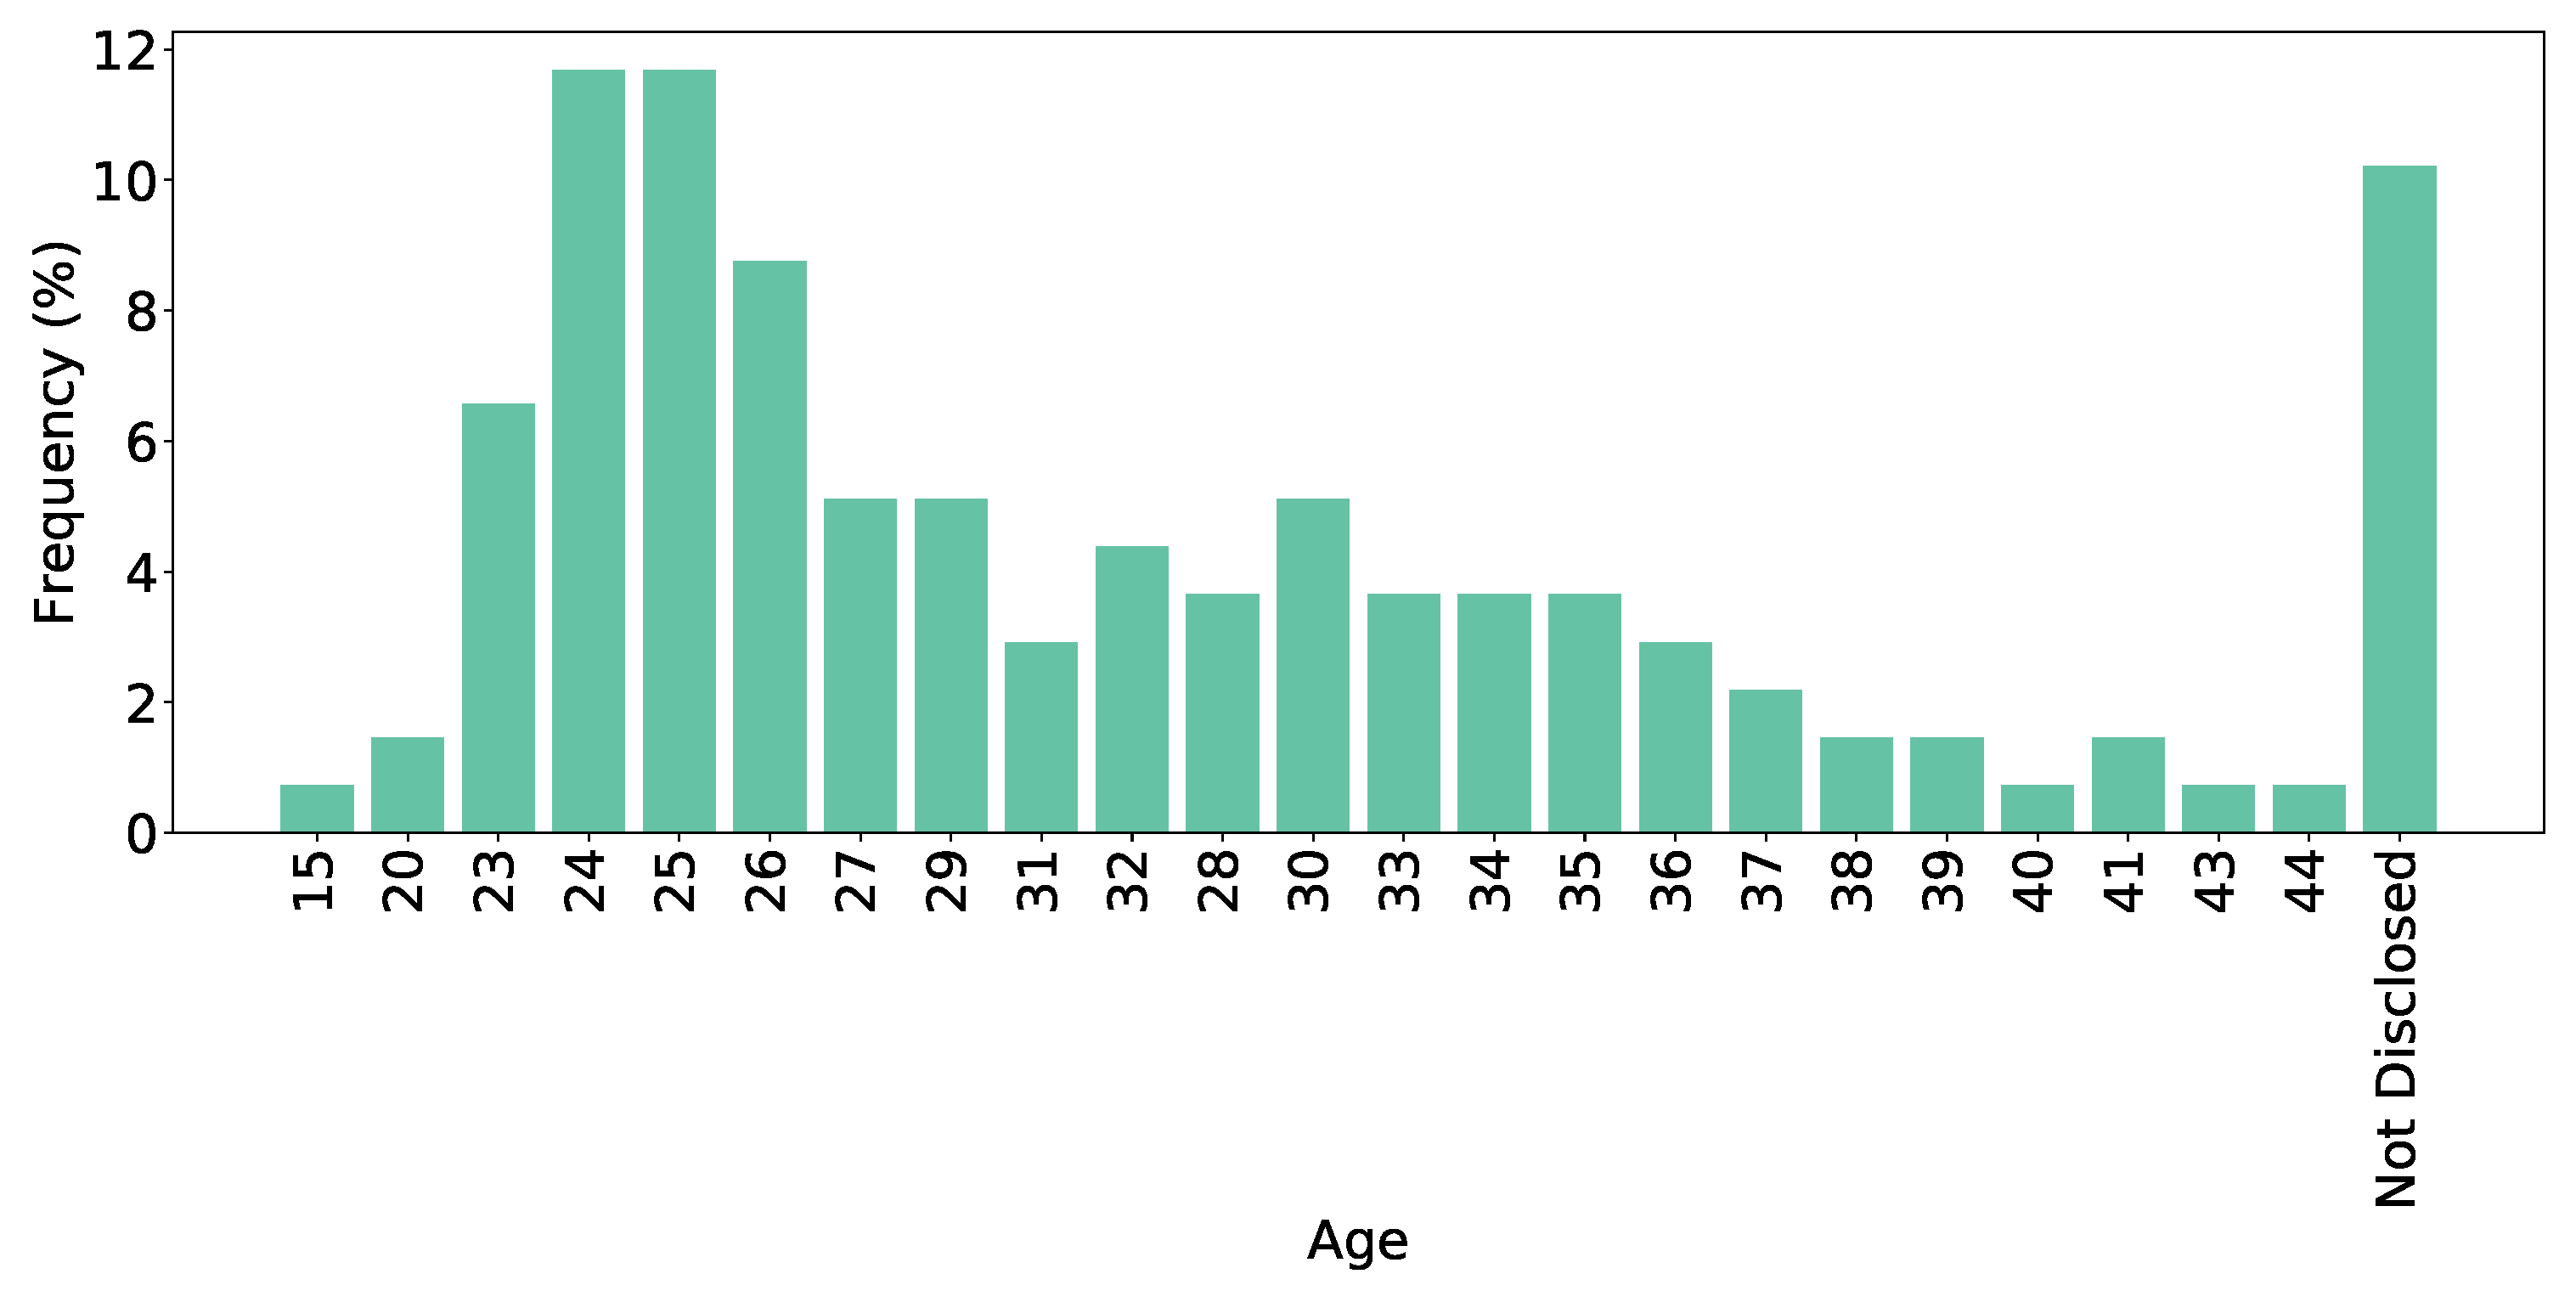
\includegraphics[width=0.8\textwidth]{Figures/Respondents_Age}
  \caption{Respondent's Age}
  \label{fig:age}
\end{figure}

\subsection{Work Experience}
Around 34\% of our respondent's has less than 2 years software development experiences. As the \cref{fig:experience} shows, we have respondent's with various years of work experience which will have positive impact by accumulating valuable results from wider audience base.
\begin{figure}[H]
\centering
  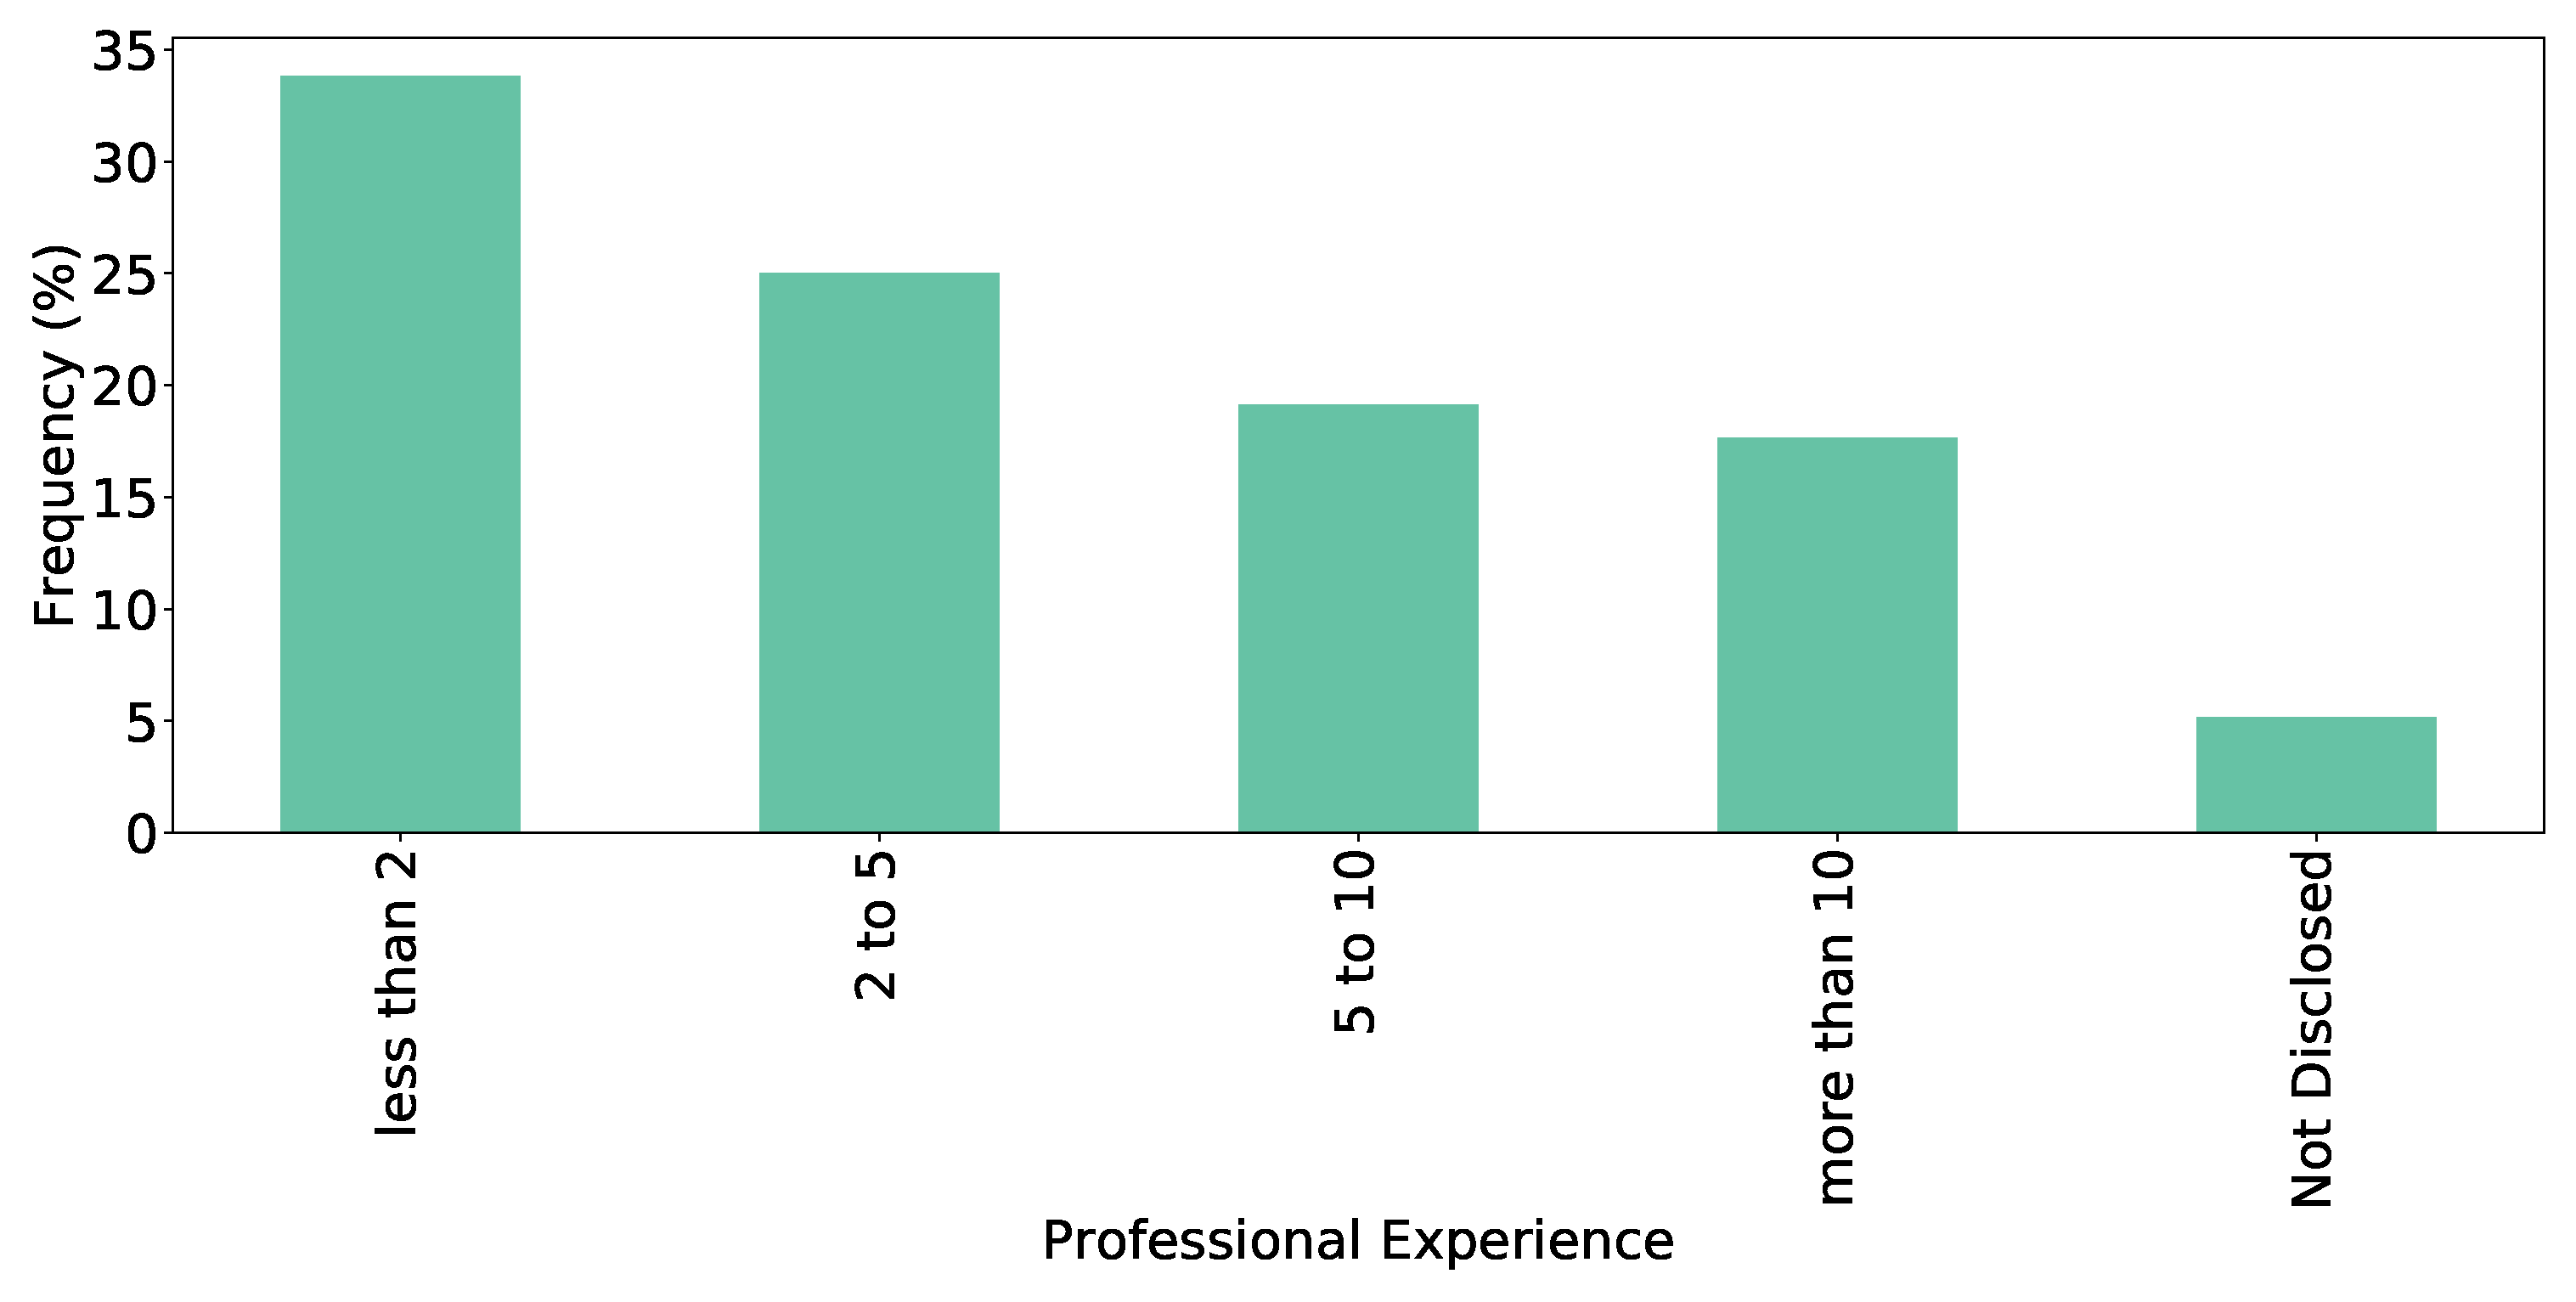
\includegraphics[width=0.8\textwidth]{Figures/Respondents_Experience}
  \caption{Work Experience}
  \label{fig:experience}
\end{figure}

\subsection{Respondent's Current Role}
From the \cref{fig:role} we see most of the respondents were software developers and approximately 15\% of our respondent's are working at manager level post which have appreciable impact on getting expectations from managers.
\begin{figure}[H]
\centering
  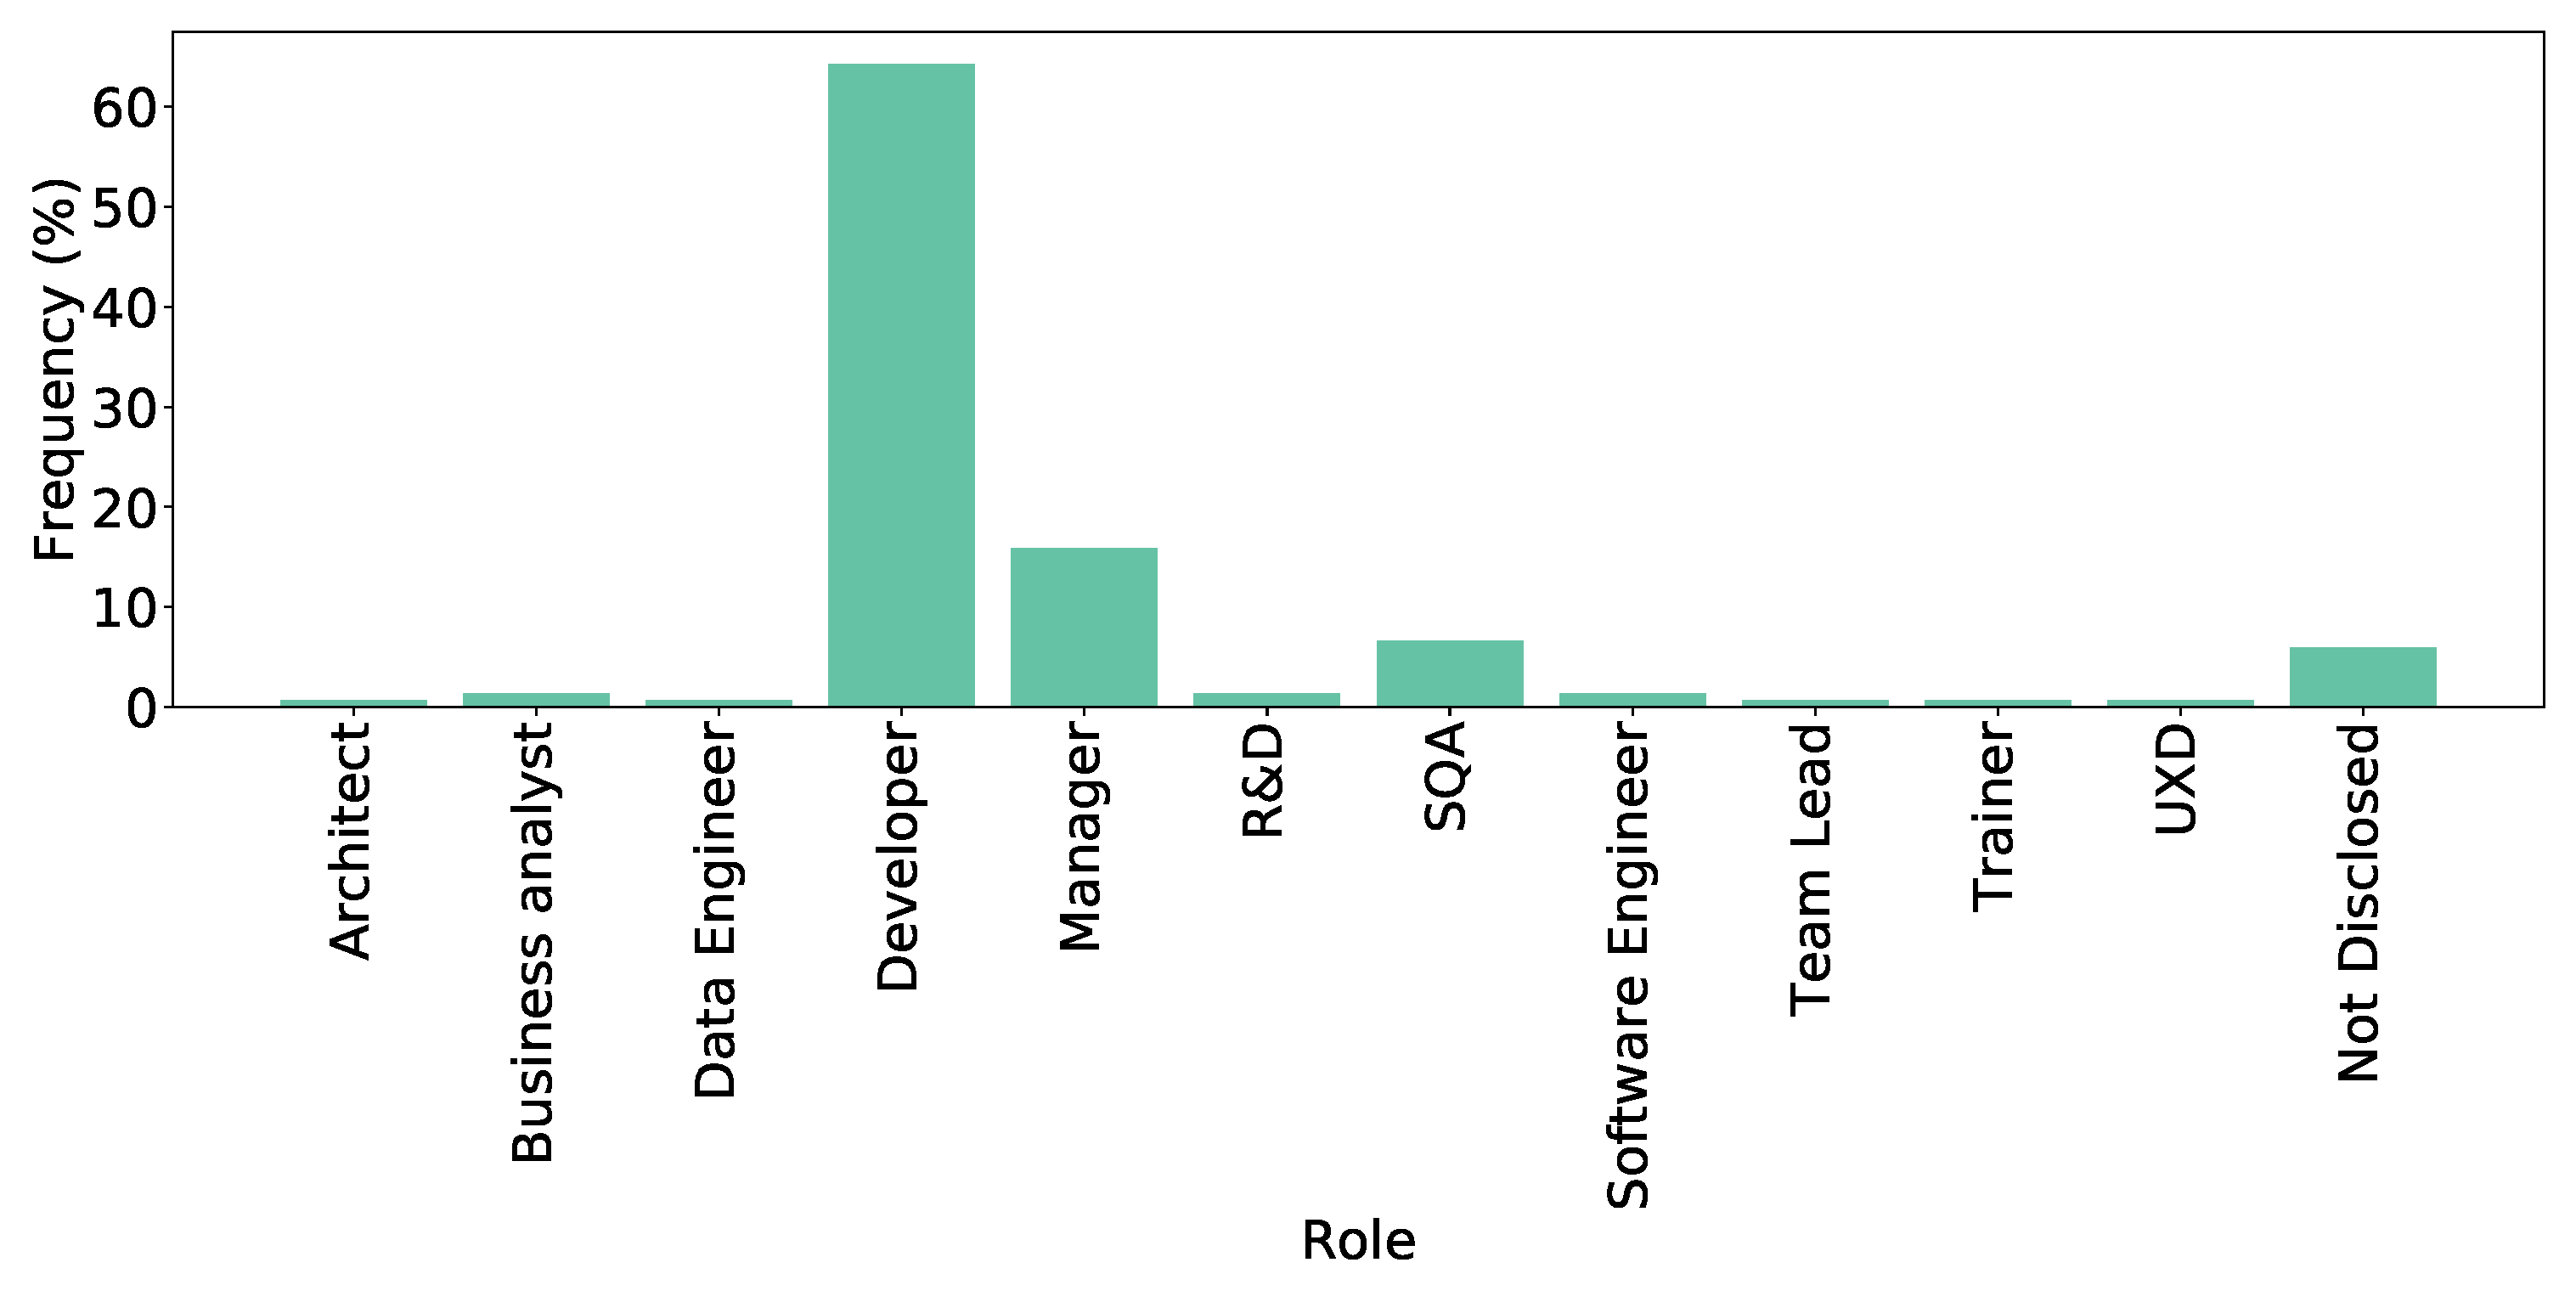
\includegraphics[width=0.8\textwidth]{Figures/Respondents_Role}
  \caption{Respondent's Current Role}
  \label{fig:role}
\end{figure}
\section{Results}

\subsection{RQ1: What software methodology are used in your project?}
\label{RQ1}
Software development methodology in software engineering is a framework that is used to pursue the development of information systems in a very deliberate, structured and methodical way. To find out the overall answer of this question, we report the following results:
\begin{itemize}
\item Software development methodologies (Q 6).
\item Requirements gathering (Q 7).
\item Most time consuming software development activities (Q 8).
\end{itemize}

\subsubsection{Software development methodologies}
The most-widely used model is Agile with usage rate of 64\%. The next widely-used model is scrum with usage rates of 46\%. The other methodologies has lower usage rates, namely: pair programming (20\%), Waterfall (12\%) etc. From the study we see that the most acceptable model that was regularly and always used is the agile model in Bangladesh but the usage of the scrum (44\%) in New Zealand has greater usage followed by agile (30\%) \citep{Wang2018} and in Turkey, waterfall is mostly used based on the earlier 2015 survey \citep{Garousi2015}. Again, in both Bangladesh and New Zeland, extreme programming (XP) has a lower percentage of usage.
\begin{figure}[htbp]
\centering
  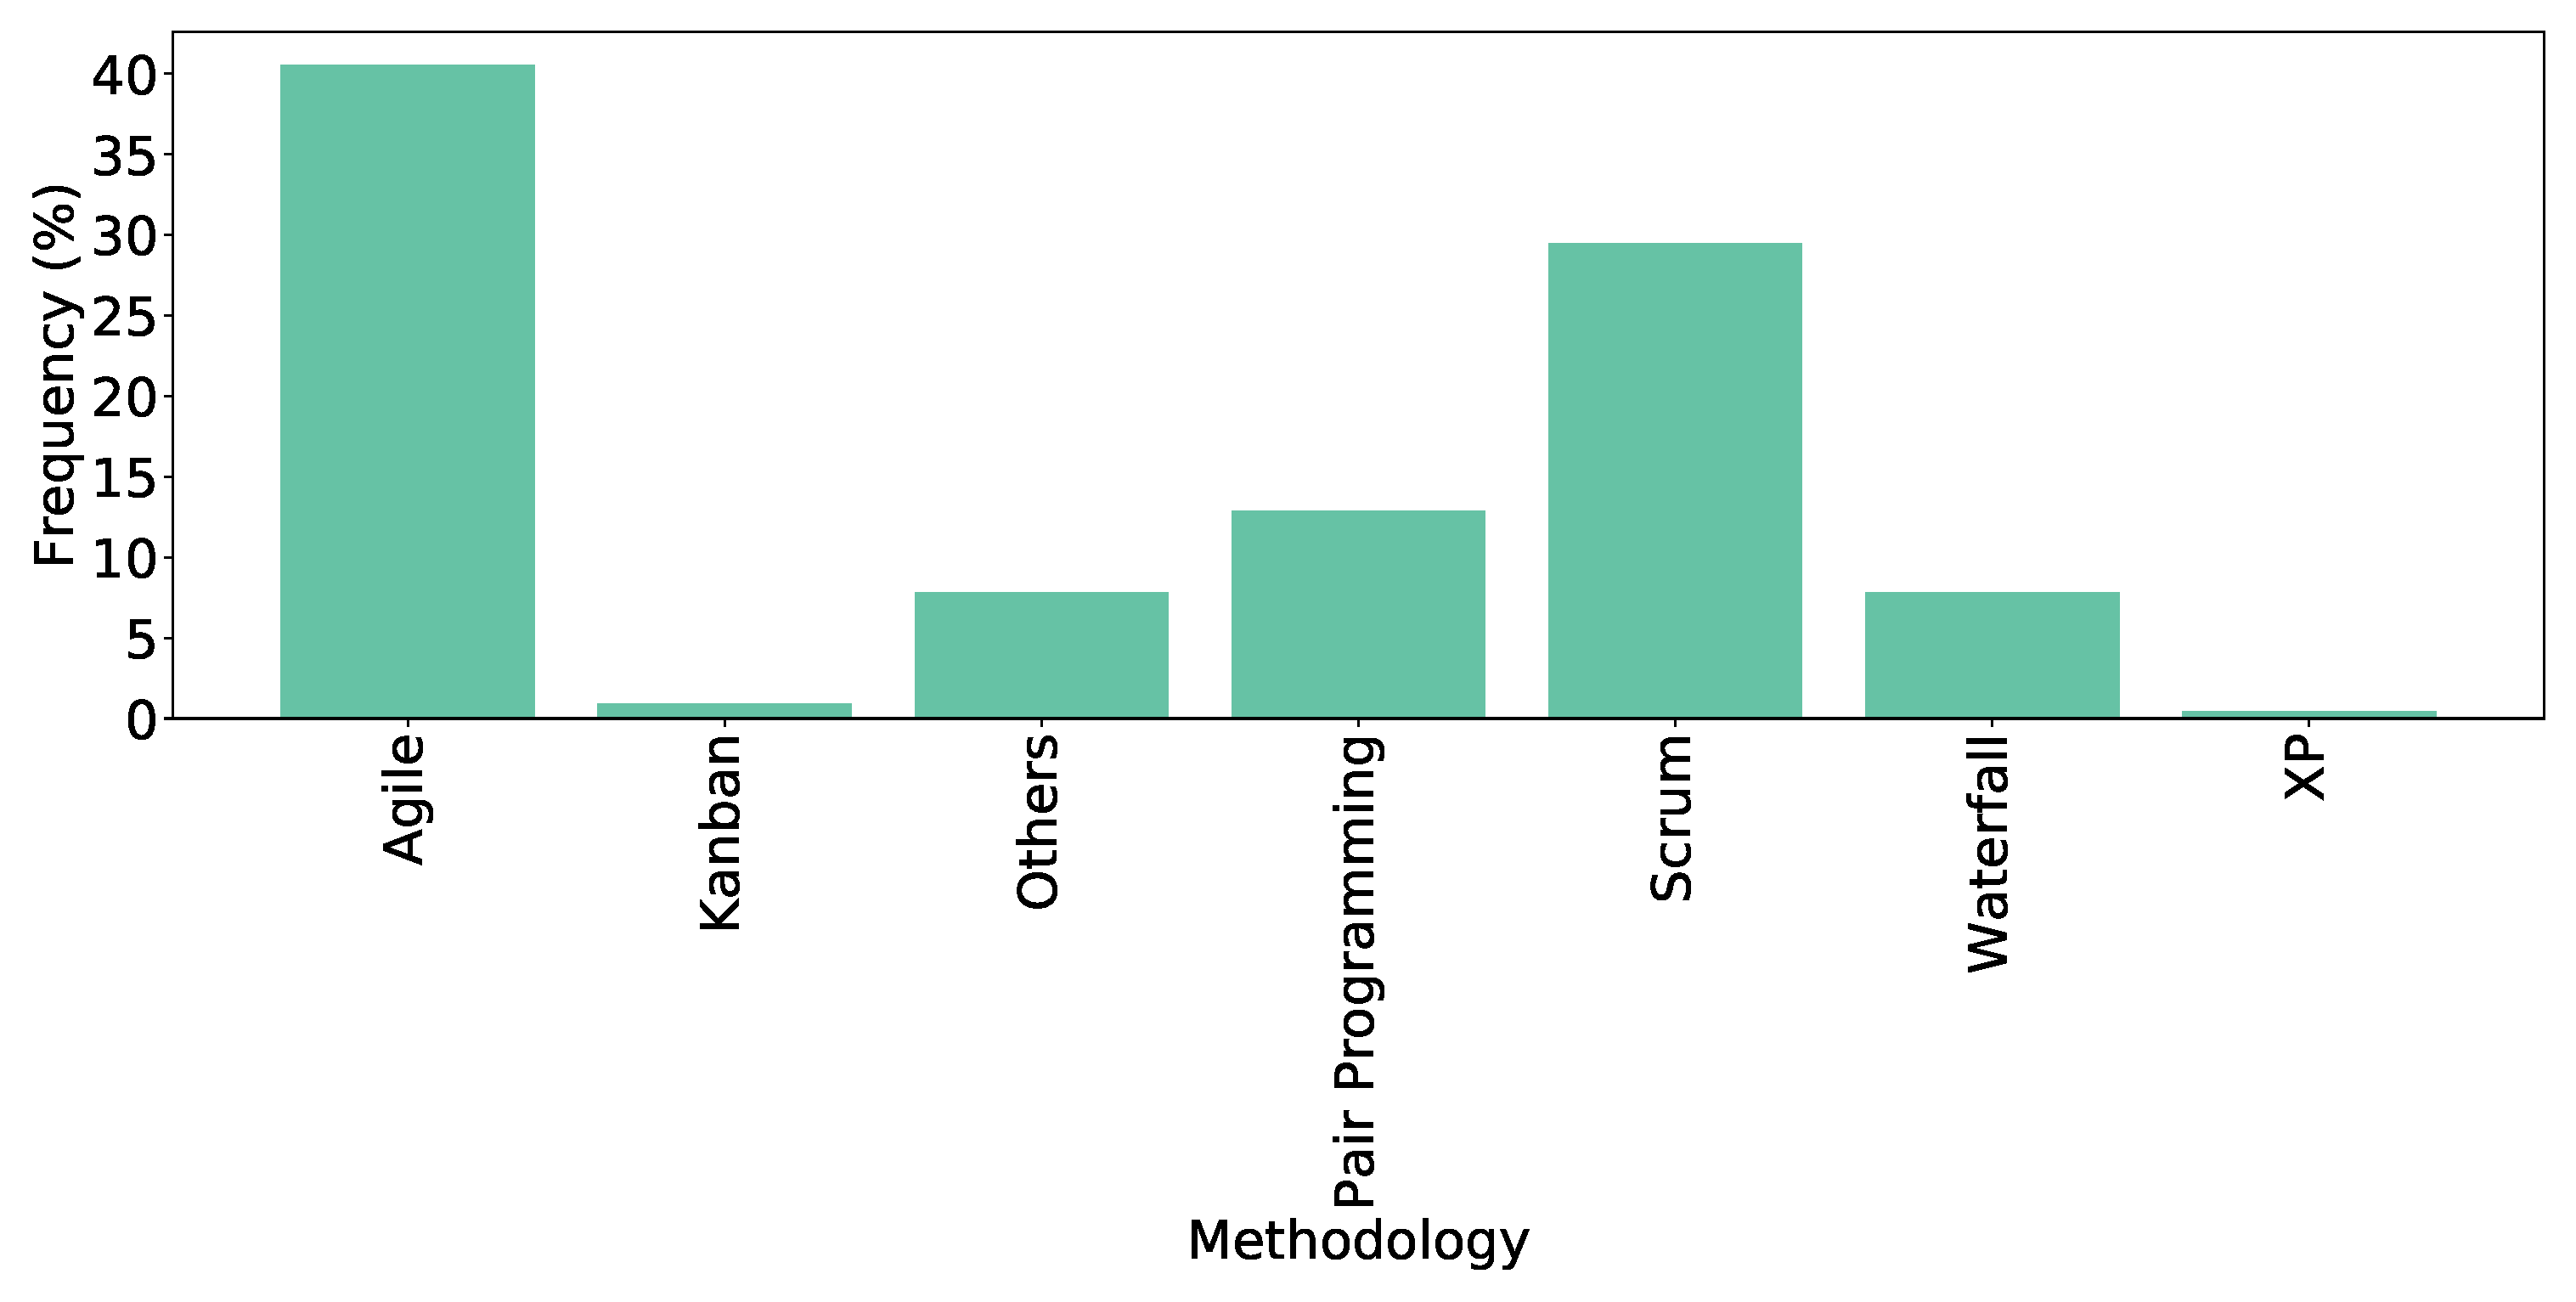
\includegraphics[width=0.8\textwidth]{Figures/Respondents_Methodology}
  \caption{Software development methodologies}
  \label{fig:methodologies}
\end{figure}

\subsubsection{Requirements Gathering}
The most critical activity that always arises during software development is the collecting requirement of the proposed system. According to \cref{fig:requirements}, using plain text (44\%) and story board (41\%) are the most widely used requirements gathering. This result is similar with the survey of Vonken et al. \citep{Vonken2012}. From their study we can find that the textual description of specifying requirements is a firm favourite in Netherlands. The other requirements gathering usage rates are: Use case (36\%), GUI prototype (35\%), grooming session (30\%) etc. This is an important finding that requires further analysis for causes and to analyze the potential effects of not documenting requirements.
\begin{figure}[htbp]
\centering
  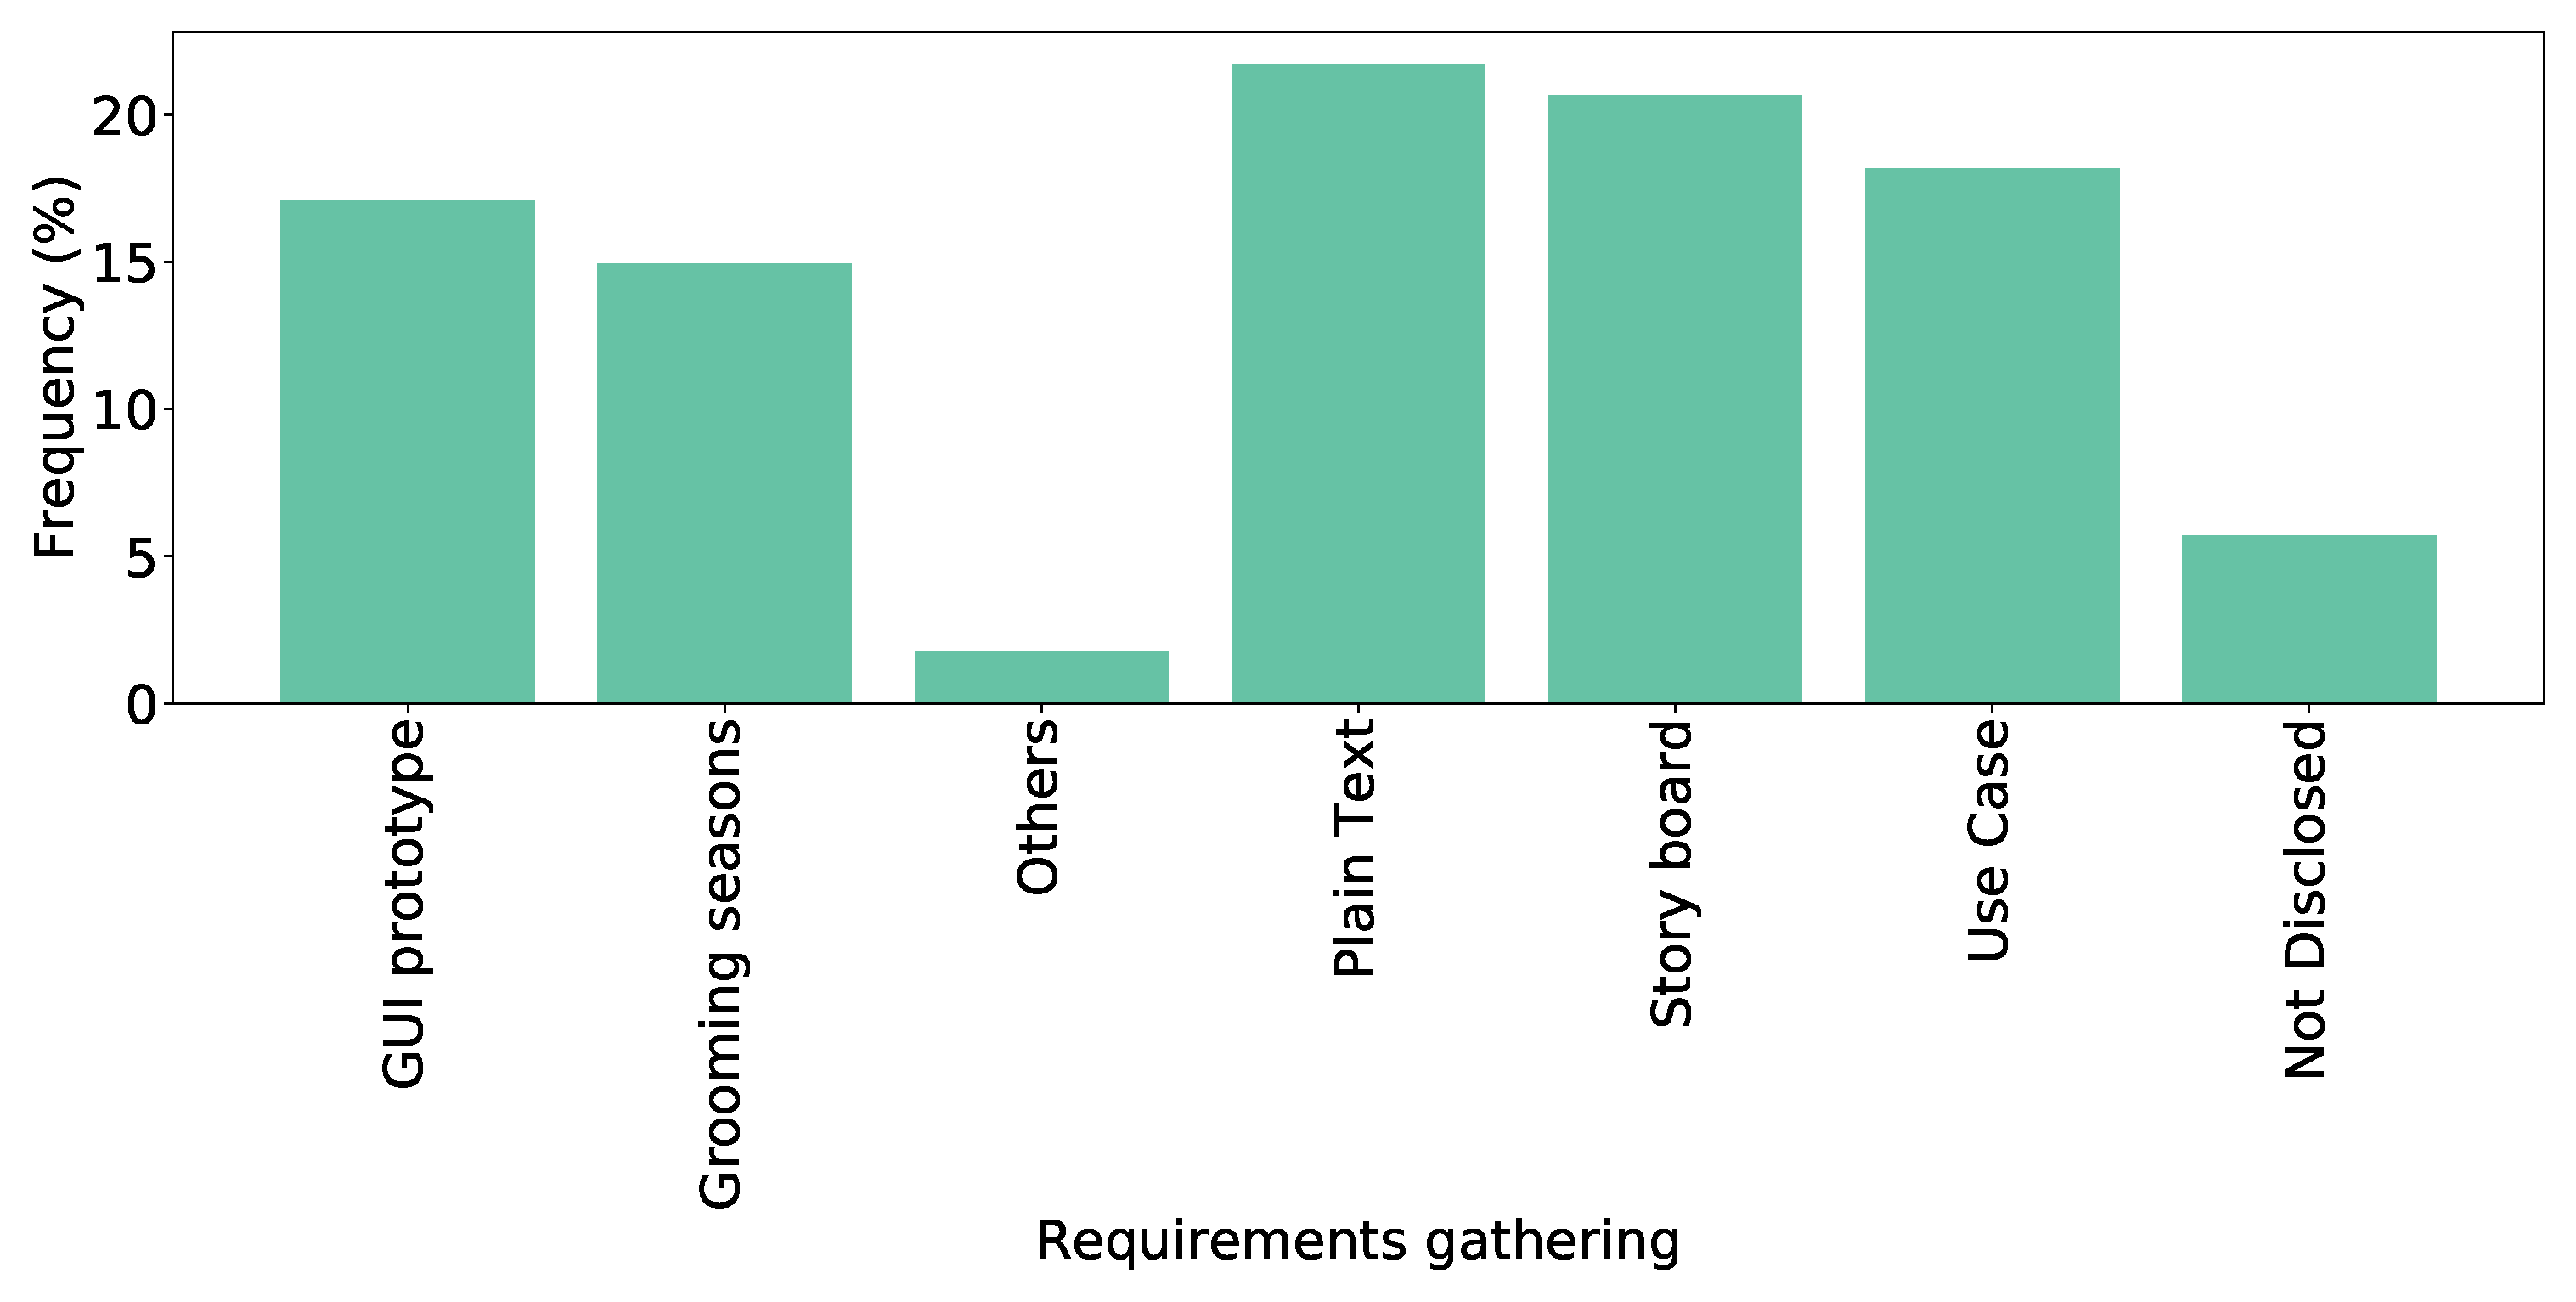
\includegraphics[width=0.8\textwidth]{Figures/Requirements_Gathering}
  \caption{Requirements gathering}
  \label{fig:requirements}
\end{figure}

\subsubsection{Development activities timeline}
In this section participants were asked about the most time consuming software developing activities they had spend. As we see in \cref{fig:activities}, most of the time spent in implementation stage according to 65\% our respondents and requirement analysis stage requires second most according to 45\% response. The other usages are: Program design (37\%), project planning (30\%), testing (19\%), maintenance (17\%) etc. According to study \citep{Wang2018}, most time was spent on implementation and coding and relatively less time was spent on maintenance in Bangladesh and New Zealand. But requirement analysis, the activity, requires the second most time to spend in Bangladesh where in New Zealand, it is testing (36\%) practices.

\begin{figure}[htbp]
\centering
  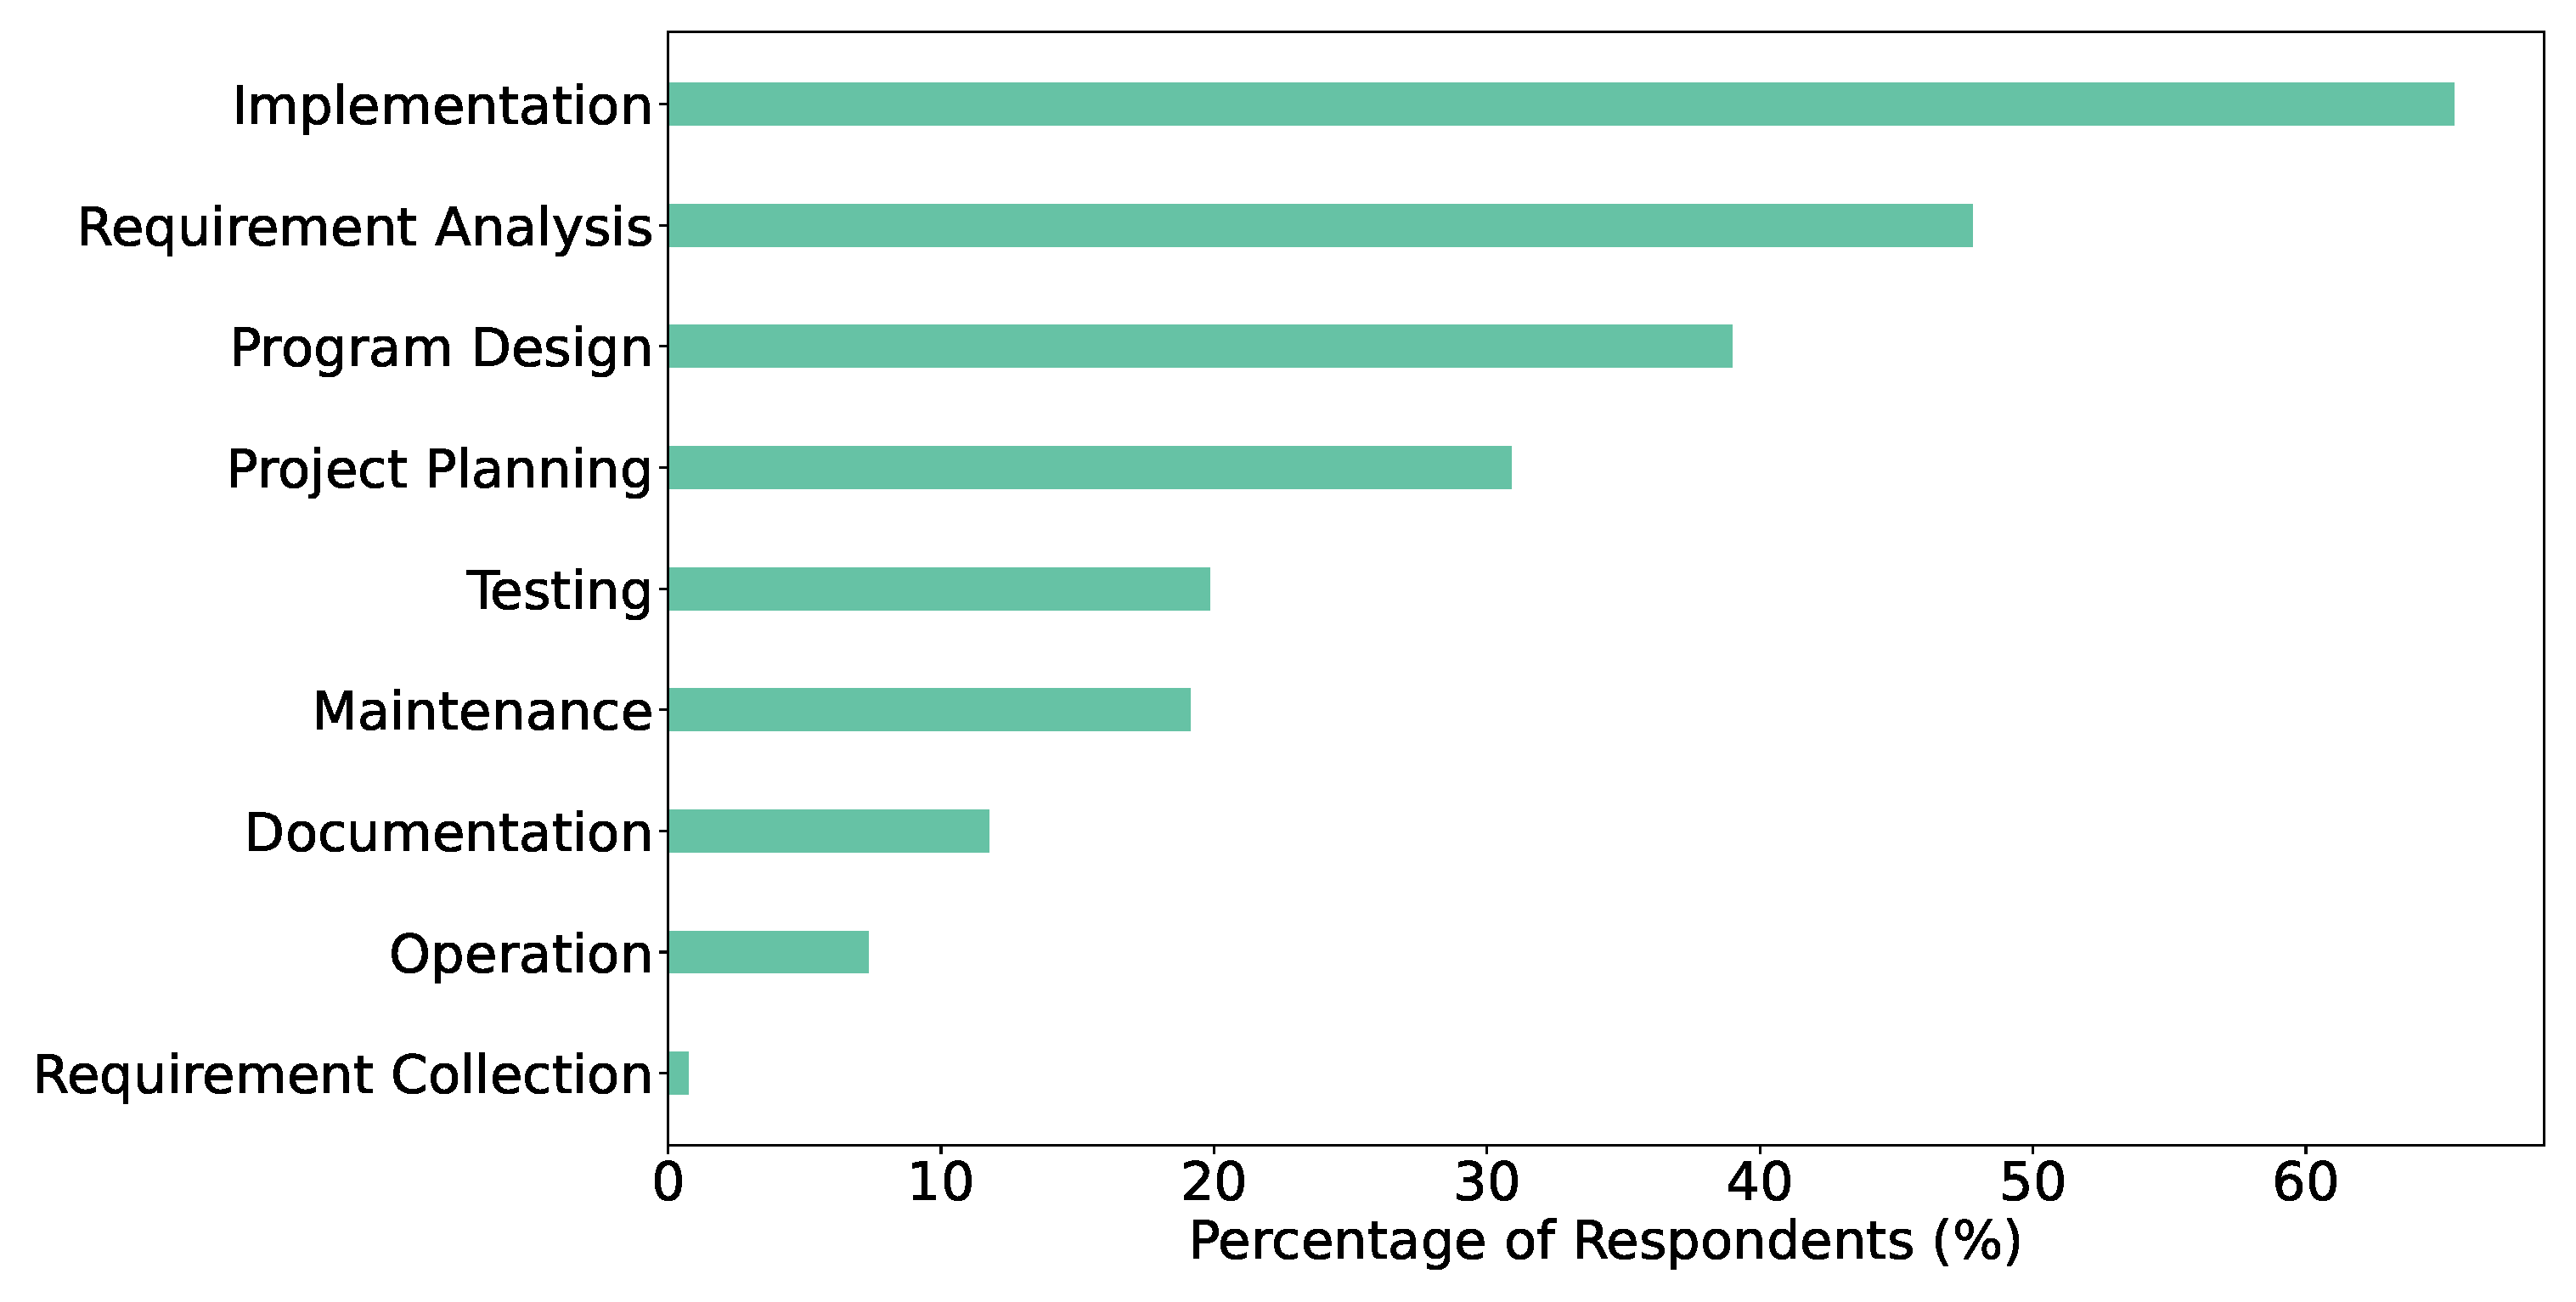
\includegraphics[width=0.8\textwidth]{Figures/Respondents_Activities}
  \caption{Software development activities}
  \label{fig:activities}
\end{figure}
\subsection{RQ2: Which implementation technologies and tools are adopted by software development professionals?}
\label{RQ2}
Our survey included five questions to find technologies and tools that are adopted by software development professionals. To answer this question fully, we report the following results:
\begin{itemize}
\item Technology Platform (Q 9).
\item Operating System (Q 10).
\item Programming Language (Q 11).
\item Framework (Q 12).
\item IDE (Q 13).
\end{itemize}

\subsubsection{Technology Platforms}
Participants were allowed to choose multiple options. As shown in \cref{fig:platforms}, most of the respondents (80\%) worked in web platform. The rests were mobile (45\%), Desktop (30\%), Embedded/IOT (8\%). Most respondents develop products and services for web platforms in both Bangladesh and New Zealand based on \#.
\begin{figure}[htbp]
\centering
  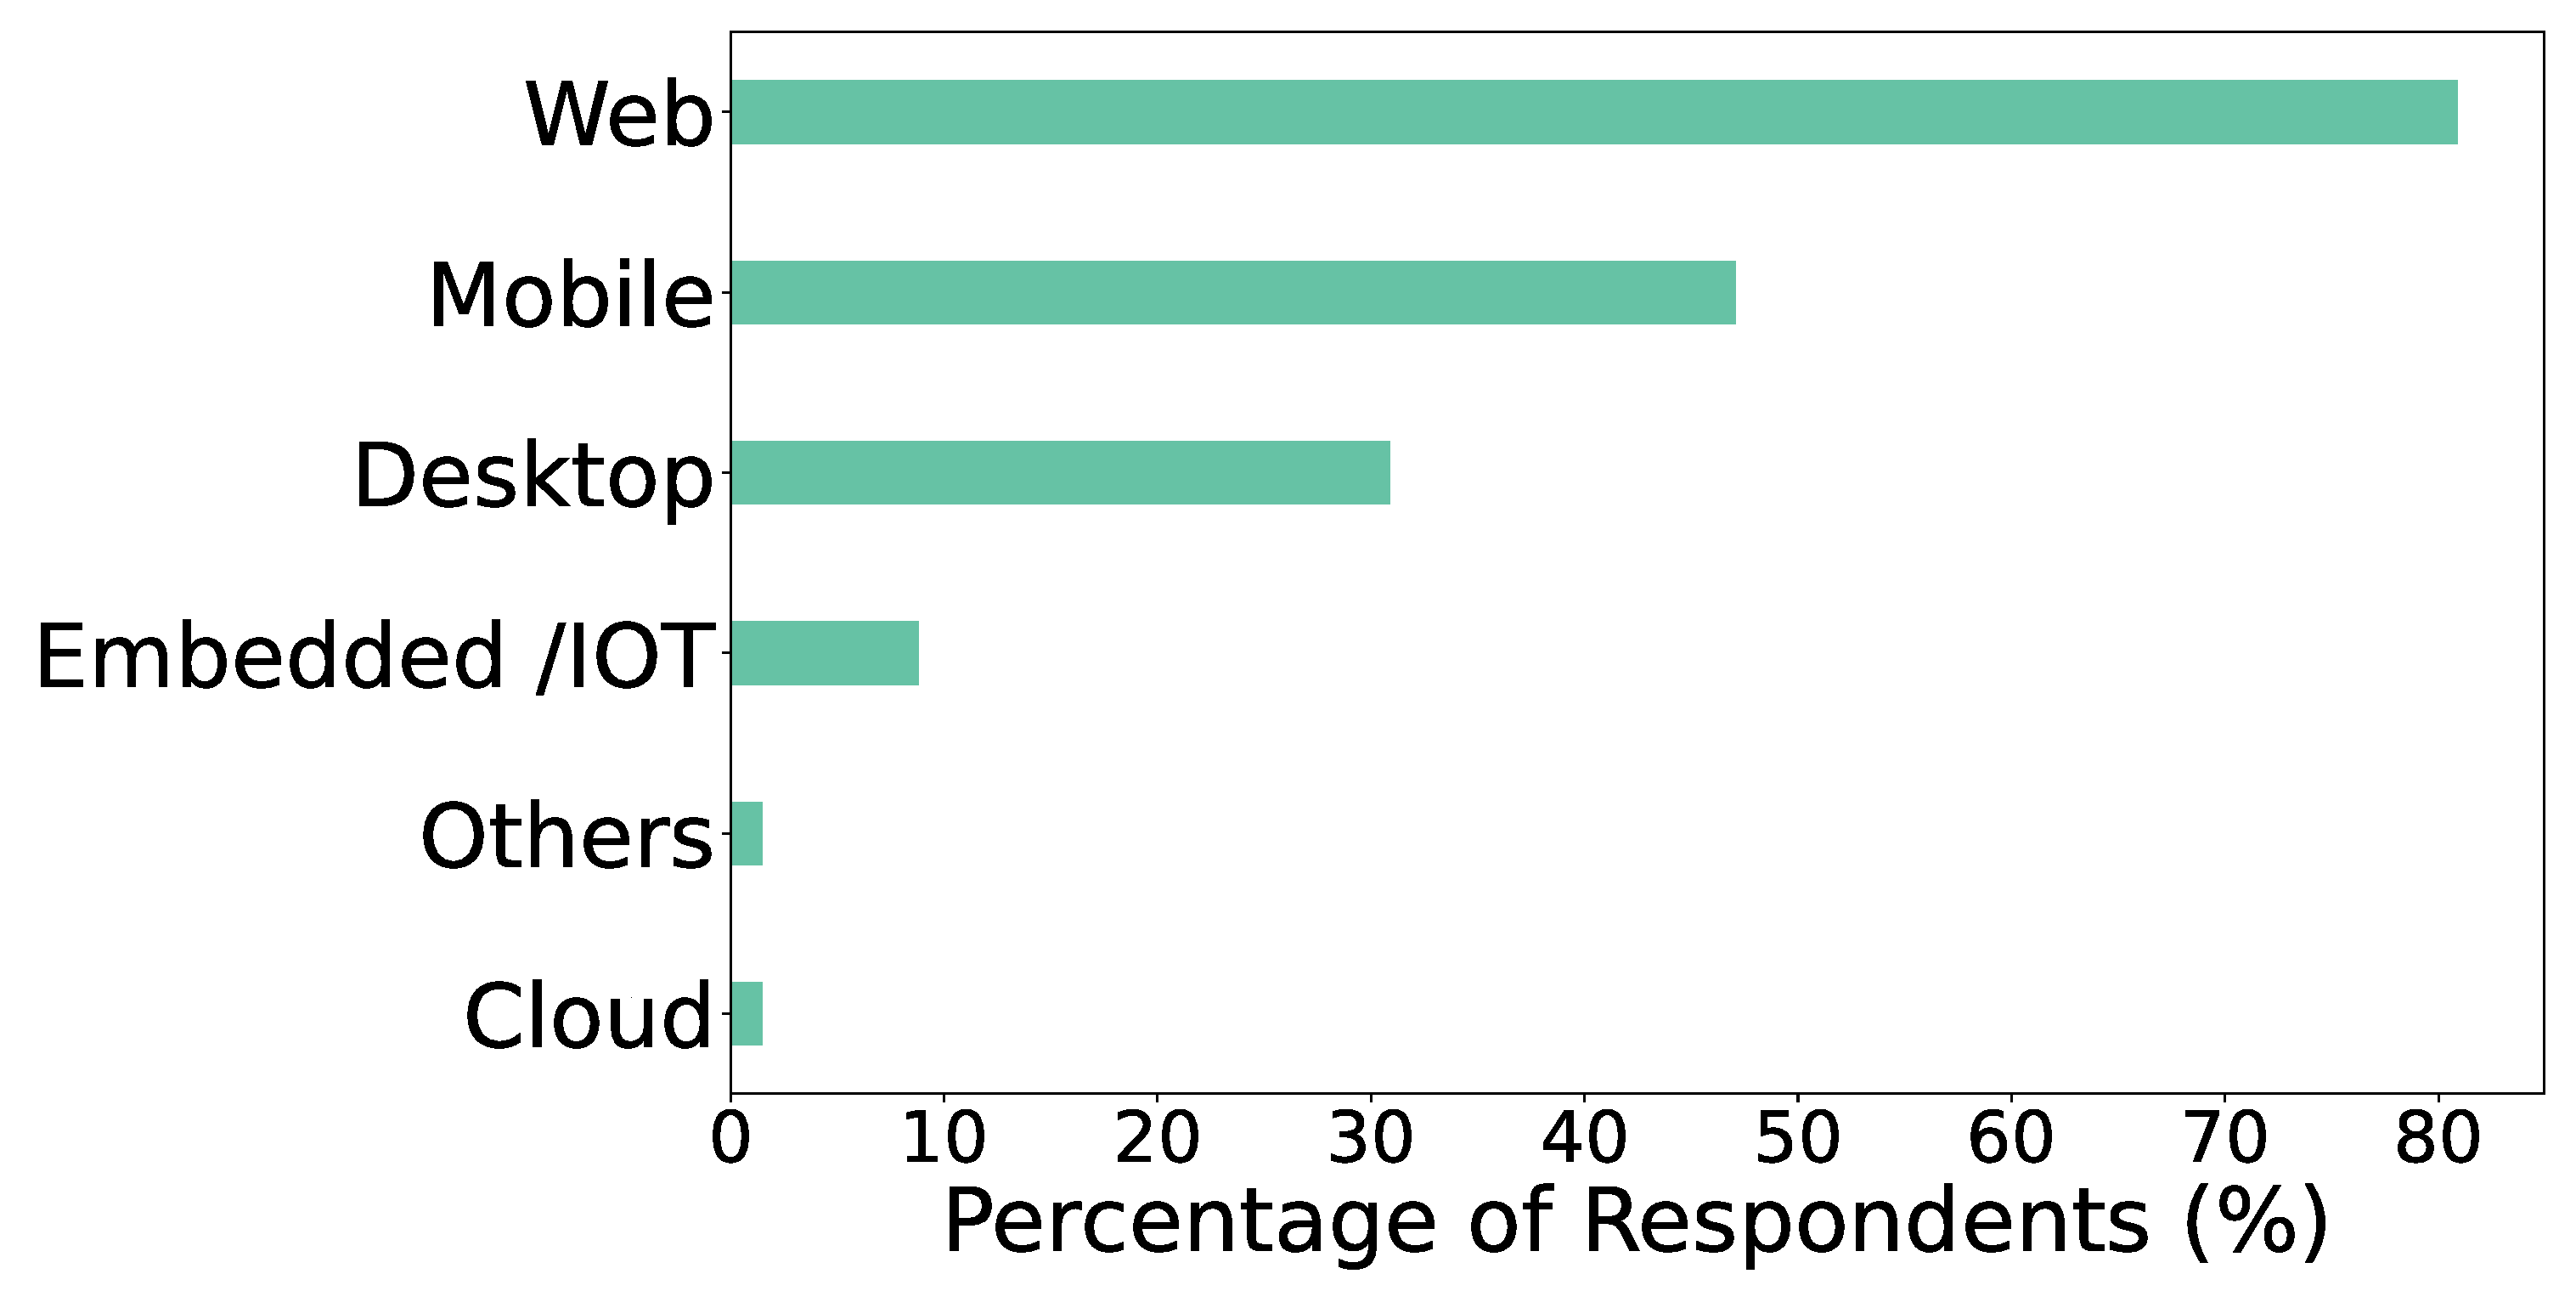
\includegraphics[width=0.8\textwidth]{Figures/Respondents_Technologies}
  \caption{Technology Platforms}
  \label{fig:platforms}
\end{figure}

\subsubsection{Operating Systems}
Most of our respondent's used linux based operating system (56\%). The second best used operating system is windows (45\%). Windows is mostly used among developers of New Zealand based on
the Survey \#, but linux is mostly used in the case for Bangladeshi developers.

\begin{figure}[htbp]
\centering
  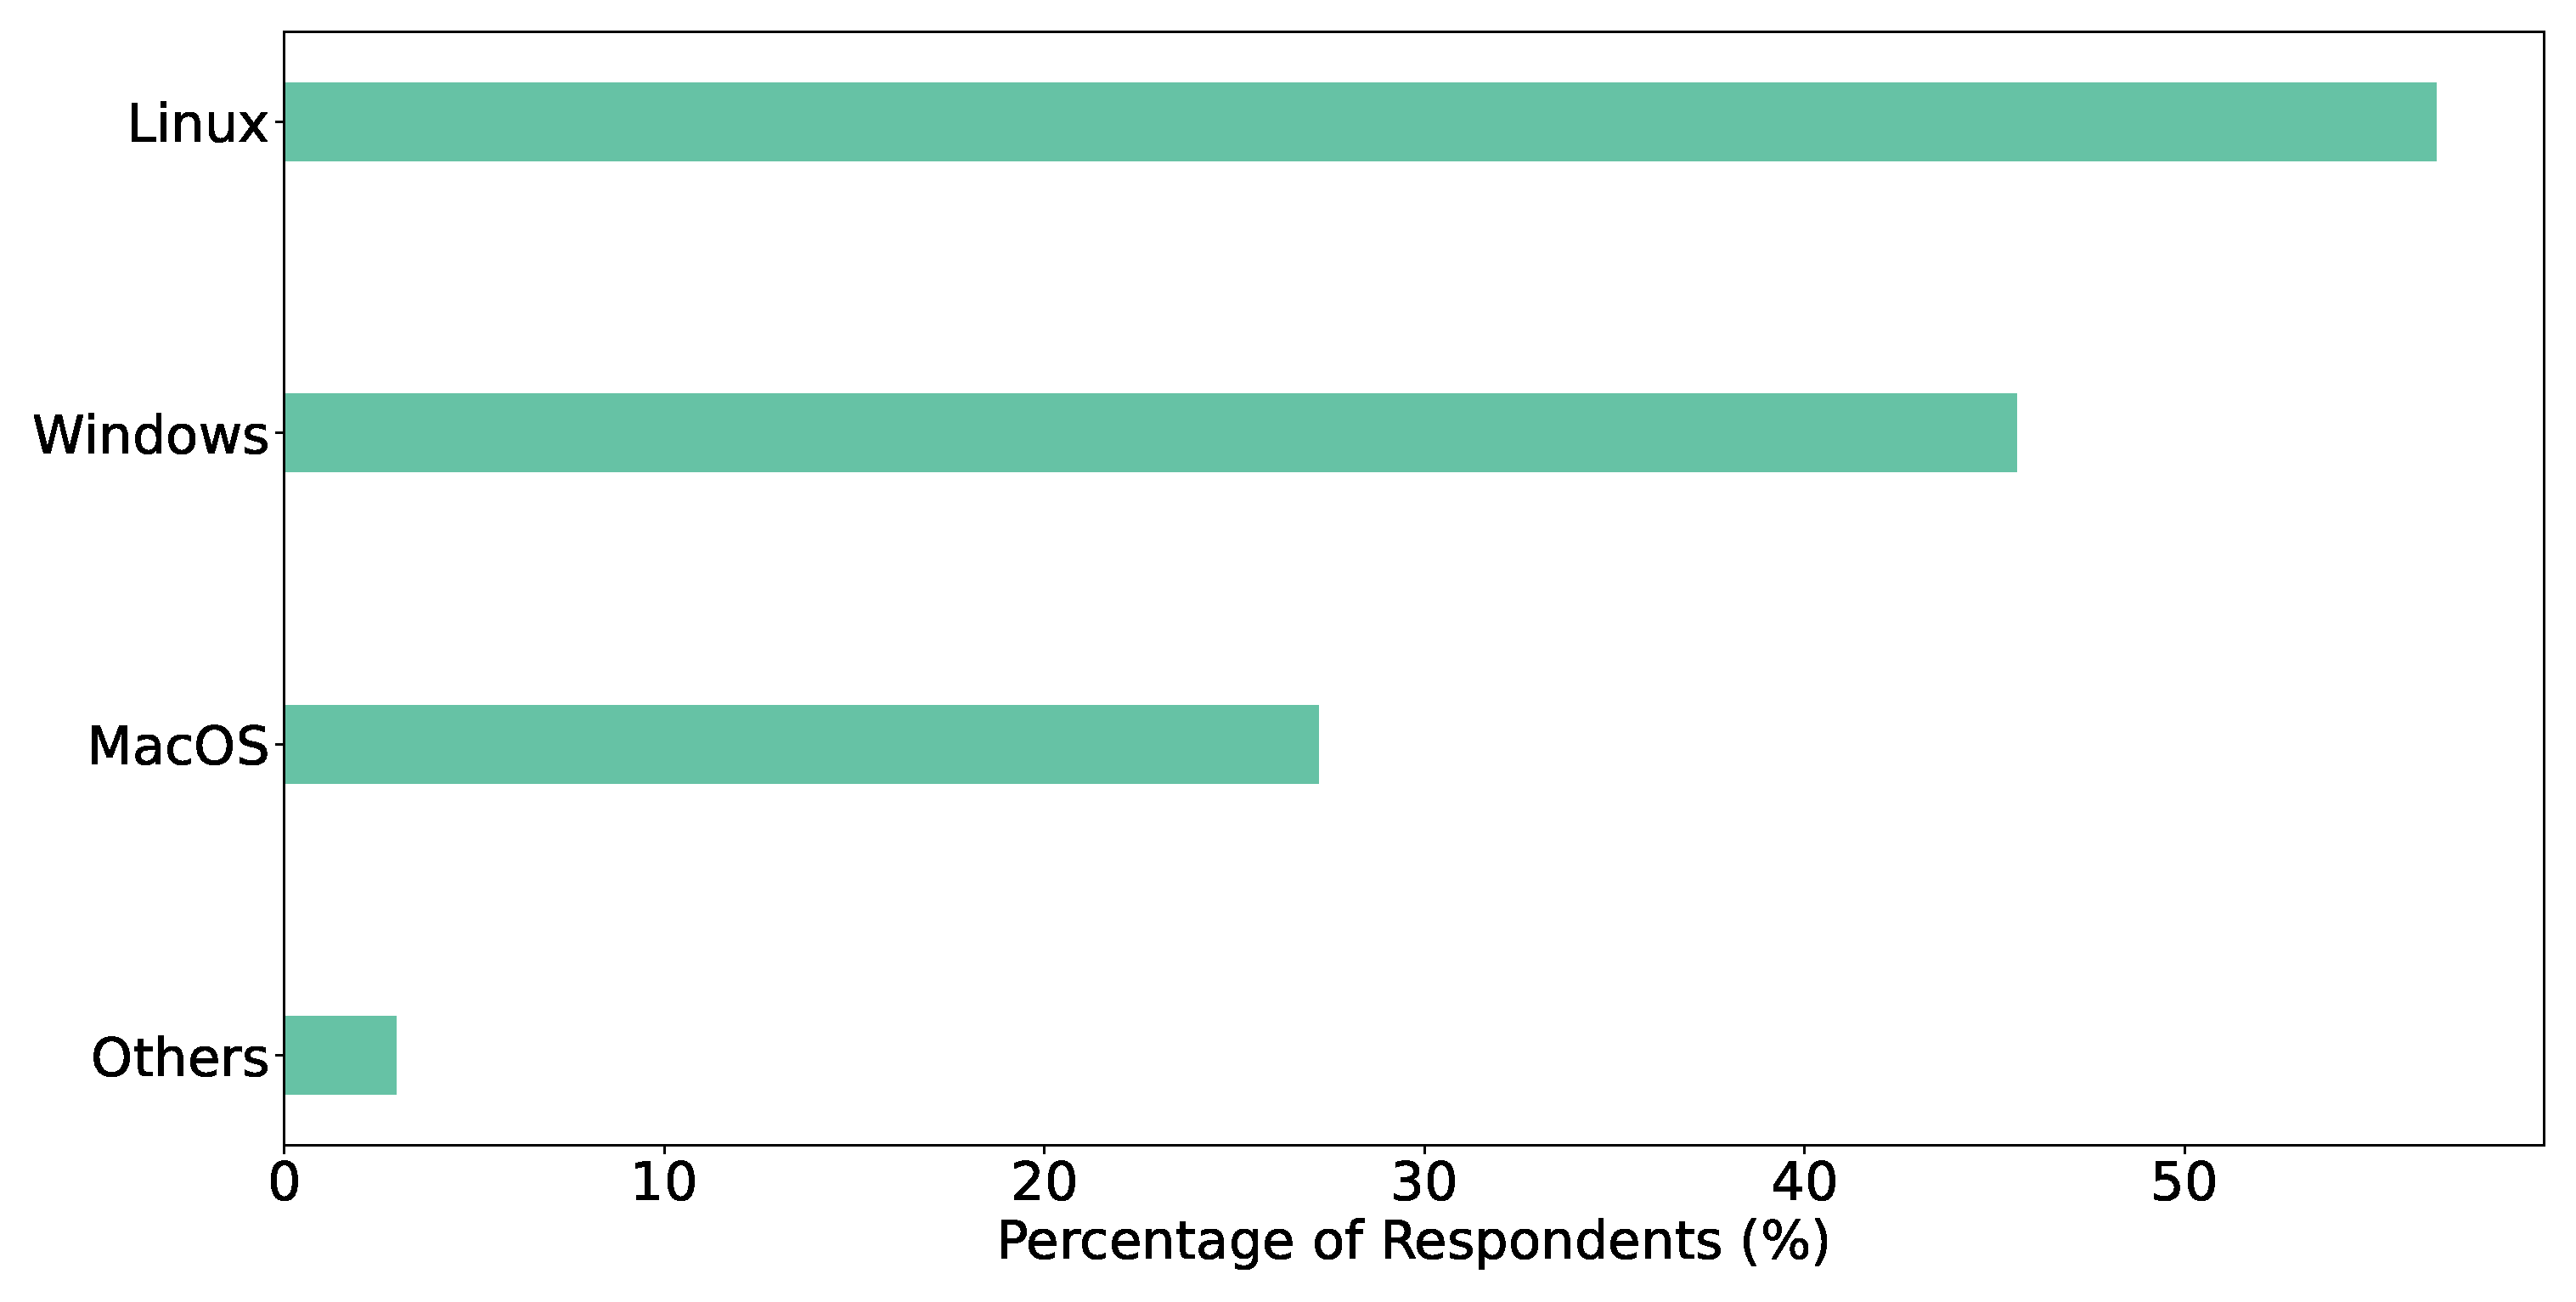
\includegraphics[width=0.8\textwidth]{Figures/Respondents_os}
  \caption{Operating Systems}
  \label{fig:os}
\end{figure}

\subsubsection{Programming Languages}
According to \cref{fig:languages}, around 61\% of our respondent's used Java and Javascript each. Other languages like php (25\%), python (25\%), c\# (18\%) are also used which indicates that the software engineers are not inclined towards a single specific language. Also the choice of programming languages used for development can have important inferences for the testing practices of a software company. Based on \#, Java ranks quite low in New Zealand where it is the second most used in Bangladesh and the mostly used language in Turkey (\#). Again, python did not get a respective place in the rank of used languages in New Zealand but it is used significantly in Bangladesh.

\begin{figure}[htbp]
\centering
  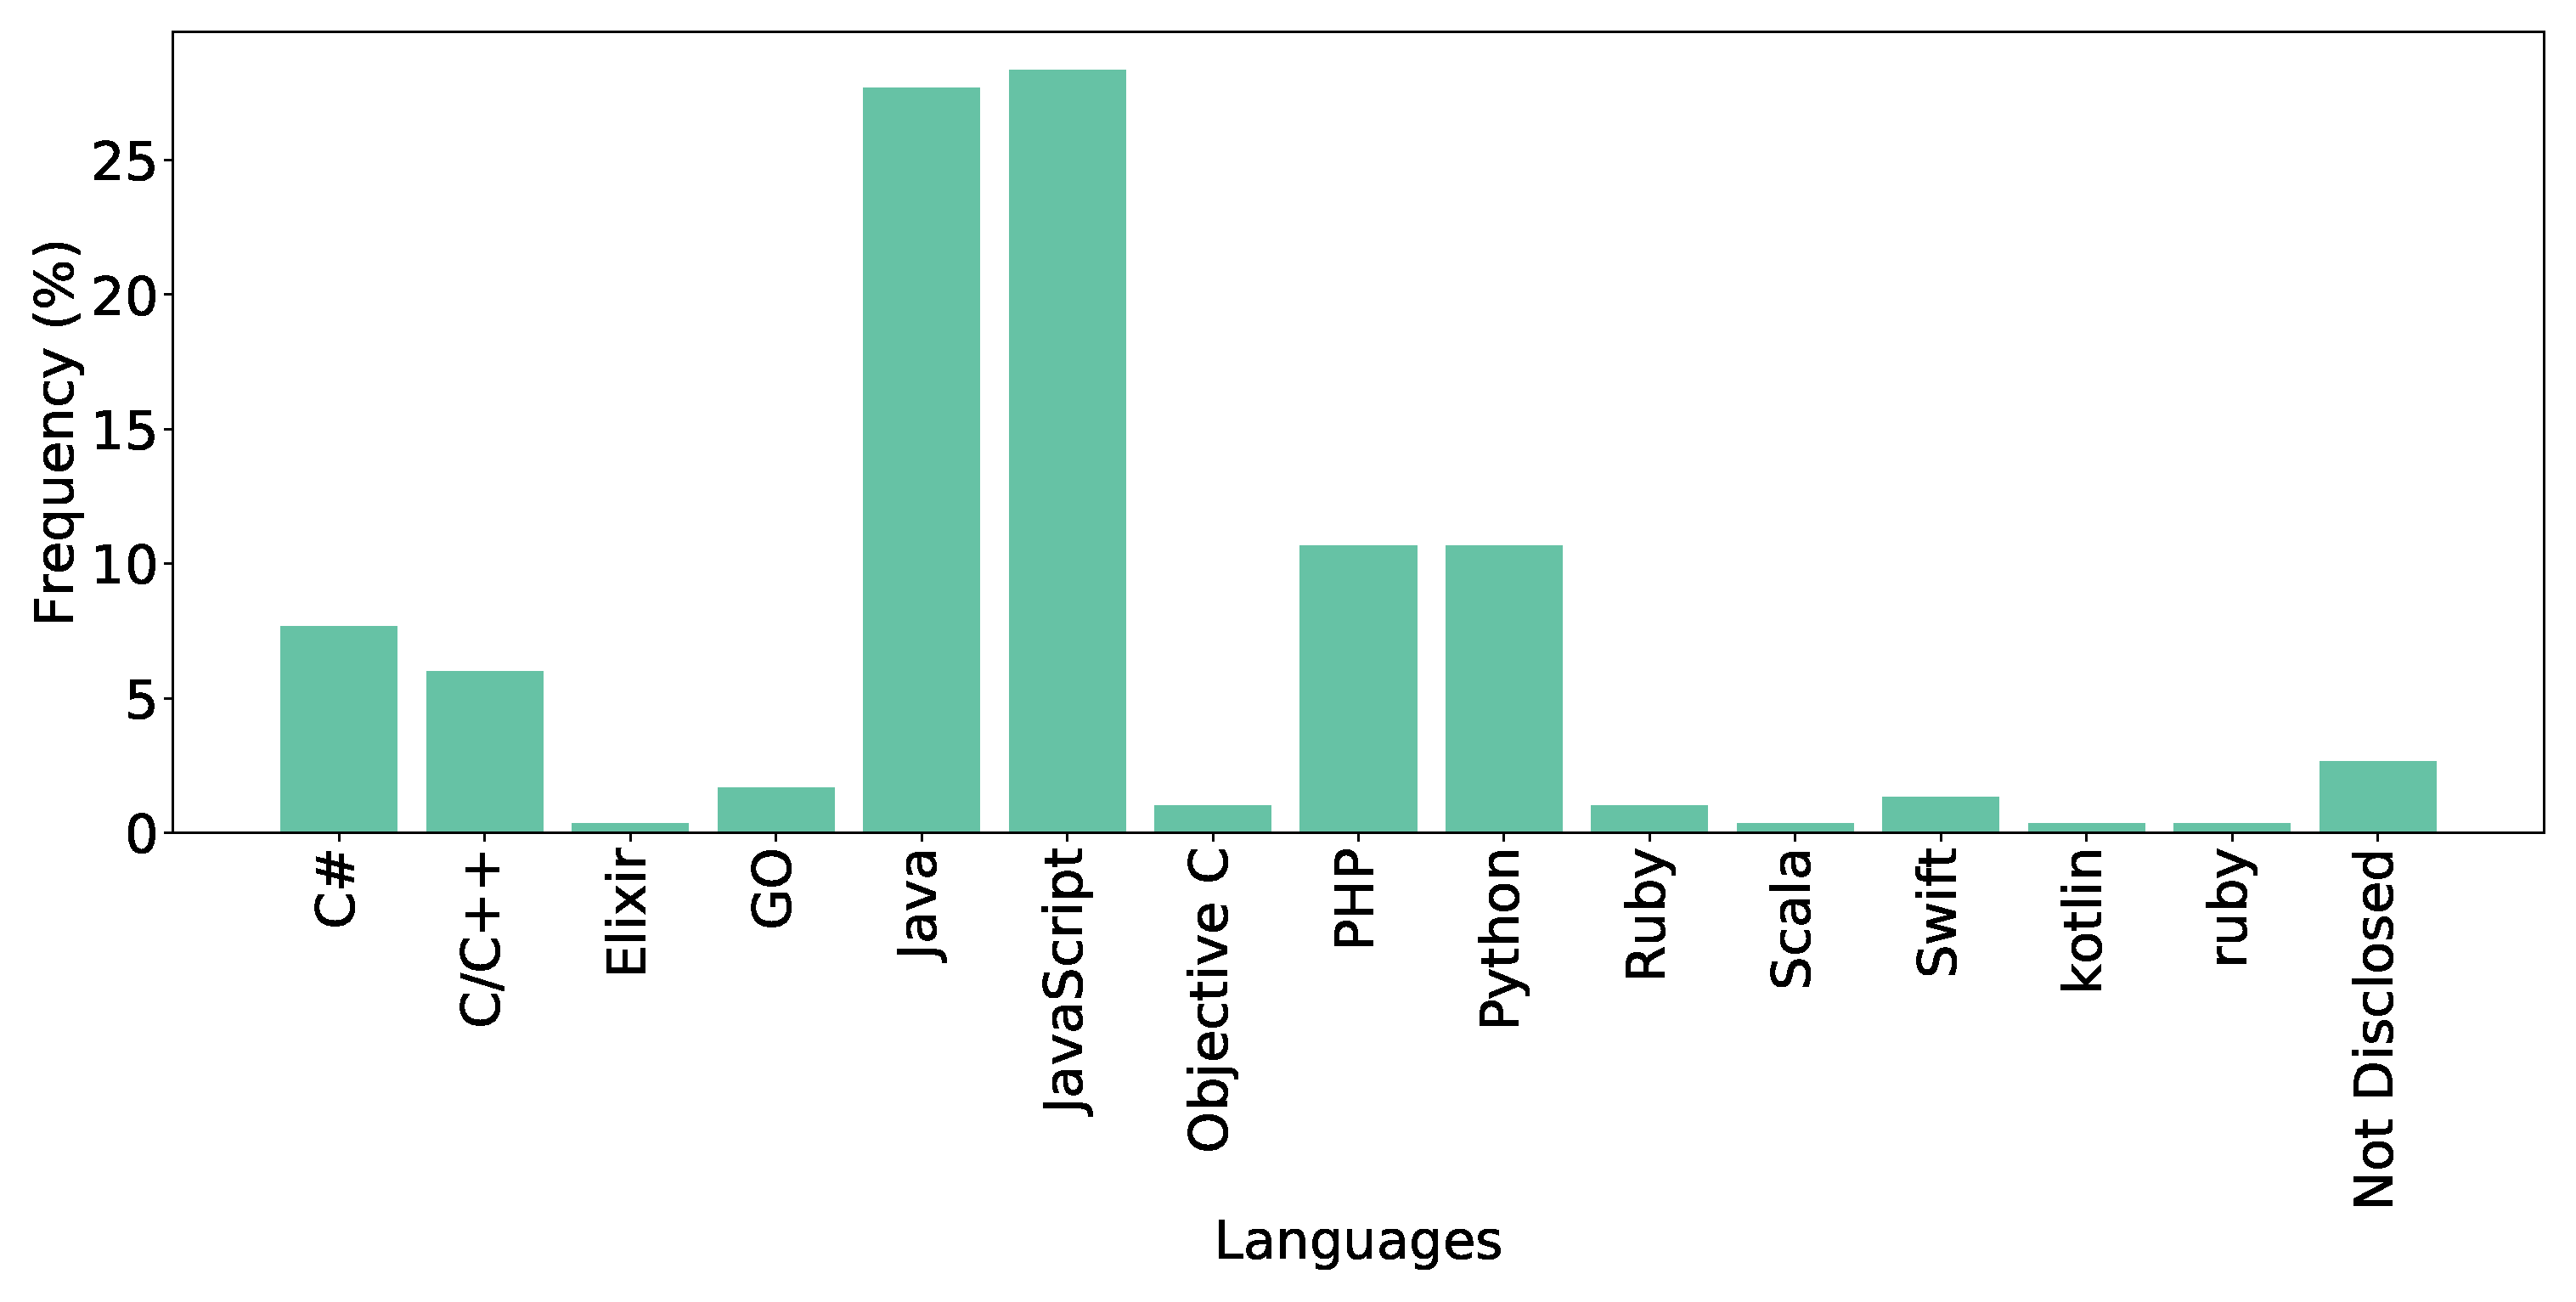
\includegraphics[width=0.8\textwidth]{Figures/Respondents_languages}
  \caption{Languages used in software development}
  \label{fig:languages}
\end{figure}

\subsubsection{Frameworks used in development}
As shown in \cref{fig:frameworks}, variety of frameworks have been used during development. Spring boot (37\%) is the mostly used framework in the industry. ASP.NET, Django and Laravel are used in same proportion (14\%).
\begin{figure}[htbp]
\centering
  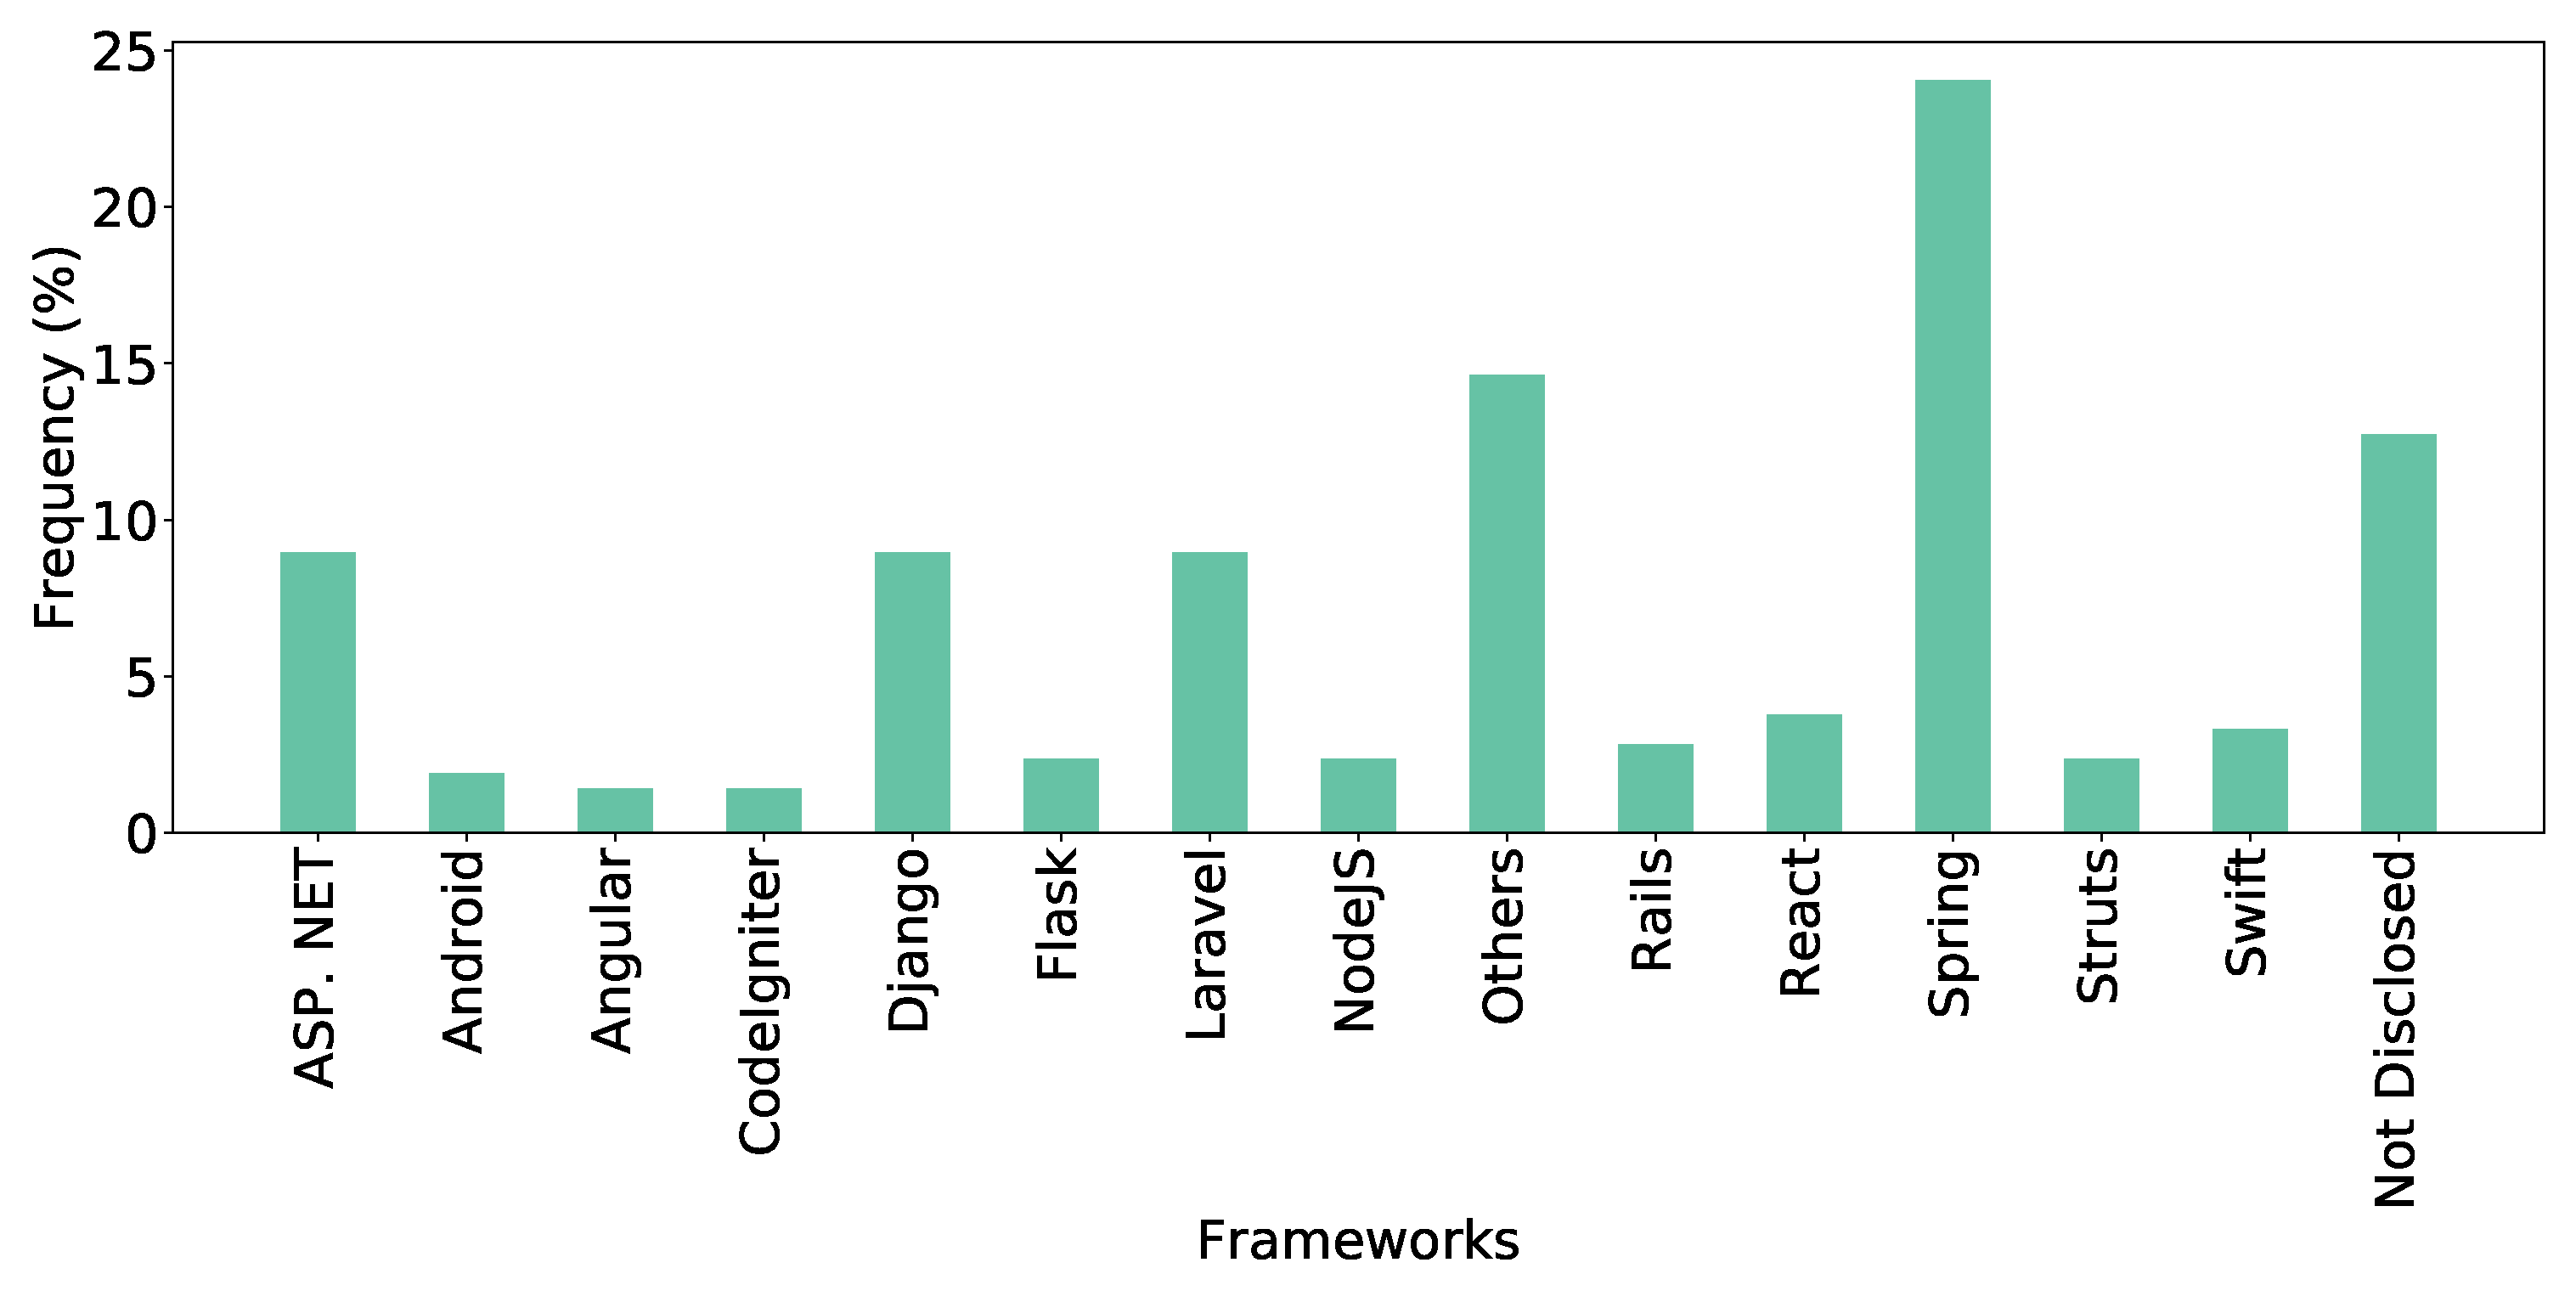
\includegraphics[width=0.8\textwidth]{Figures/Respondents_frameworks}
  \caption{Frameworks}
  \label{fig:frameworks}
\end{figure}

\subsubsection{IDE's used by the respondent's}
According to \cref{fig:IDEs}, IntelliJ, a Java integrated development environment for developing computer software for enterprise, mobile, and web development used by most of the respondents (43\%). The other IDEs used in SE industries are: visual studio (30\%), Eclipse (24\%), PyCharm (16\%), NetBeans (10\%), Android Studio (6\%).
\begin{figure}[htbp]
\centering
  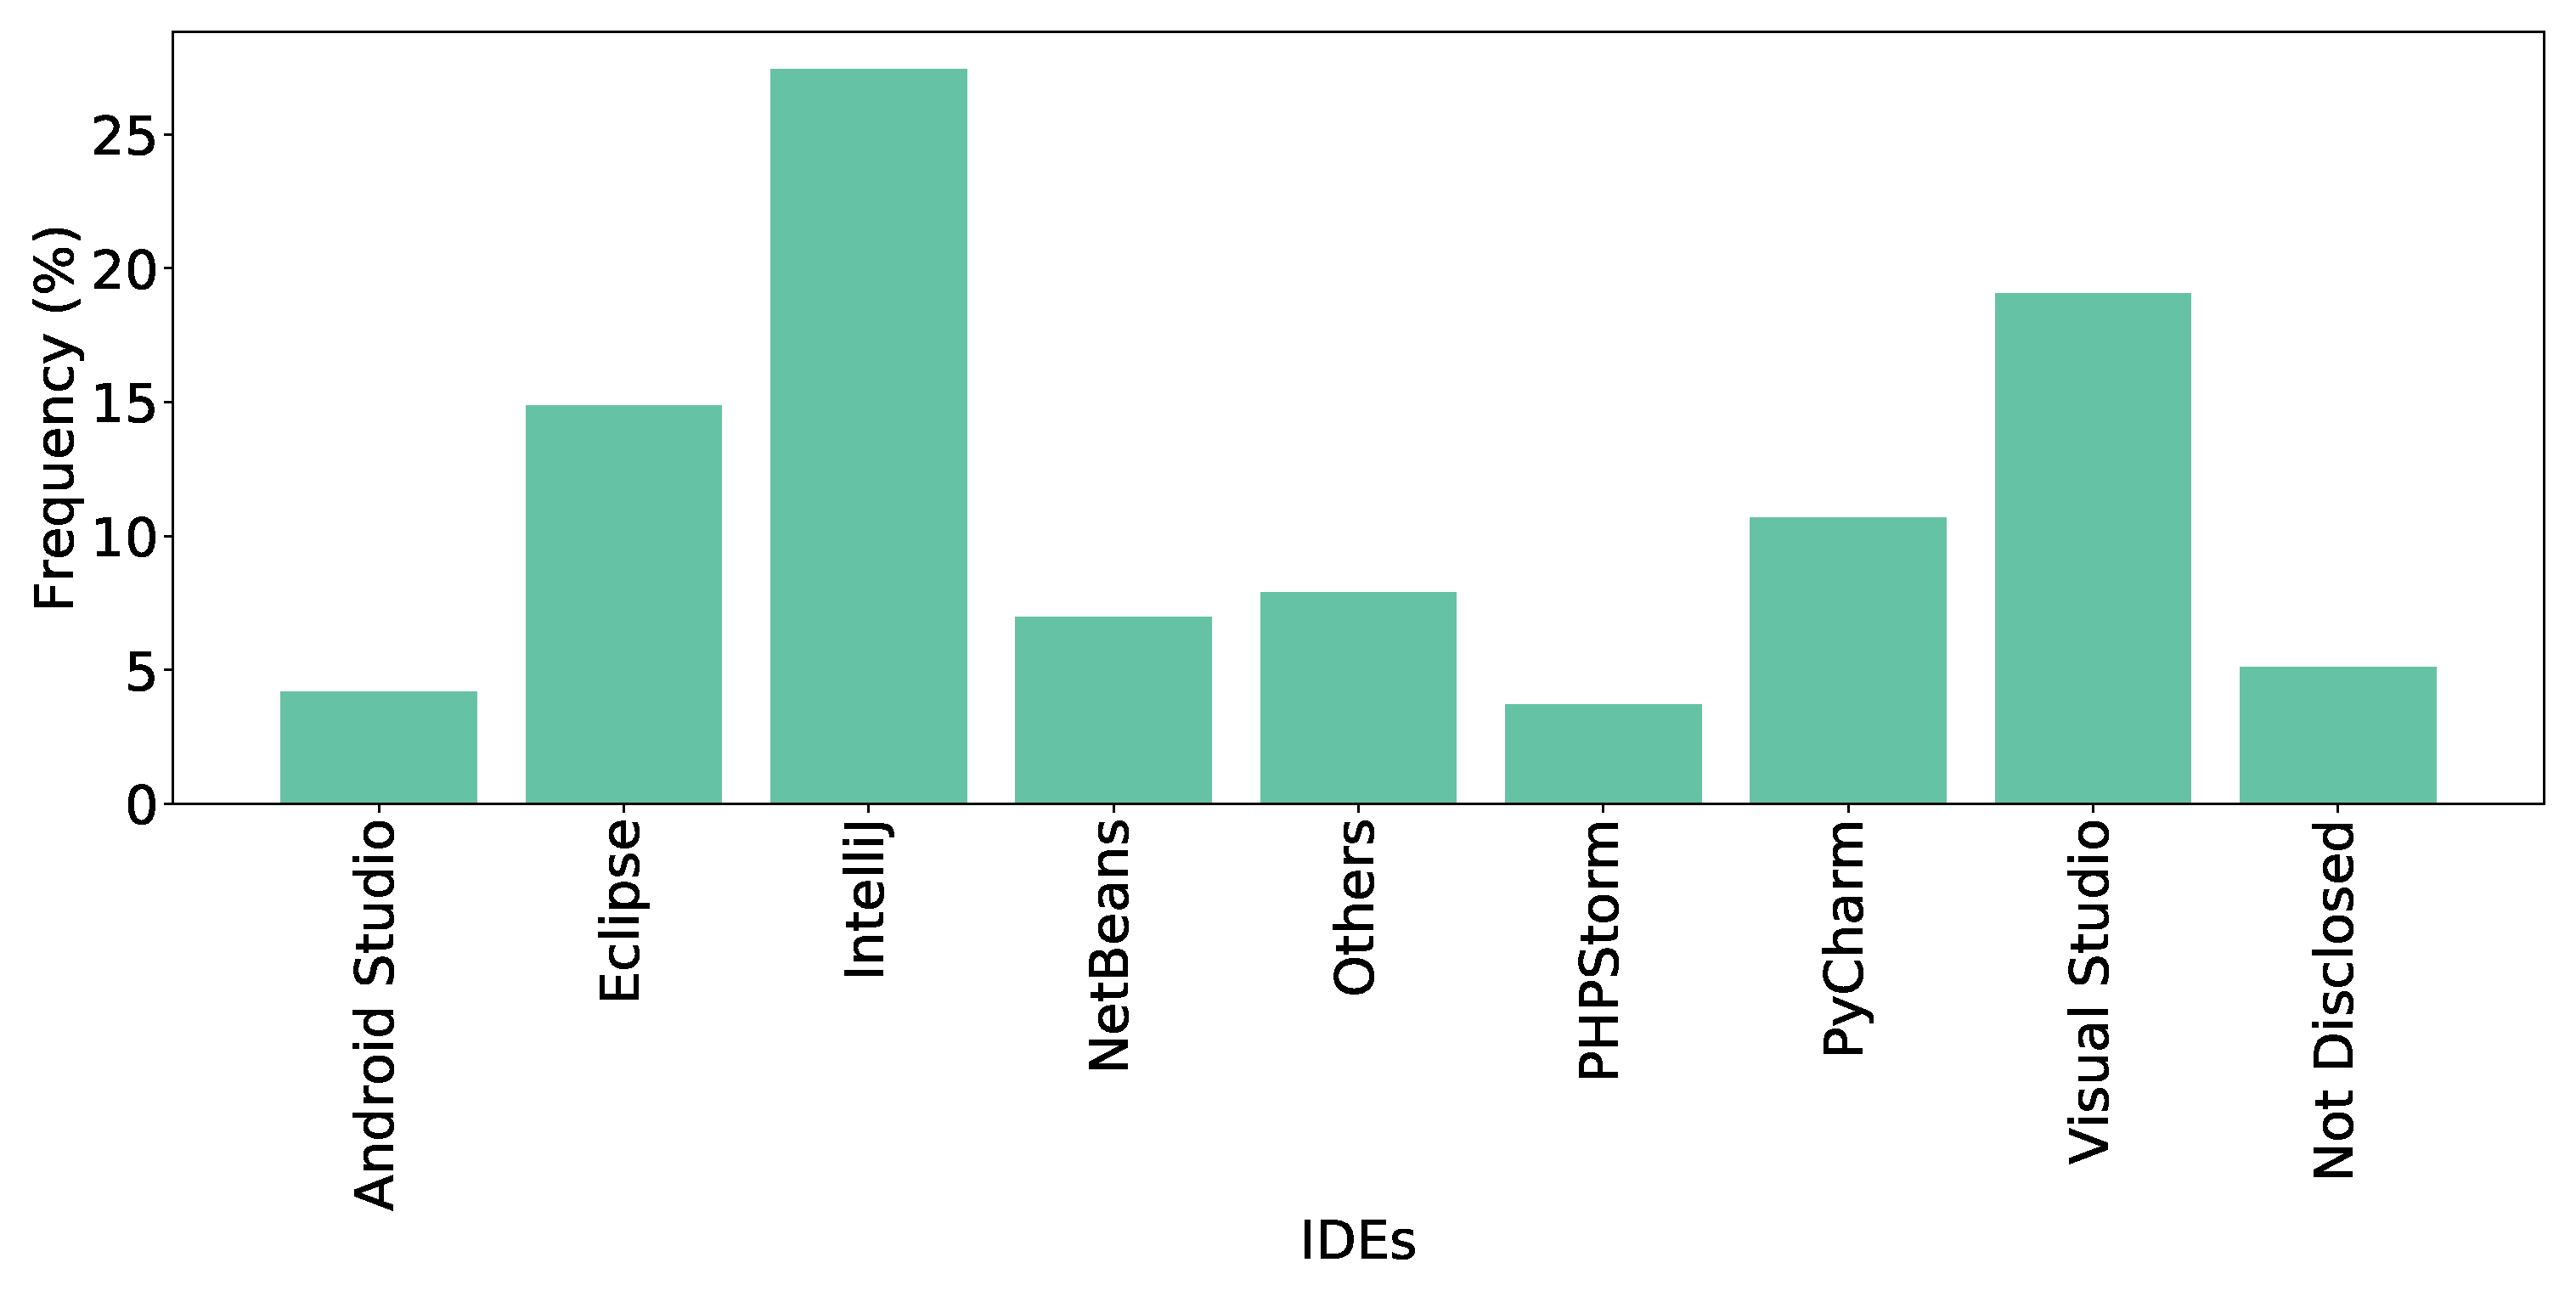
\includegraphics[width=0.8\textwidth]{Figures/Respondents_IDEs}
  \caption{IDE's}
  \label{fig:IDEs}
\end{figure}

\subsection{RQ3: What type of testing and deployment practices are used?}
\label{RQ3}
Testing is an important process in improving the quality of the software product. The purpose of this process is to find errors, which might occur during specification, design and code generation. Here we report the following results next:
\begin{itemize}
\item Software Testing Practices (Q 14)
\item Level of Automated Testing (Q 15)
\item Tools Used in Testing and QA (Q 16)
\item Continuous Deployment tools (Q 17)
\item Version Control (Q 18)
\end{itemize}

\subsubsection{Software Testing Practices}
According to \cref{fig:testing}, several number of testing practices are used during software development. The results show most of the organizations carried out unit testing (53\%), functional testing (49\%), user acceptance testing (39\%), GUI testing (31\%) etc.
\begin{figure}[htbp]
\centering
  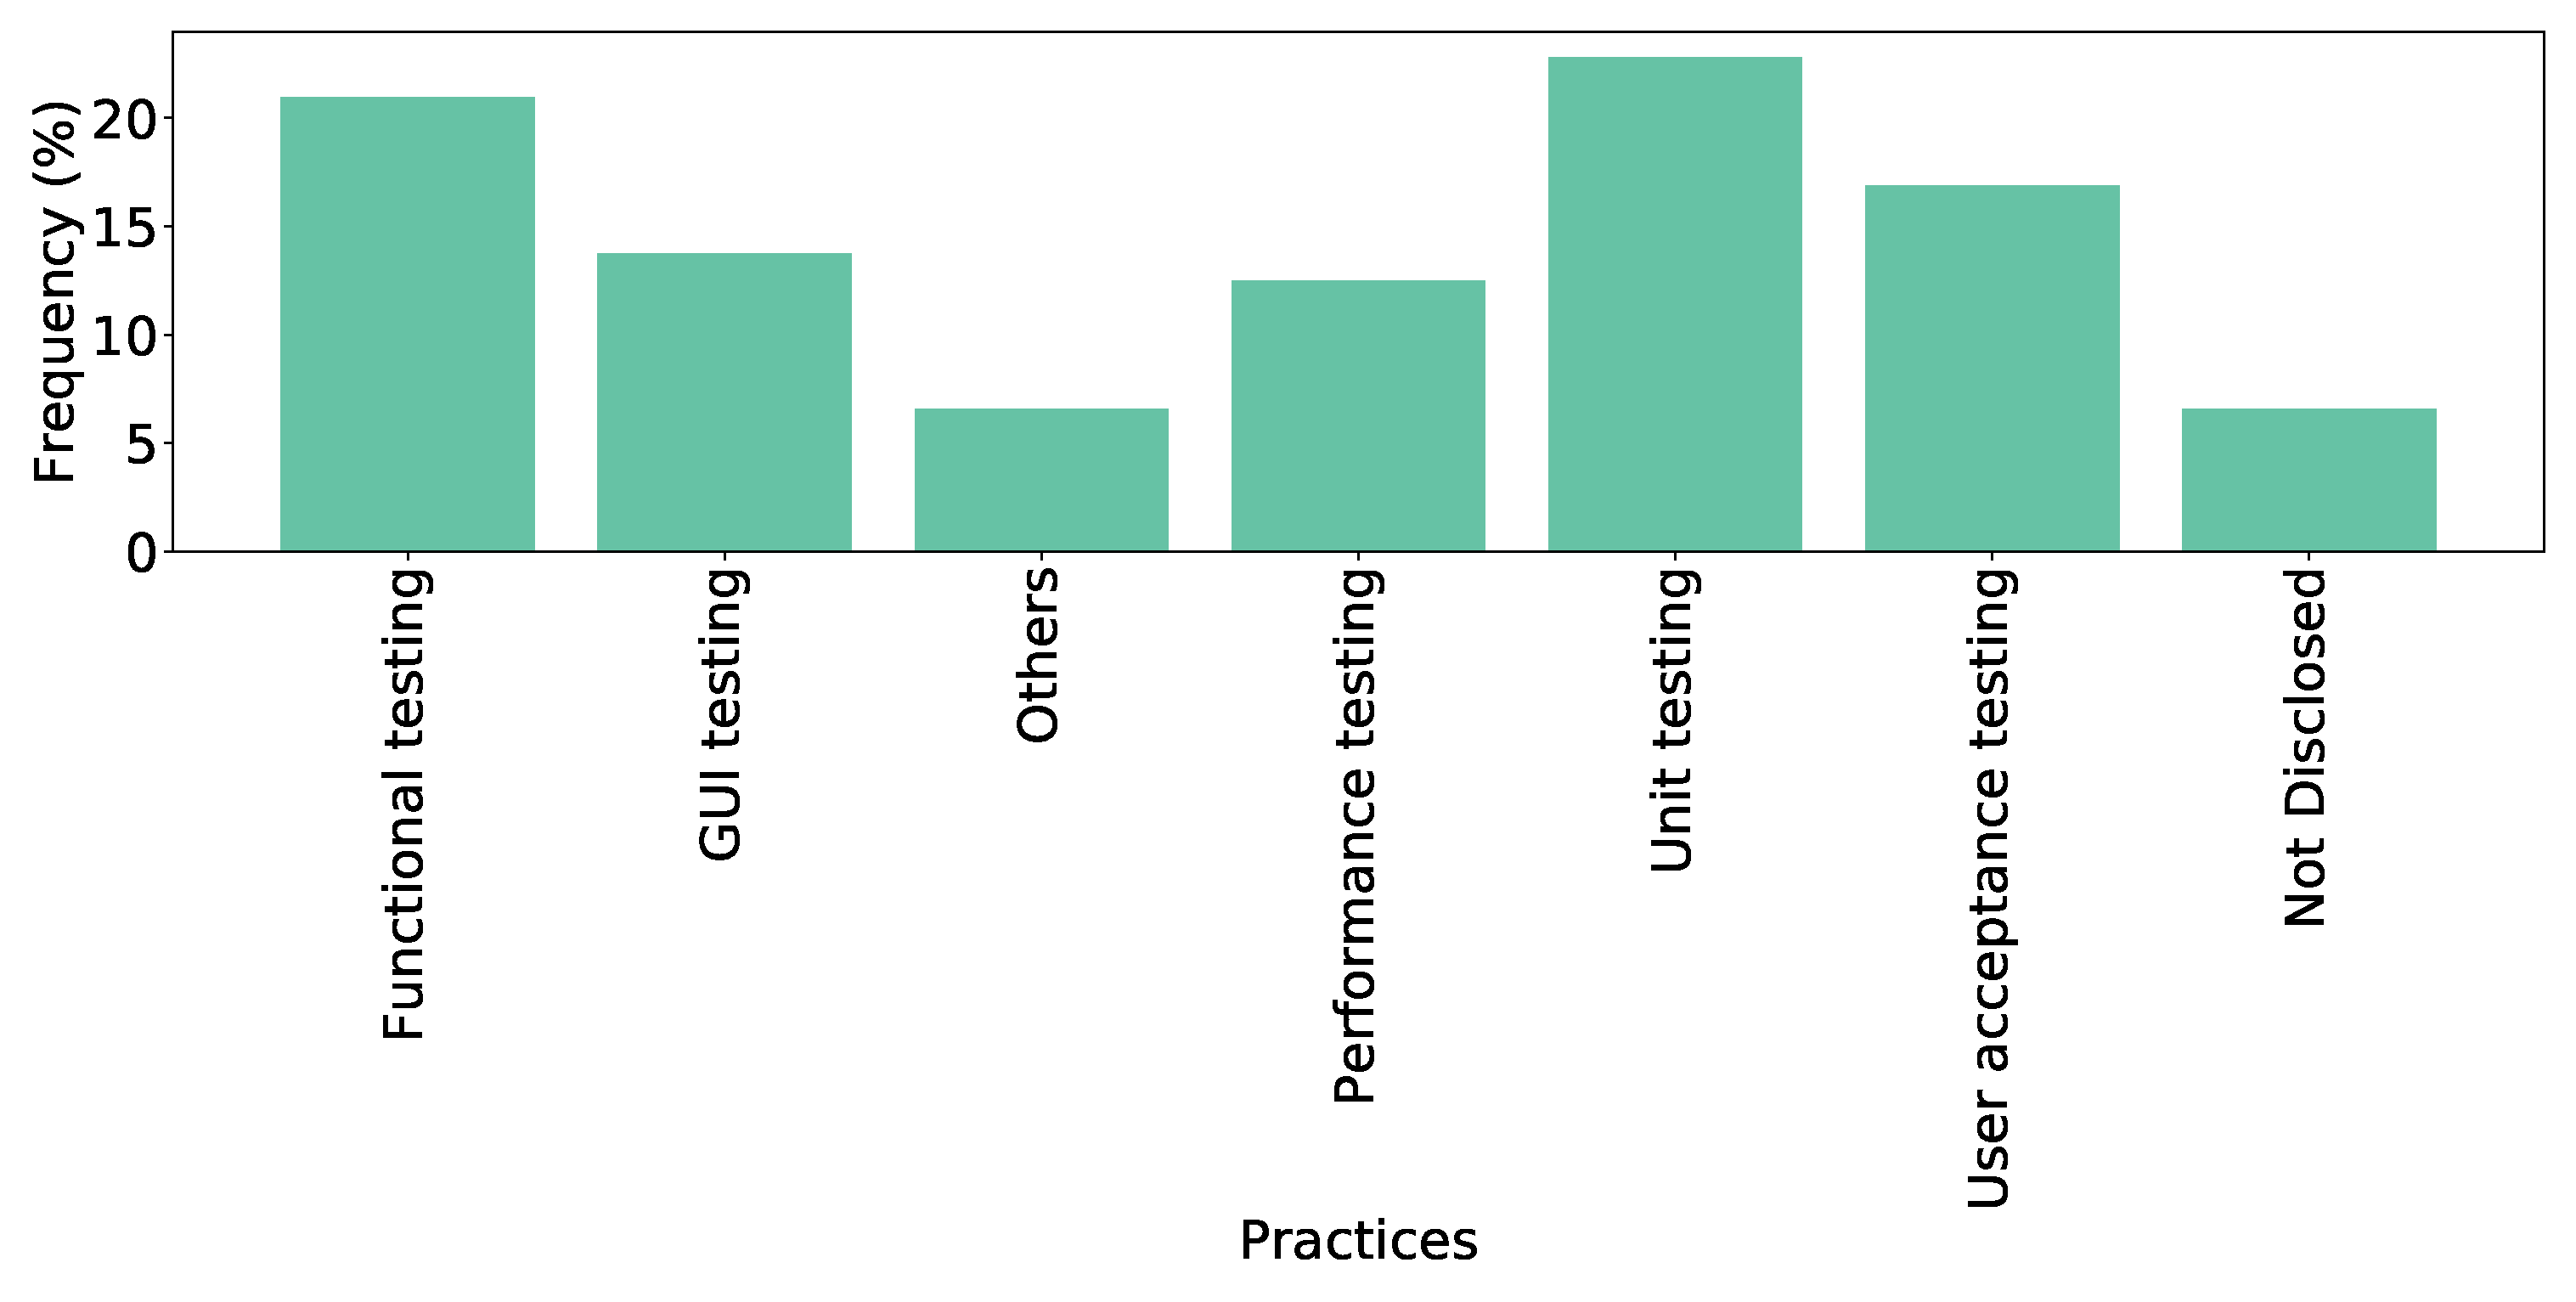
\includegraphics[width=0.8\textwidth]{Figures/Respondents_testing_practices}
  \caption{Testing Practices}
  \label{fig:testing}
\end{figure}

\subsubsection{Level of Automated Testing}
Question 15 asked about the level of automated testing. The responses were gathered using the Likert scale. This denotes that different respondents have very different practices in this context, i.e., some heavily practice automated testing, while others favor manual testing. Results are shown in \cref{fig:autoTest}.
\begin{figure}[htbp]
\centering
  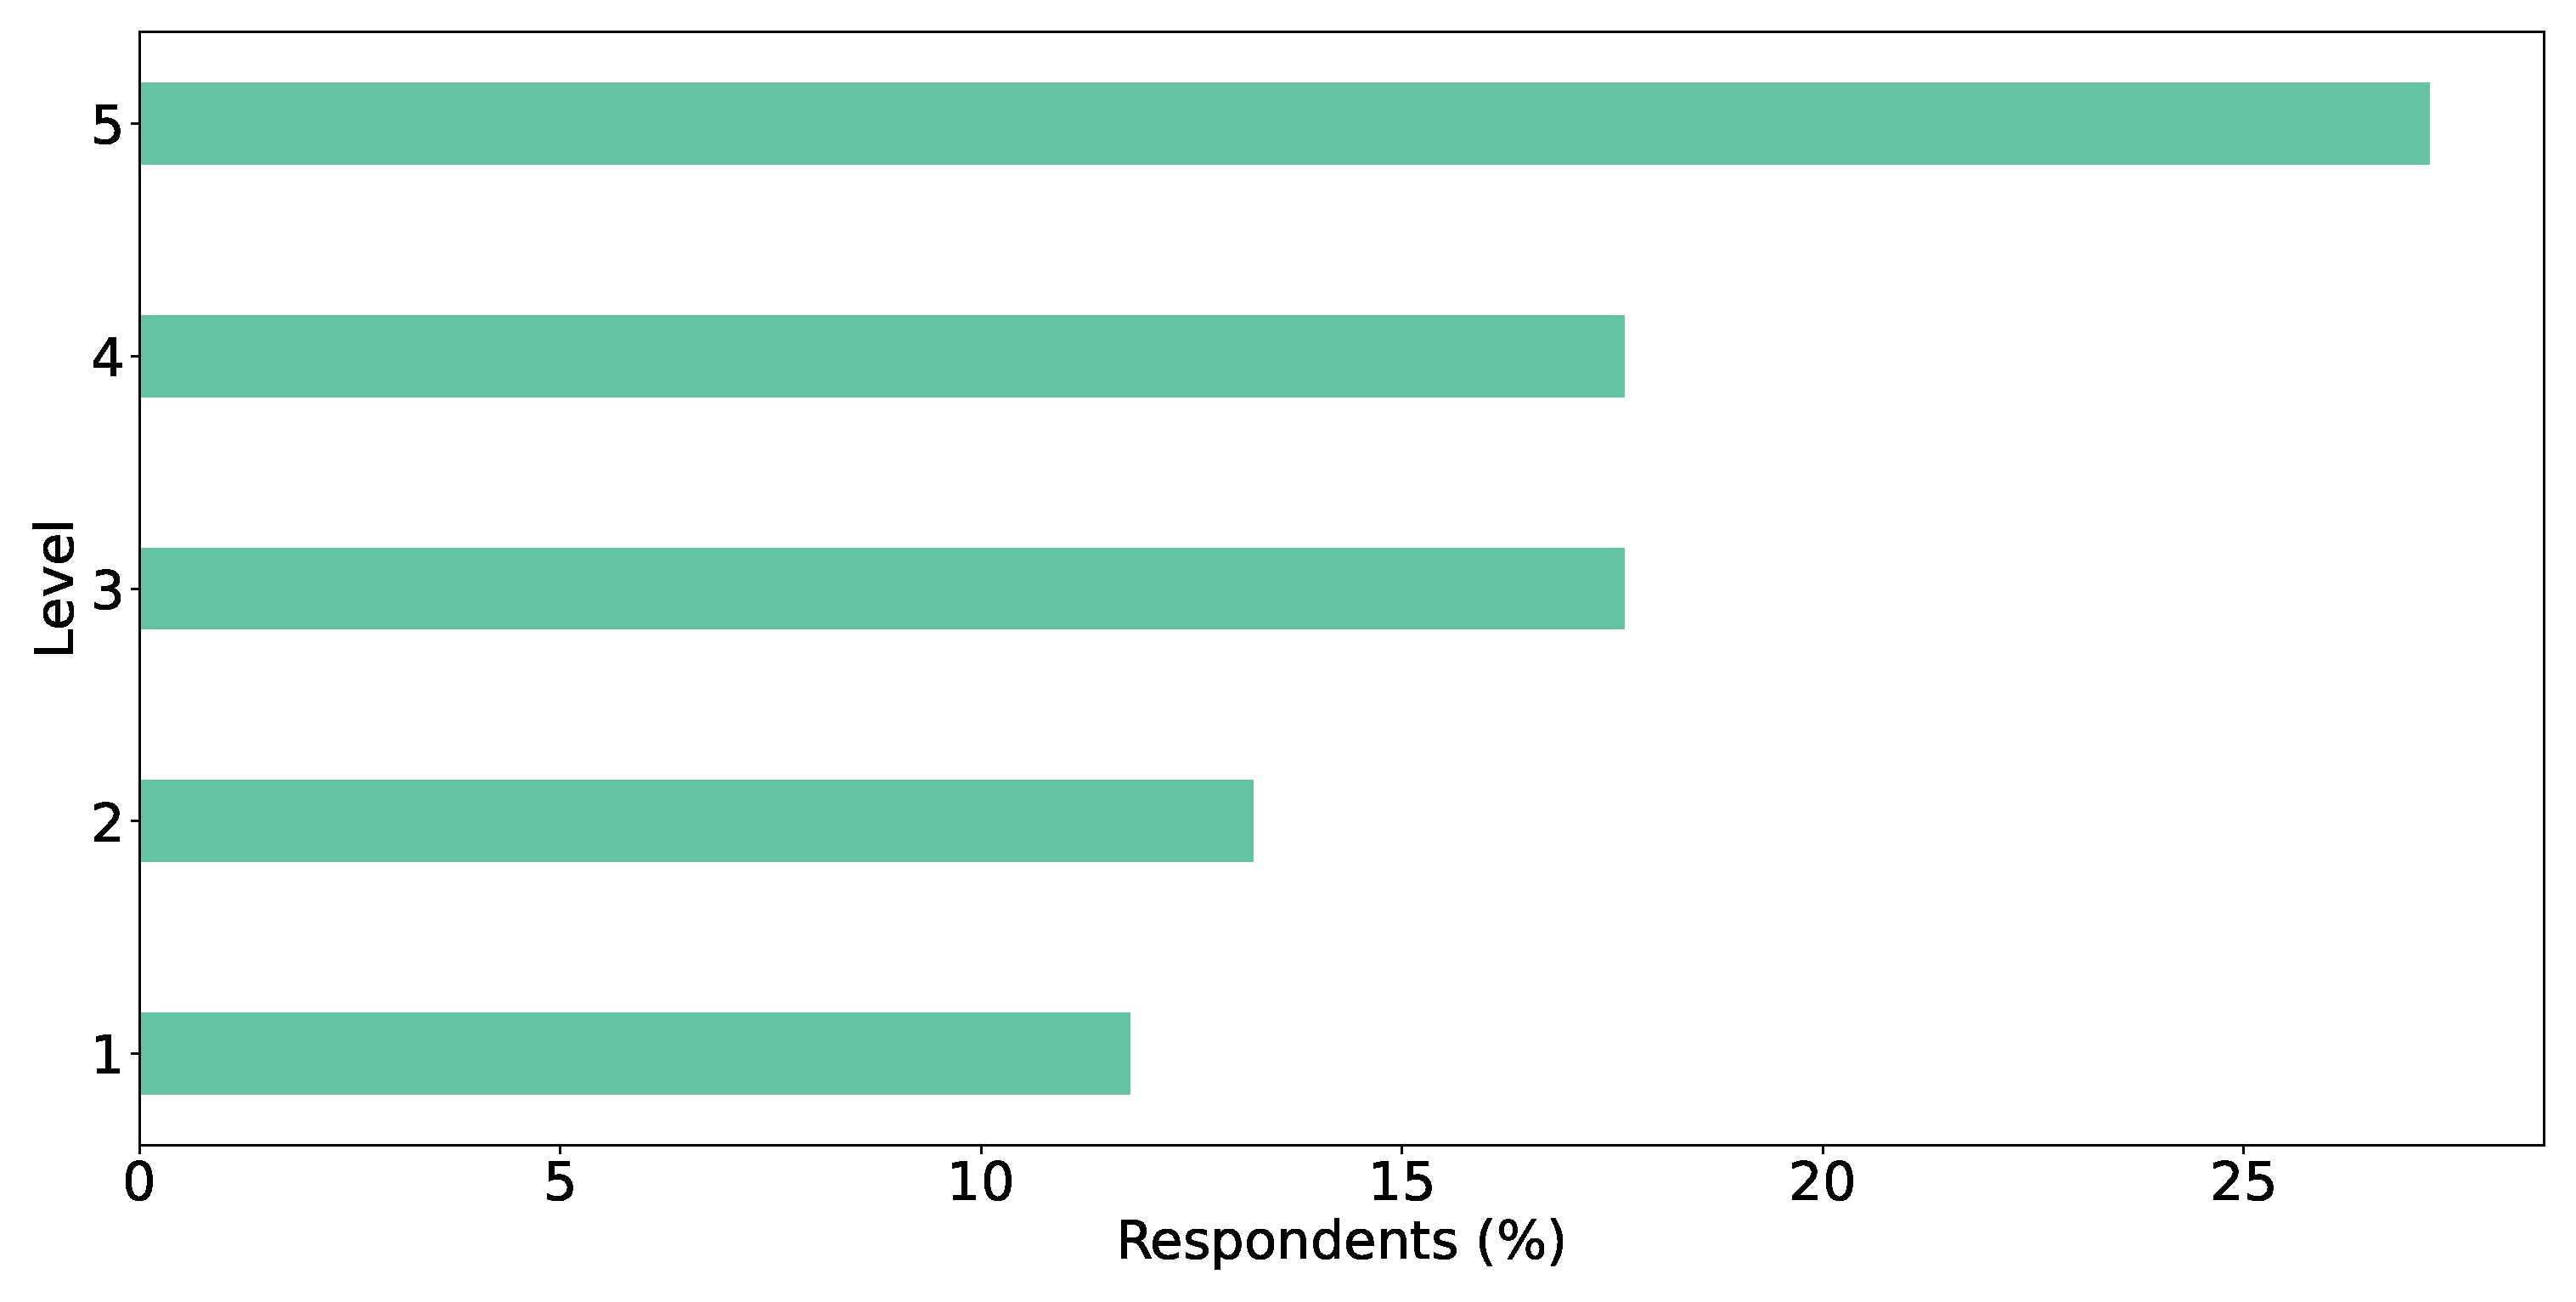
\includegraphics[width=0.8\textwidth]{Figures/Respondents_autotest_level}
  \caption{Automated Testing Level}
  \label{fig:autoTest}
\end{figure}

\subsubsection{Tools Used in Testing and QA}
Q 16 asked about the tools used in testing and quality assurance. According to \cref{fig:testingTools}, we see that most of the respondents have been used XUnit( eg, JUnit, NUnit) (30\%), selenium (27\%), Jenkins (20\%), others (9\%). 
\begin{figure}[htbp]
\centering
  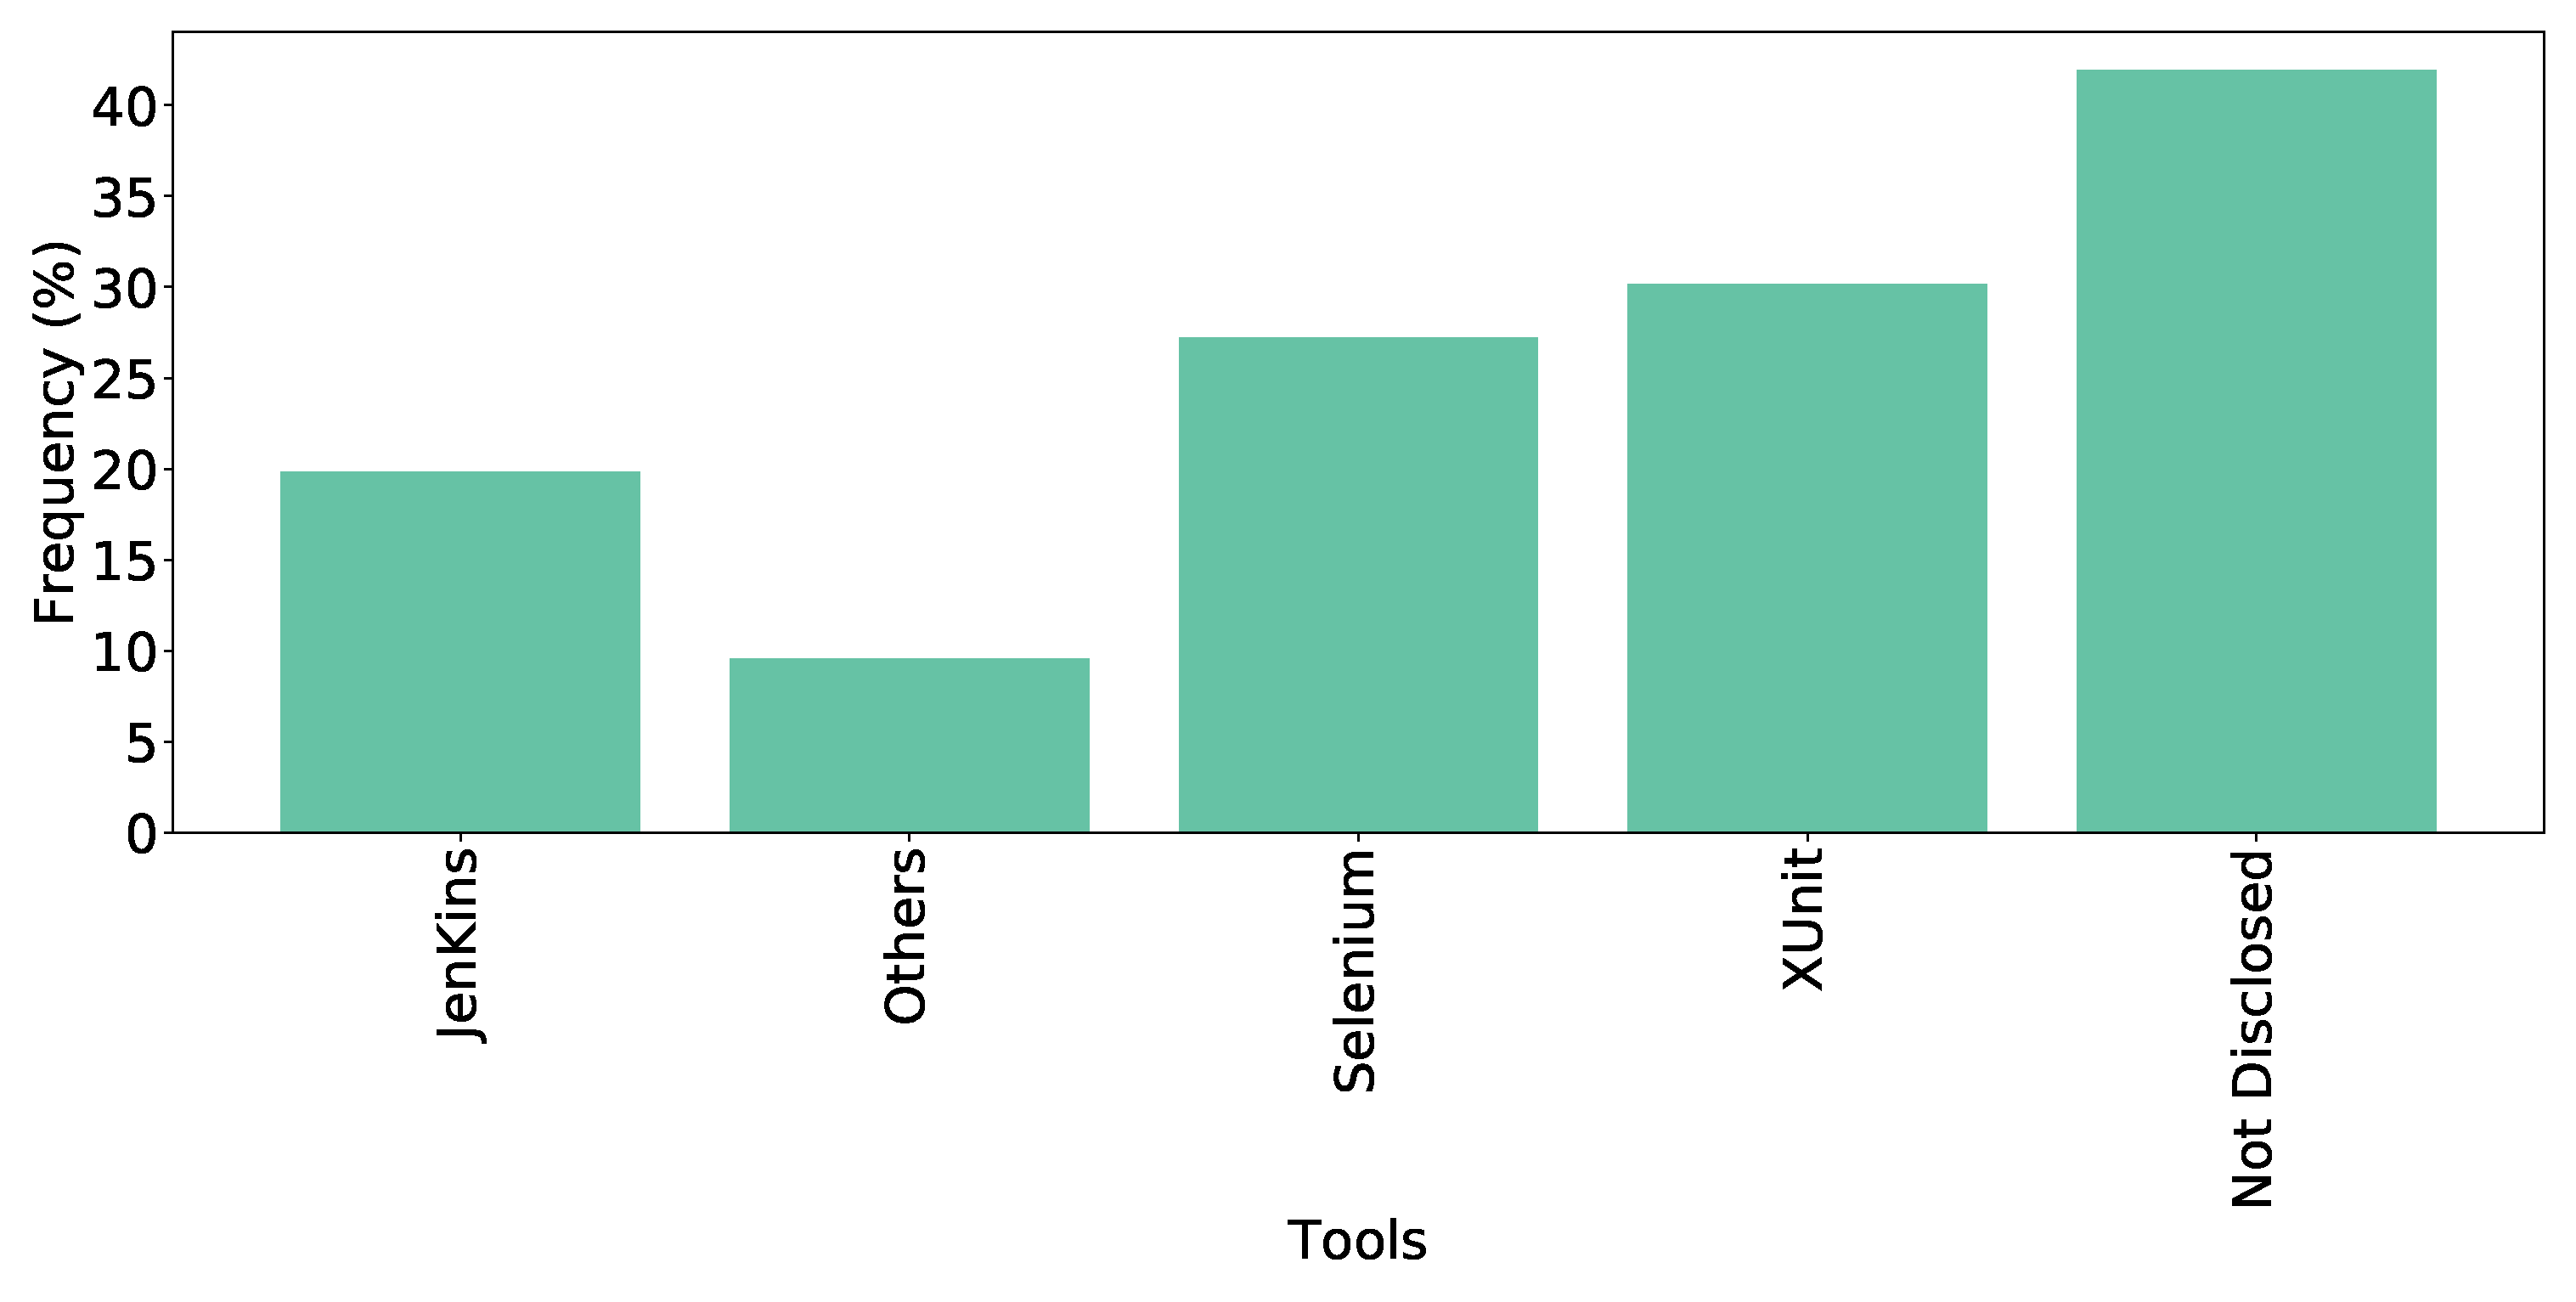
\includegraphics[width=0.8\textwidth]{Figures/Respondents_testing_tools}
  \caption{Testing \& QA Tools}
  \label{fig:testingTools}
\end{figure}

\subsubsection{Deployment Tools}
According to \cref{fig:deployTools}, wee see that most of the respondents use AWS code-deploy (12\%) and JenKins (12\%). The other deployment tools are Bamboo (5\%), teamcity (4\%), octopus (2\%). Respondents voted none (4\%) as they didn’t use any deployment tools.
\begin{figure}[htbp]
\centering
  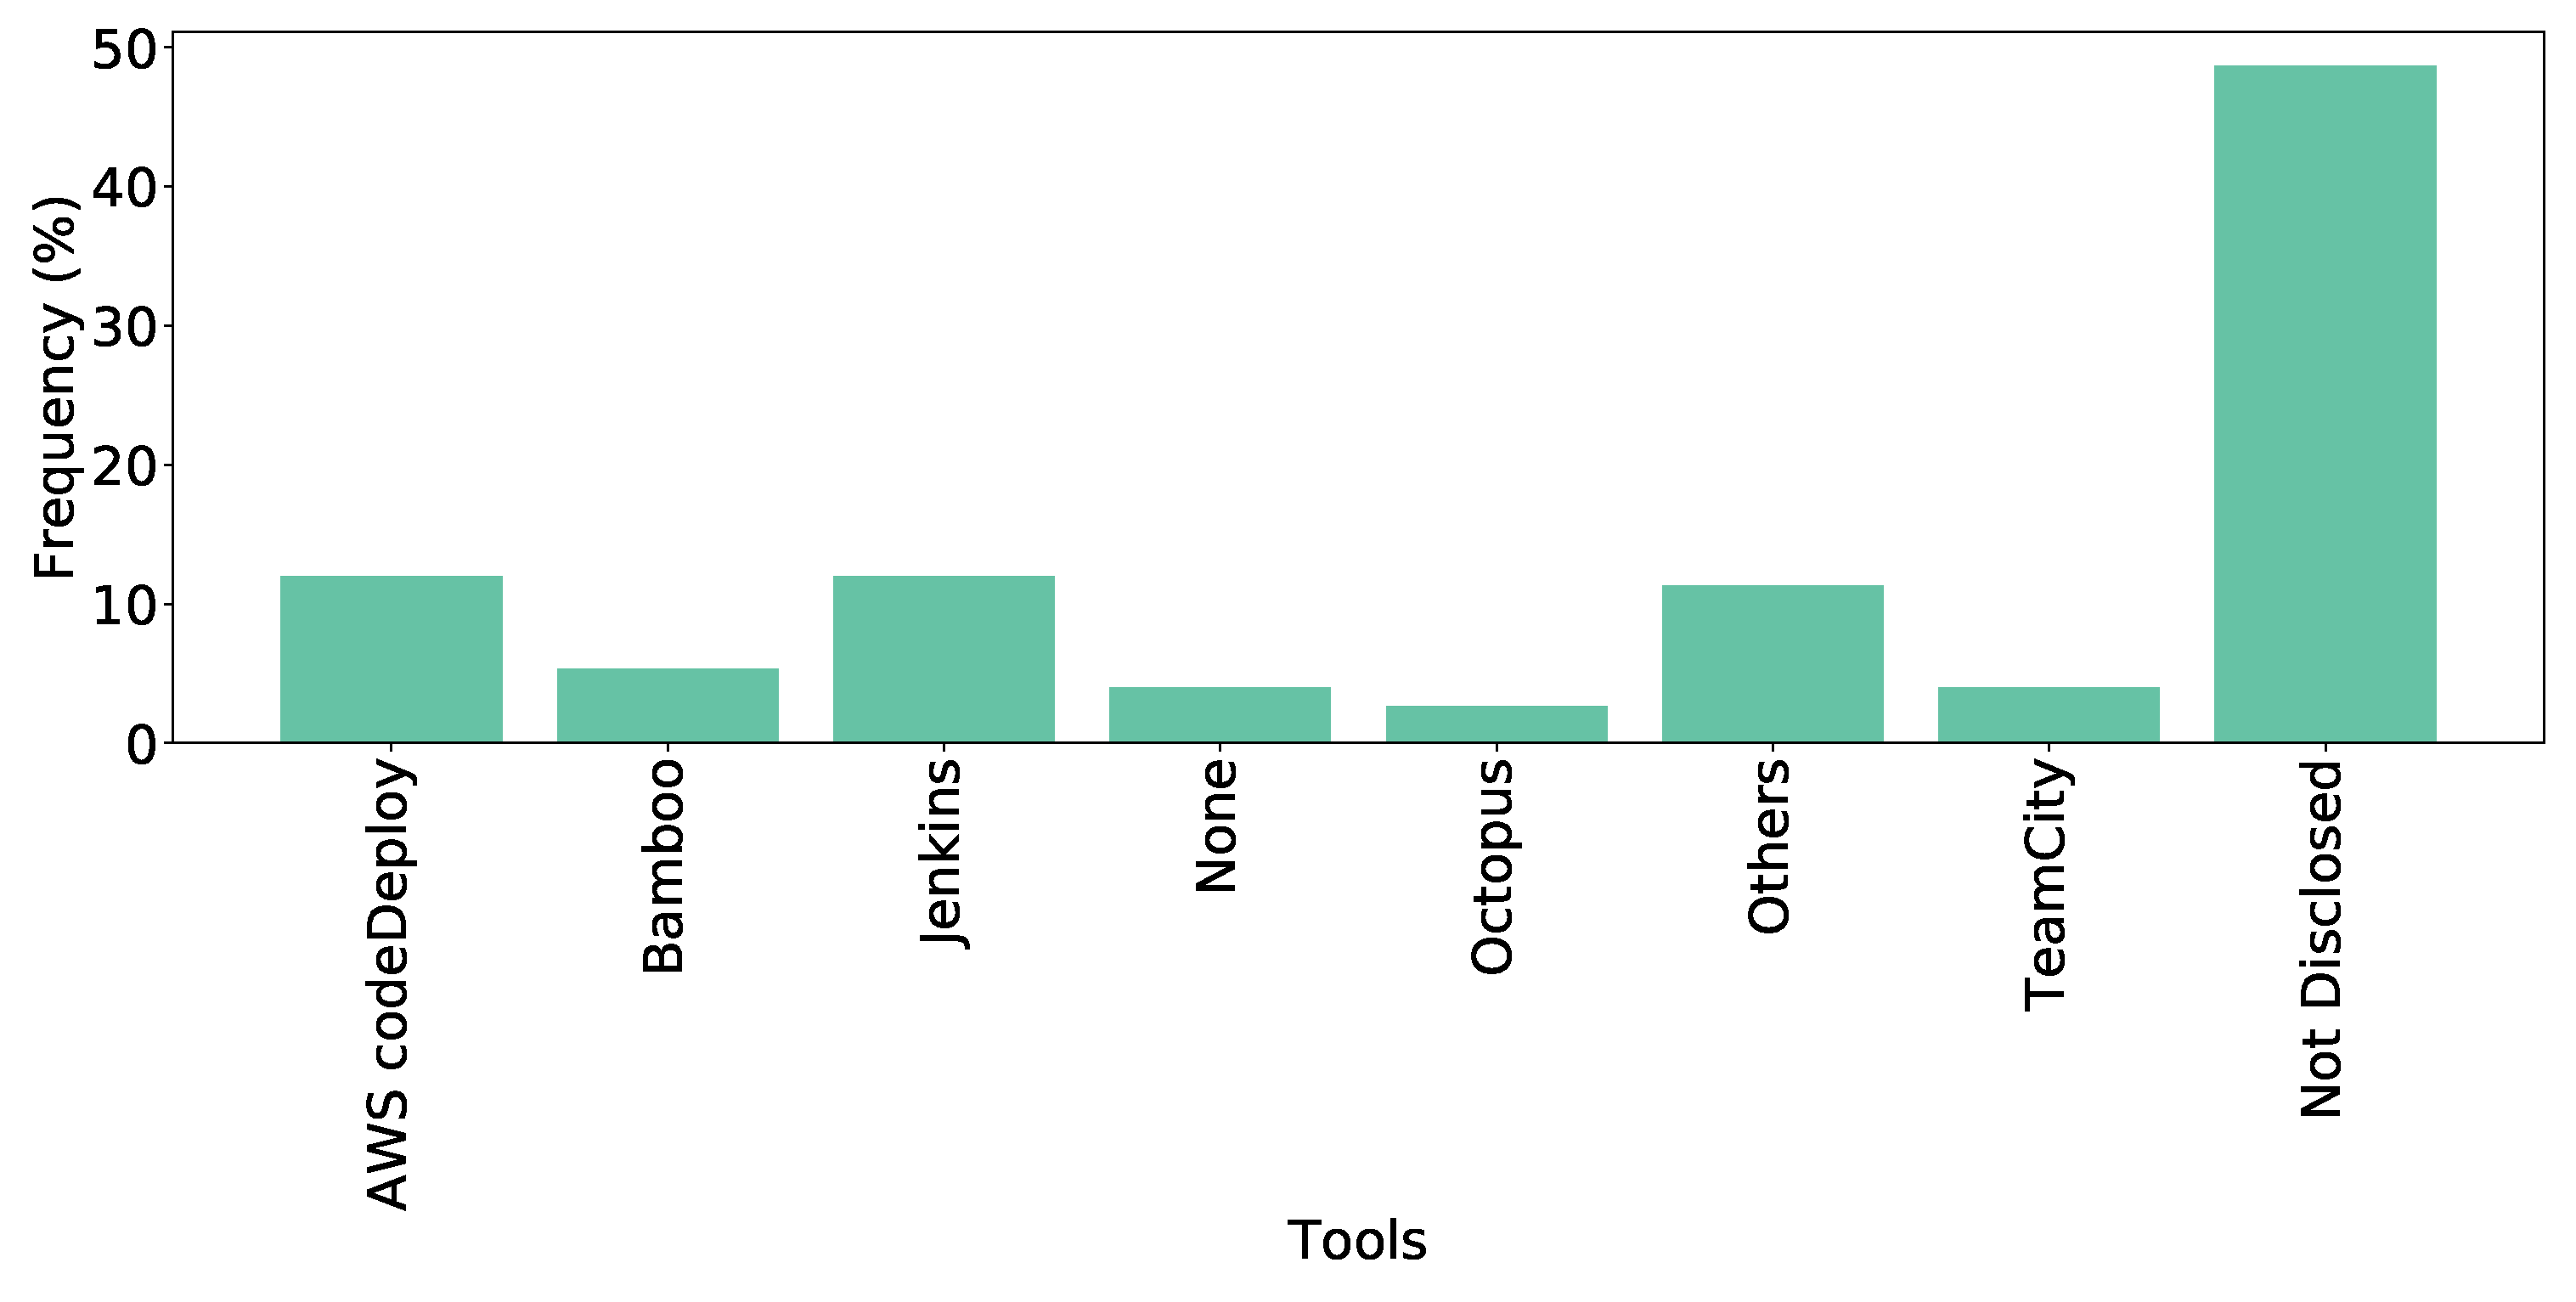
\includegraphics[width=0.8\textwidth]{Figures/Respondents_deployment_tools}
  \caption{Deployment Tools}
  \label{fig:deployTools}
\end{figure}

\subsubsection{Version Control}
\hfill\\
Respondents were allowed to select more than one option. As shown in figure \ref{fig:versionControl}, Git (78\%) and BitBucket (29\%) are mostly-used version control in the software industry. Beside these SVN (5\%), others (4\%) are used.  The 2018 Stack overflow survey\citep{StackoverflowSurvey2018} reports that  the most popular version control system is Git (87.2\% developer uses Git) and the second most popular is SVN (16.1\% developer uses SVN). However, in our survey, we found slightly different result,the most popular version control system is Git and the second most popular is Bitbucket. This might be related  to the declining popularity of SVN over the years. From the Stack overflow survey over the range 2017-2019, it is clear that SVN is losing popularity to Git. Nowadays, SVN is mainly used for versioning legacy projects. As the SE industry of Bangladesh is quite new, we observe such discrepancy in the popularity of SVN.

\begin{figure}[htbp]
\centering
  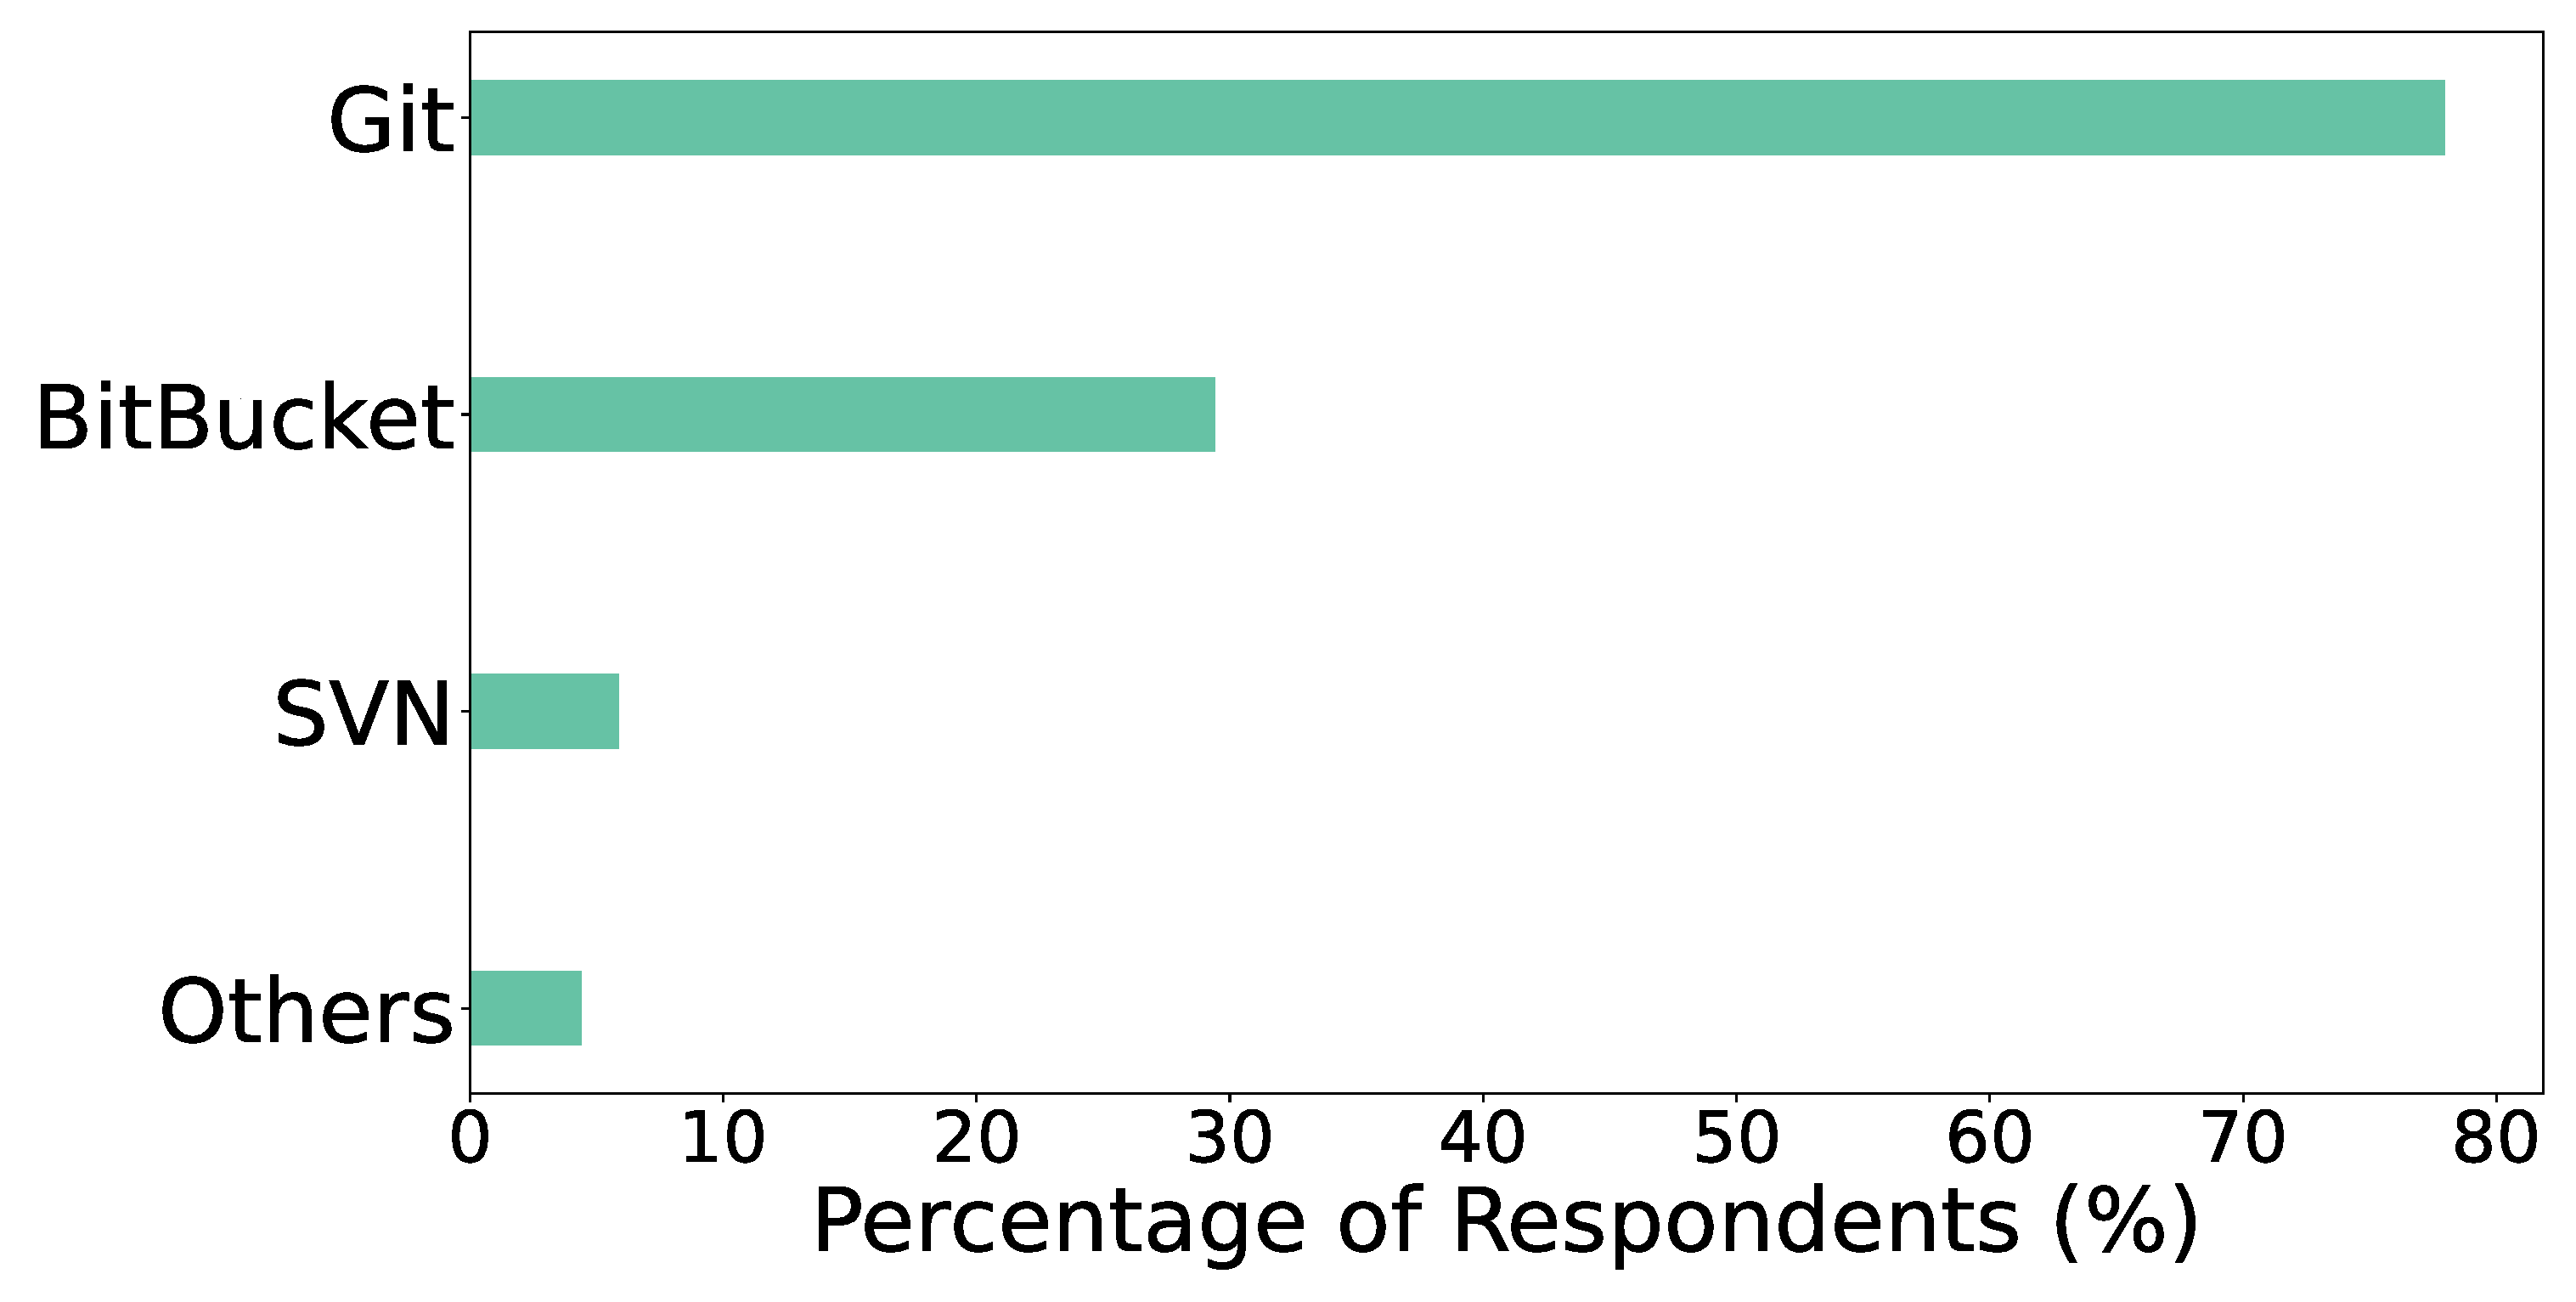
\includegraphics[width=0.8\textwidth]{Figures/Respondents_version_control}
  \caption{Version Control}
  \label{fig:versionControl}
\end{figure}
\subsection{RQ4: How are the security and performance is ensured in a product of a company?}
\label{RQ4}
This particular question covers how a company secures its code from external attack and maintain its performance after deployment. It also slightly deals with the problem of scalability. Performance depends greatly on whether a product has scalability or not. So, we will cover the following points here:
\begin{itemize}
    \item Security
    \item Performance
    \item Scalability
\end{itemize}
\subsubsection{Security}
\label{Security}
\begin{figure}[htbp]
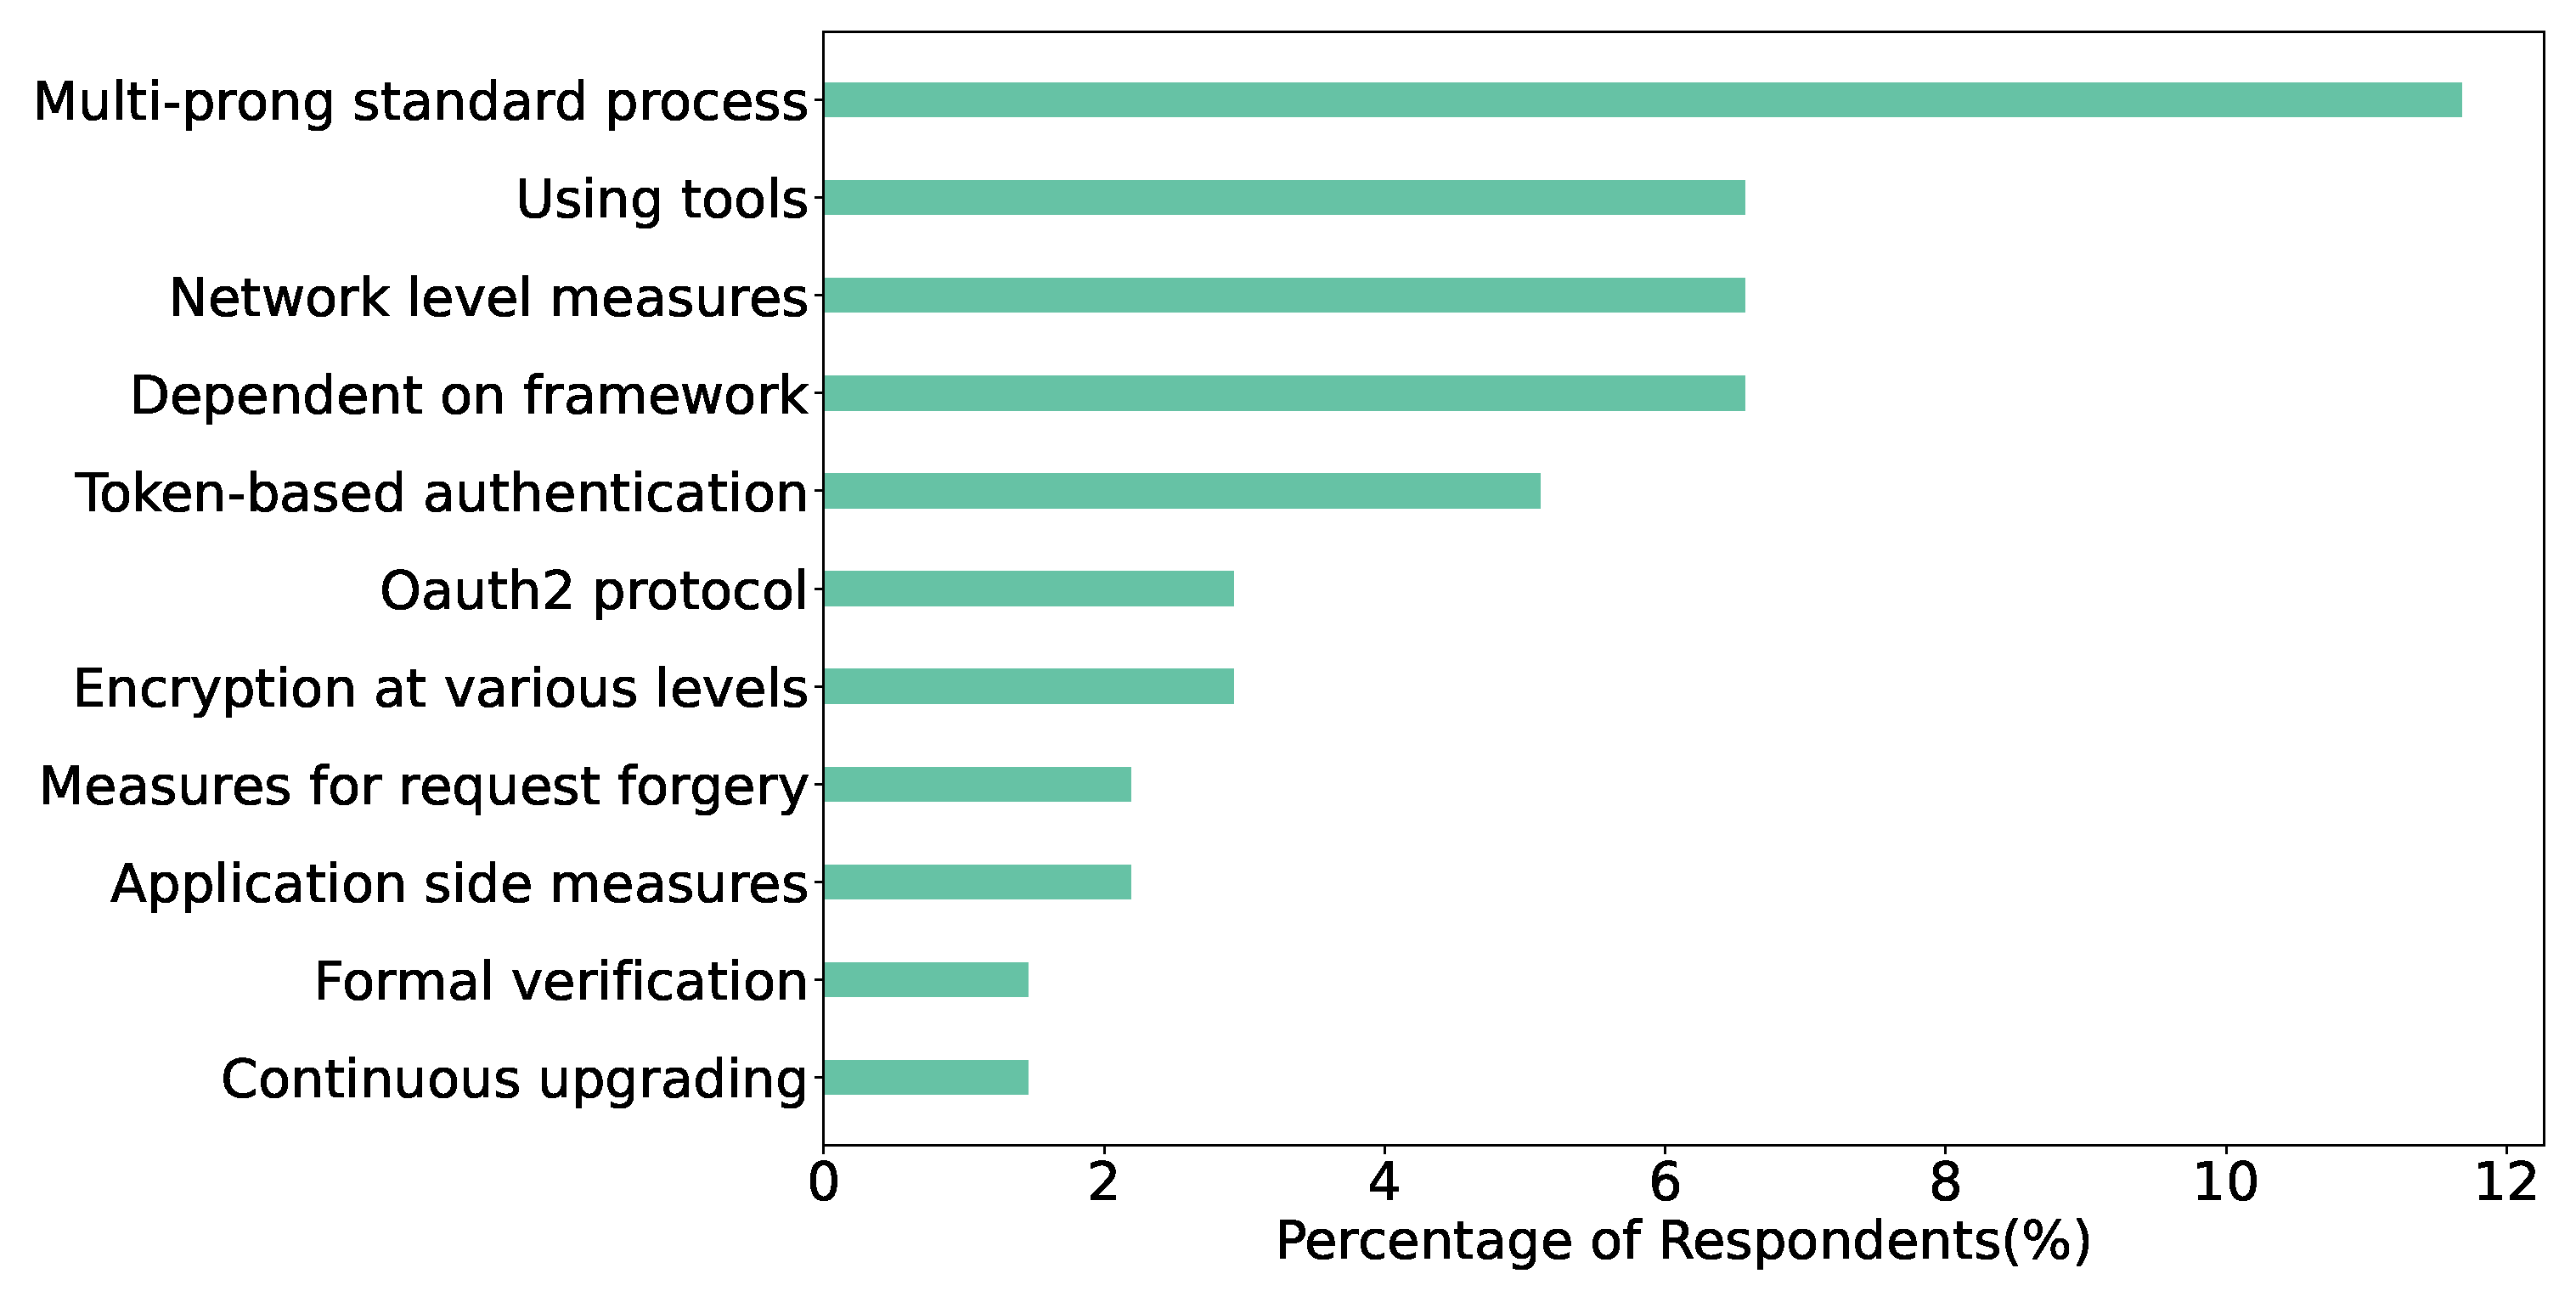
\includegraphics[scale=0.28]{Figures/Security.eps} 
\caption{Measures to maintain security of products}
\label{fig:Measures to ensure security}
\end{figure}
\hfill\\
Security refers to confidentiality, integrity and authenticity. To maintain security of software product SE industry of Bangladesh is mainly dependent on Standard process which includes cloud based security, third party software, OS hardening followed by uses of security tools, network level measures and framework security. As found by Harrison et al.\cite{Harrison2010} network level measures are the first choice in ensuring security of software product which matches with our findings. Srinivasan et al.\cite{Srinivasan2017} listed top 10 web framework in terms of security testing where Spring framework achieved 7\textsuperscript{th} position. From figure ~\ref{fig:frameworks} we have seen that most of our respondents use Spring framework for software development. This might be the reason that a lot number of respondents dependent on framework for ensuring security.
\begin{enumerate}

    \item \textbf{Application Side Measures}: Security is ensured at the software or application side. 2.19\% respondents implemented security measures at application level.
    \surveyquote{At application level, could not achieve others yet}{72}
    
    \item \textbf{Server Side Measures}: Security is ensured at the server side. 0.73\% respondents implemented security measures at server level.
    \surveyquote{We use github/bitbucket repository systems to code maintain and store. We use server side security on AWS and other third party server host.}{48}
    
    \item \textbf{Network level Measures}: Network level measures include IP-white-listing, port-blocking, VPN and  use of HTTPS  in software. 6.57\% respondents use at least one of the before mentioned strategy to ensure security.
    \surveyquote{network blocking and common security measures}{2}
    
    \item \textbf{Formal Verification}: Security threats can be mitigated by  a code level review . 1.46\% respondents ensured the practice of formal code review
    \surveyquote{There are some basic guidelines that we must follow and while code review this needs to be an absolute part that needs to be checked before the code gets merged}{112}
    
    \item \textbf{Measures for request forgery}: Measures against cross site forgery is implemented to ensure security. This includes CORS or cross origin resource sharing, CSRF or cross site request forgery or one click attack or XSRF. 2.19\% respondents implemented measures agianst  Cross-site request forgery to ensure security.
    \surveyquote{Security testings like: SQL injection, cross-site scripting, CSRF, API security, use of https,  detecting malicious / suspicious HTTP requests and auto-blocking}{42}

    \item \textbf{OAuth 2.0} : OAuth 2.0 is the industry-standard protocol for authorization. OAuth 2.0 focuses on client developer simplicity while providing specific authorization flows for web applications, desktop applications, mobile phones, and living room devices. Many (2.92\%) respondents use OAuth 2.0 protocol as the main way of maintaining security.
    \surveyquote{OAuth 2.0, JWT, Token Base Authentication, CORS Filter, XSRF}{127}
    
    \item \textbf{Token-based authentication} : A token-based authentication system allows users to enter their username and password in order to obtain a token which allows them to fetch a specific resource - without using their username and password. Once their token has been obtained, the user can offer the token which offers access to a specific resource for a time period - to the remote site. 5.11\% people expressed its eligibility.
    \surveyquote{Token based authentication for all of my rest service}{80}
    
    \item \textbf{Multi-prong Standard Process} : Following multiprong standard processes is the best way to enforce security. About 10.22\% of the total respondents expressed this opinion.
    \surveyquote{Multi Prong Standard Processes and Products}{110}
    
    
    \item \textbf{Encryption at Various Levels} : Not only at password,but also in every level of software, encryption is first and foremost to ensure its security.
    \surveyquote{use encryption at different level of software (server, network, transmission layer, database and software layer.)}{35}
    
    \item \textbf{Use of tools} : Respondents use various open-source/ paid tools for scanning  and testing. These tools help to find security threats in an existing system. The tools includes OWASP based tools and  penetration testing tools
    \surveyquote{use encryption at different level of software (server, network, transmission layer, database and software layer.)}{35}
    
    
    \item \textbf{Dependent on Framework} : Common framework provides basic to intermediate level security measures in the application. 6.57\% respondents depends on framework for security. The framework includes spring and  HDIV.
    \surveyquote{https, popular framework which already prevents some type of attacks. rest of the things on case-by-case basis)}{79}
    
    
    \item \textbf{Non-disclosure agreement} : 2.19\% refused to provide any details due to non-disclosure agreement.
    \surveyquote{As we are regulated by Bangladesh Bank as a payment processing platform, we need to maintain certain security compliance which cannot be disclosed here. The security compliance is similar to the PCI DSS compliance which I can say}{10}
    
    \item \textbf{Continuous Upgrading}: As security threats are evolving thus current systems need continuous upgradation in a frequent interval. 1.46\% respondents said they arrange frequent hackathon, workshop, security audits to address the continuously evolving security threat.
    \surveyquote{We run security audit of our office environment. We also conduct security session per 6 months to introduce latest trend in threats and what we can do to avoid it}{57}
    

   
\end{enumerate}

\subsubsection{Performance}
\label{Performance}
\begin{figure}[htbp]
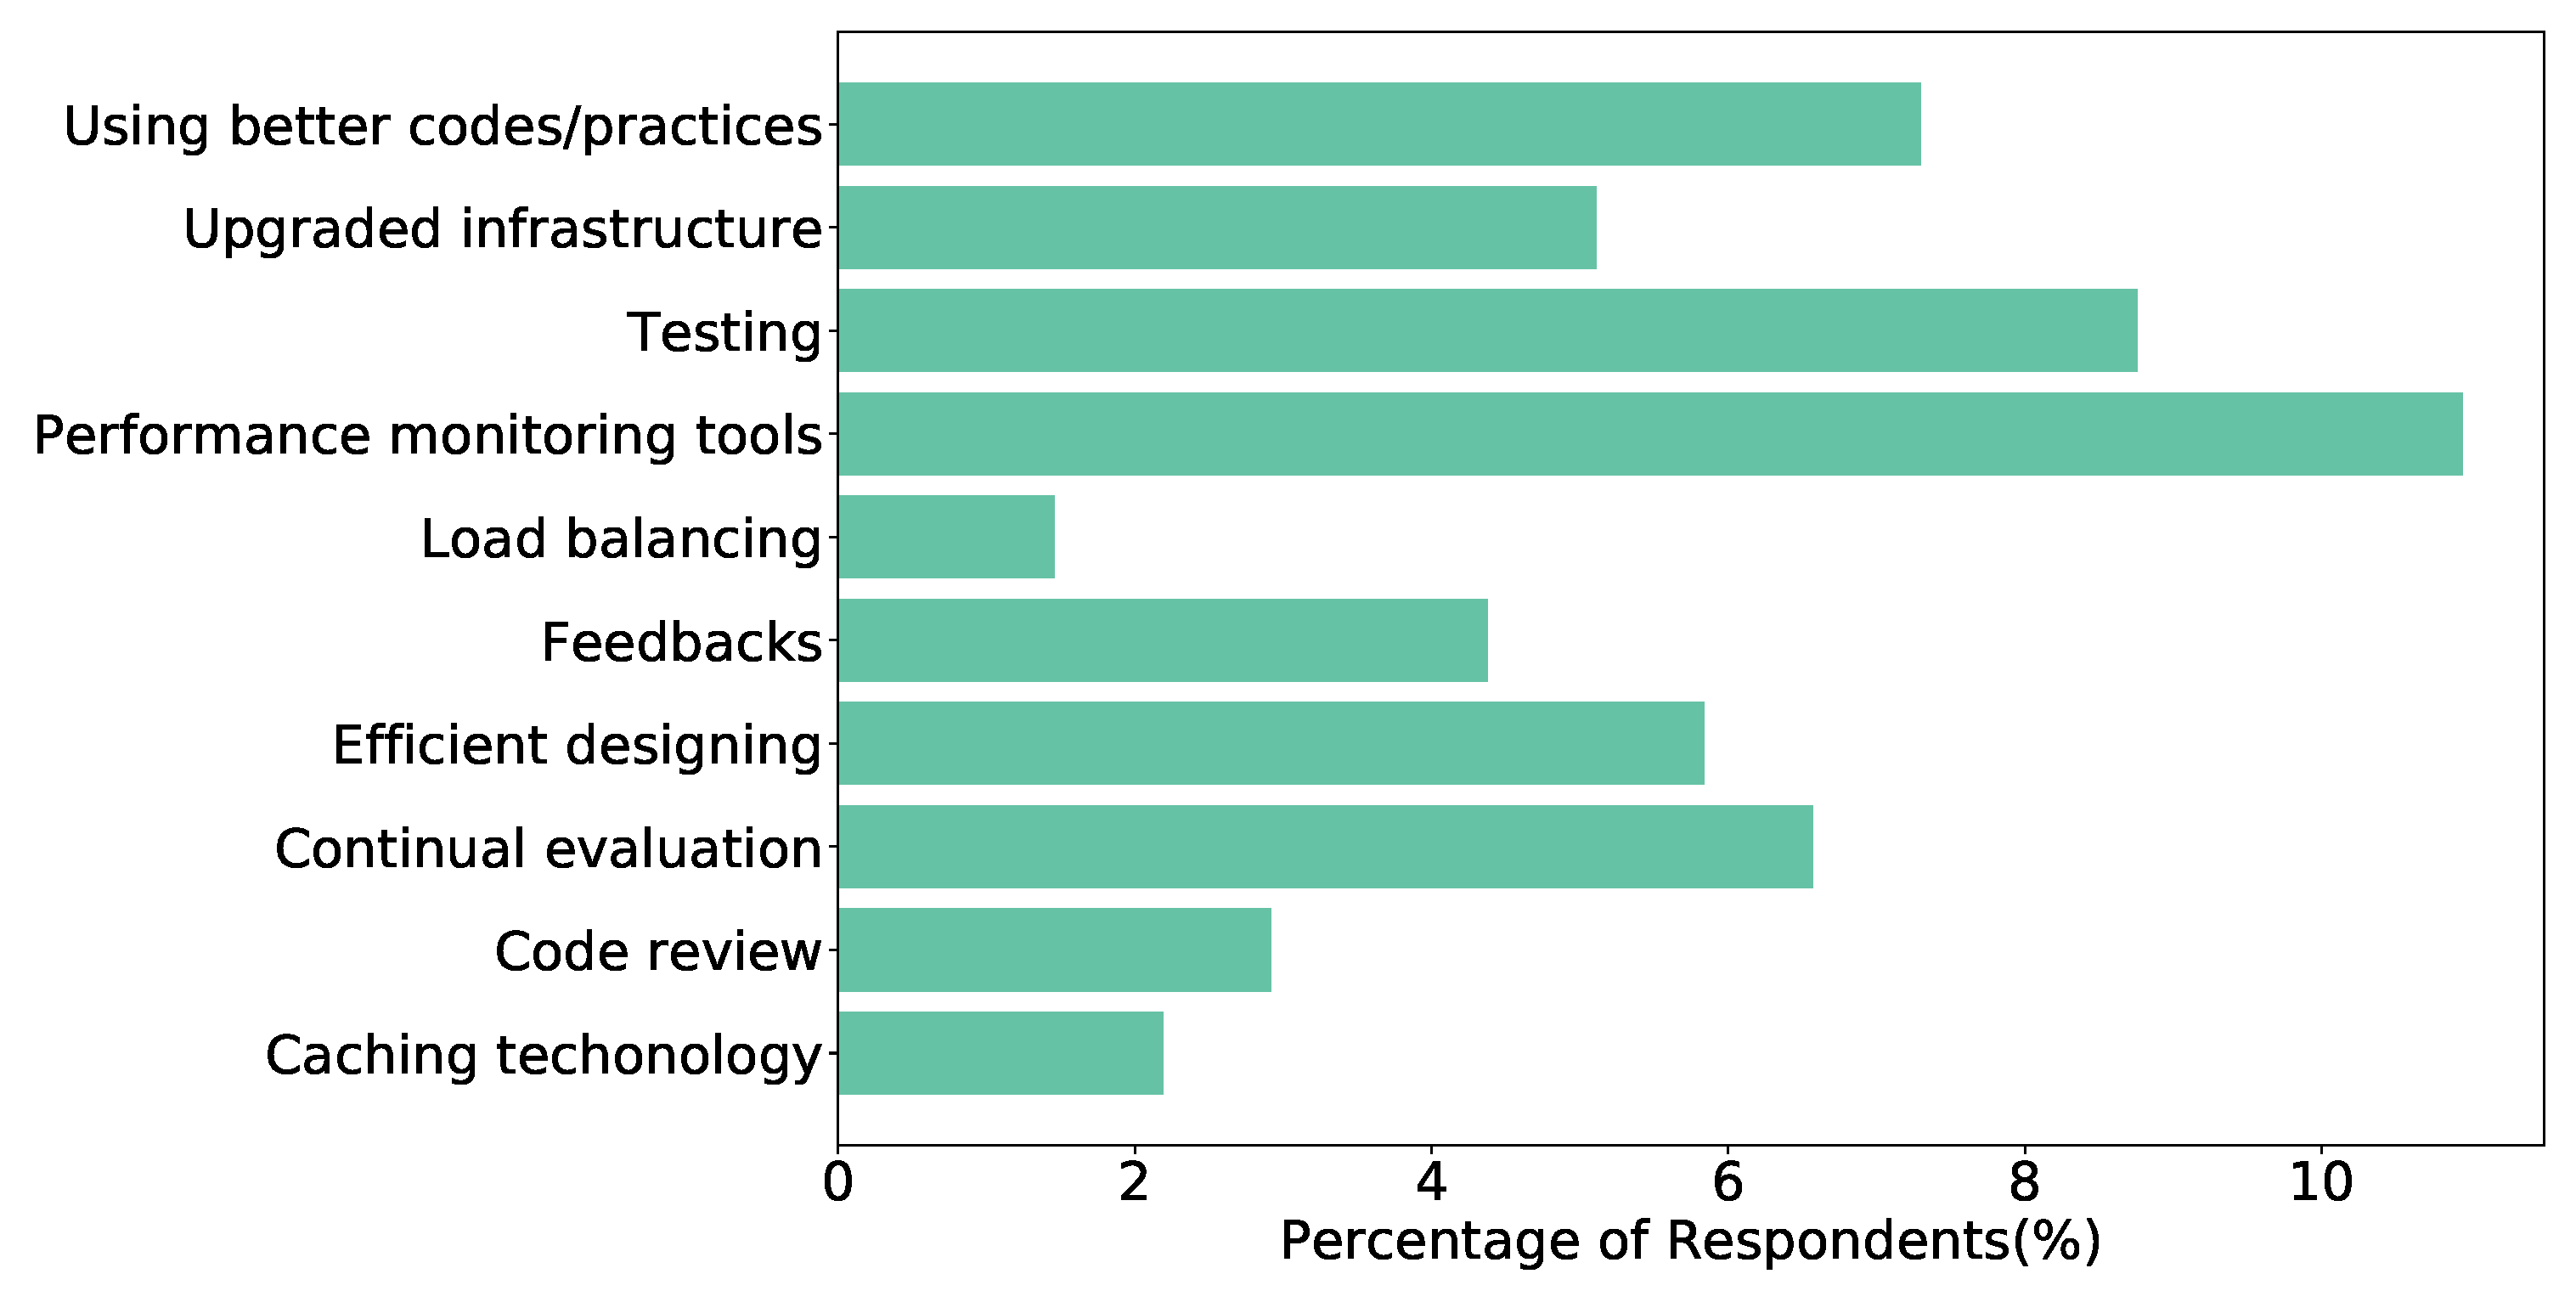
\includegraphics[scale=0.28]{Figures/Performance.eps} 
\caption{Measures to ensure performance of products}
\label{fig:Measures to ensure performance}
\end{figure}
\hfill\\
Software performance indicates how efficient the software is in terms if resource and time. Testing tools such as load testing are common measure\cite{Liu2009} to ensure performance of a software on this regard Bangladesh SE industry follows the same measures. According to our respondents the top three performance ensuring method in Bangladesh SE industry is use of tools, test and better codes/practices or design-implementation level measures. 
\begin{enumerate}

    \item \textbf{Caching Mechanism}: Caching mechanism improves performance by reducing response time. 
    \surveyquote{... Good Caching}{29}
    
    
    \item \textbf{Emphasize on design}: Software performance is dependent on architecture of system. 5.84\% respondents emphasize on design to ensure performance.
    \surveyquote{By careful designing}{24}
    
    
    \item \textbf{Testing}: Performance is ensured by various rigorous testing phase. The phase includes load testing, stress testing, integration testing.
    \surveyquote{By rigorous testing and checking performance testing}{17}
    
    
    \item \textbf{Emphasize on Infrastructure}: 5.11\% respondents use upgraded infrastructure to ensure performance. These infrastructure includes cloud hosting, high end server, new technologies.
    \surveyquote{Amazon Hosting and Quality Software}{85}
    
    
    \item \textbf{Implementing best practices}: Industry standard best practices can improve system performance. 7.3\%respondents ensure performance by implementing best practices. The best practices include compression technology, enforcing design patterns and refactoring.
    \surveyquote{Implementation time carefulness and maintaining a well developed coding standard}{40}
    
    
    \item \textbf{Load Balancing}: Load balancing can improve the system performance by ensuring equal load to all servers. 27.1\% respondents think of using load balancing as a measure to maintain performance.
    \surveyquote{Optimizing number of HTTP requests, Asynchronous programming, Caching, CDN, Load Balancing, nginx, varnish, compression of data, Continuous monitoring, Load testing, stress testing}{42}
    
    \item \textbf{Performance Monitoring Tools}: There are various performance monitoring automated tools from which we can measure the overall as well as component-wise performance of a product. 10.95\% respondents use these tools to measure performance.
    \surveyquote{take help of different performance monitoring tools and dashboard, analyzed data , measure time and memory efficiency of process}{35}
    
    \item \textbf{User Feedback}: It is a great source of performance measure. Taking a time to time feedback from the clients help a company to realise how their products are performing actually. Many (4.38\%) respondents have highly recommended it.
    \surveyquote{Continuous feedback from clients and QA team}{65}
    
    \item \textbf{Continual Evaluation}: If there are some problems about performance, it can easily be identified in continuous monitoring and evaluation of the products. 6.57\% of the total respondents have thought of this as a better solution.
    \surveyquote{regular rechecking/running of automation scripts as a automation tester}{14}
    
    \item \textbf{Code Review}: About 2.92\% people have said that a proper and attentive code review can reduce the faults in the codes and therefore enhance the performance of a software.
    \surveyquote{The code quality is assessed by the different team members during code review, followed by designing new ways to solve issues in the product that are time-intensive.}{15}
\end{enumerate}

\subsubsection{Scalability}
\label{Scalability}
\begin{figure}[htbp]
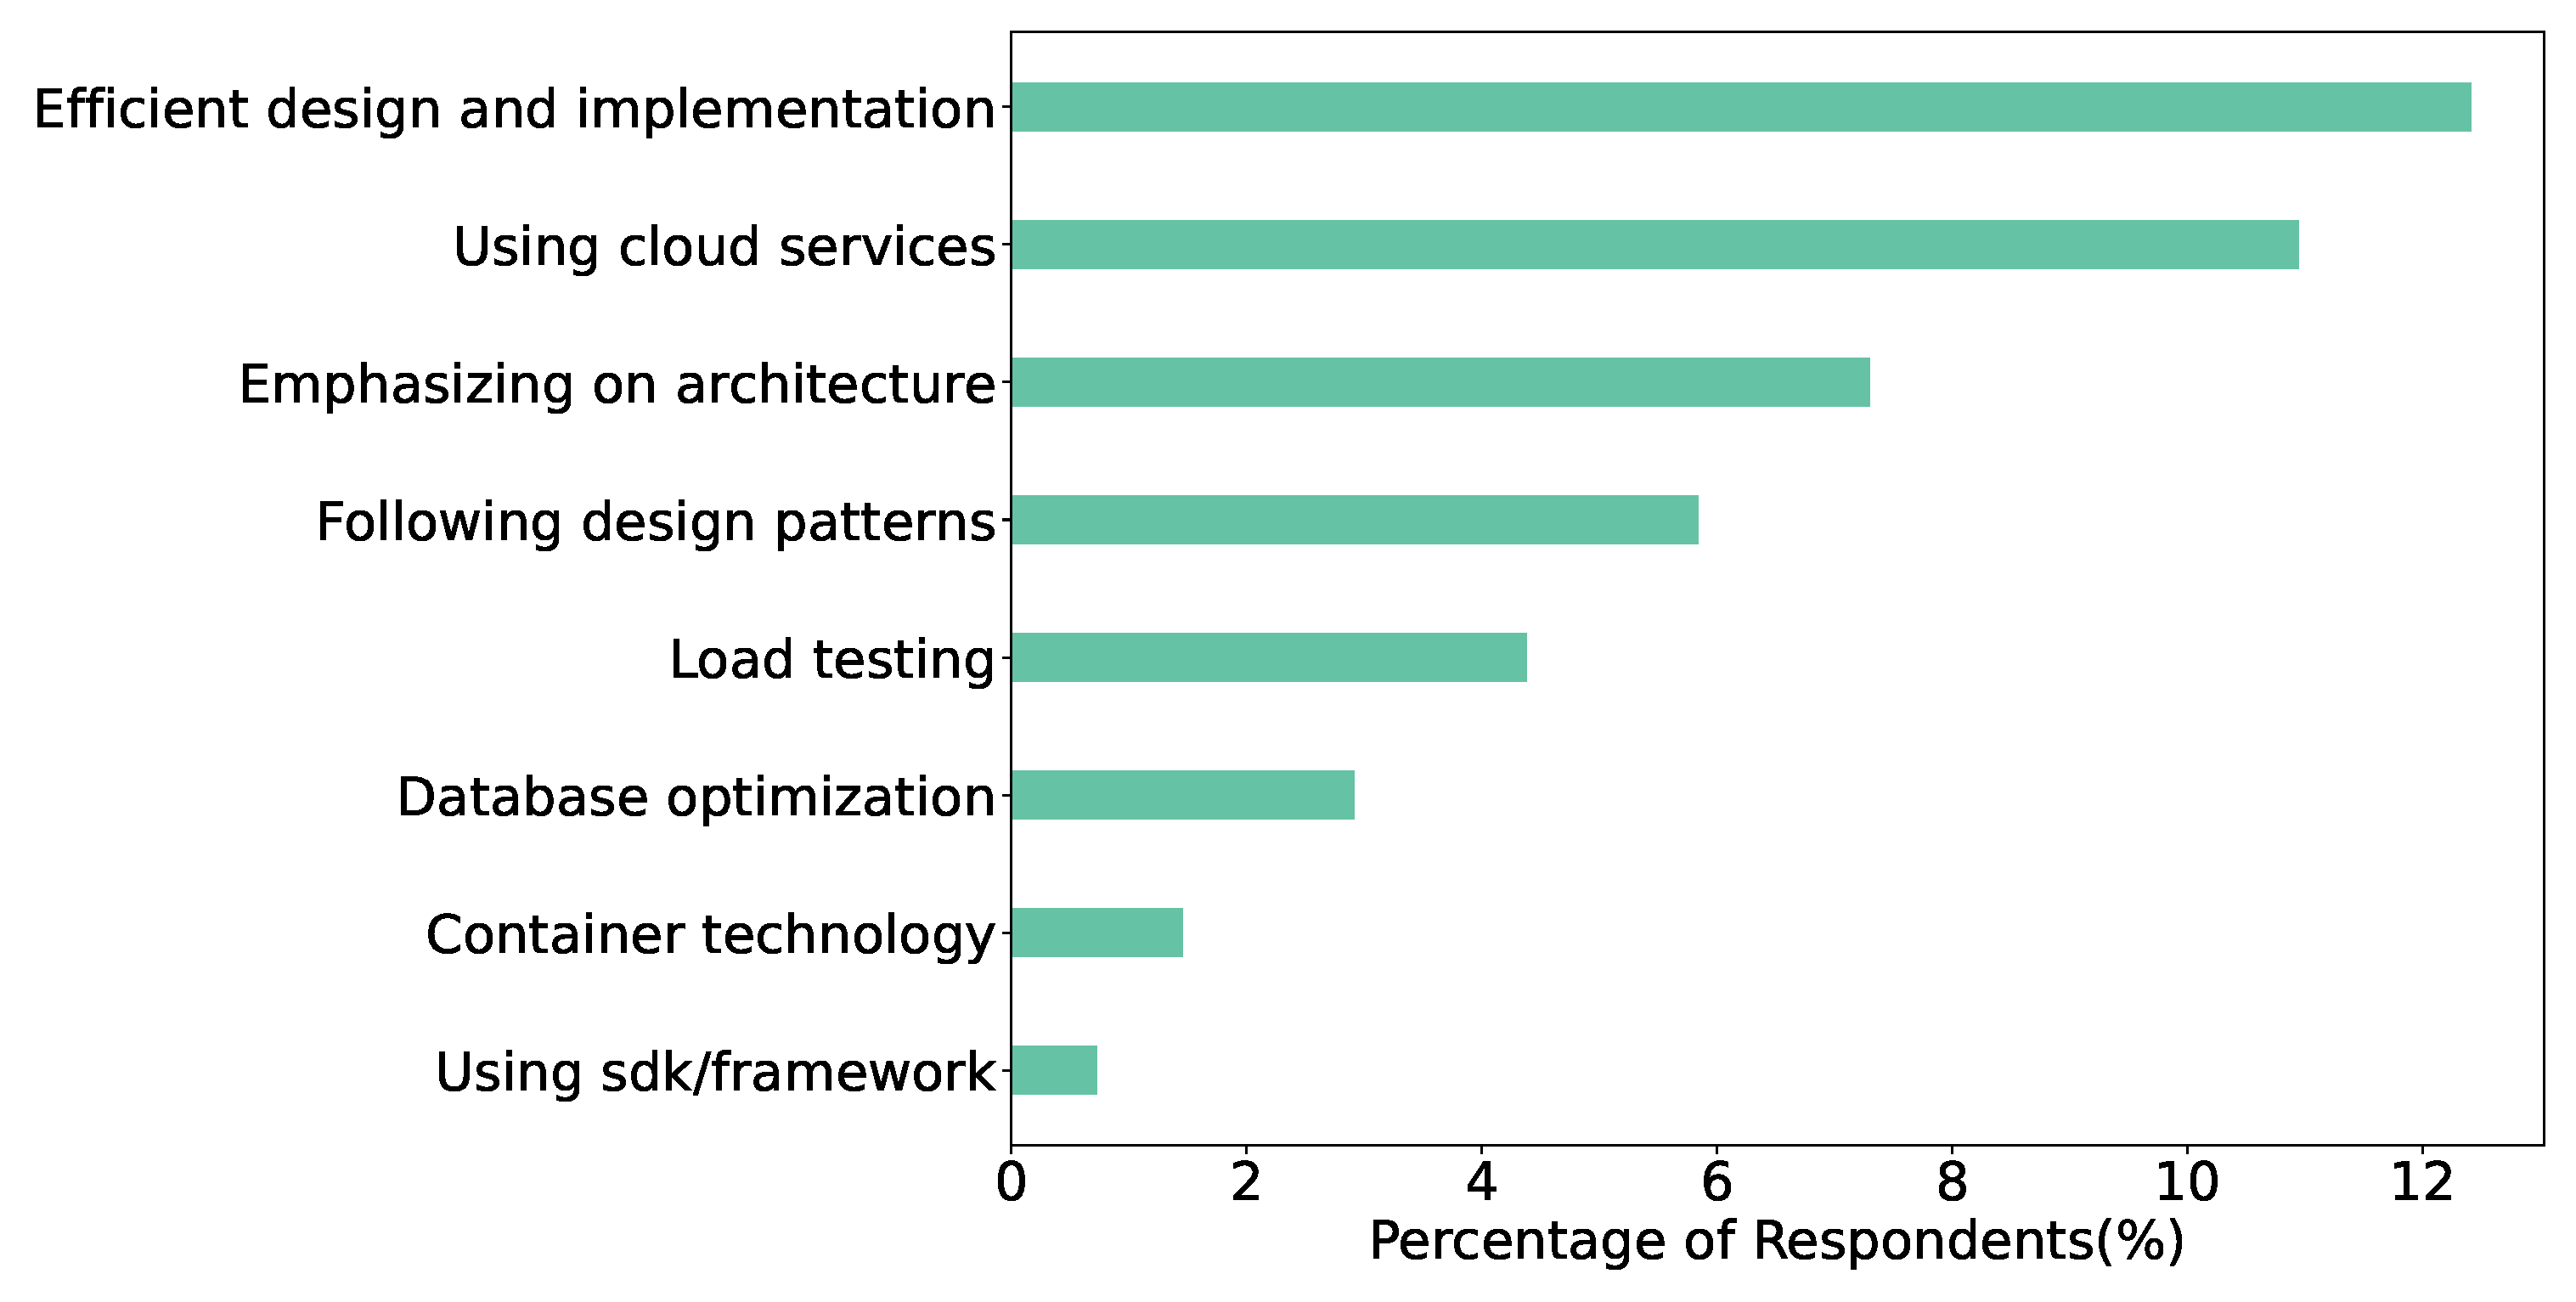
\includegraphics[scale=0.28]{Figures/Scalability.eps} 
\caption{Measures to ensure scalability of products}
\label{fig:Measures to ensure scalability}
\end{figure}
\hfill\\
 Software scalability defines the ability to scale up a solution. Issues with little importance can impede scaling up. Thus proper measures should be taken from design stage to ensure the scalability of system. Recent days the cloud services offer tools to accomodate custom reactive scaling strategies. Thus, it has become easier to ensure scalability using cloud services \cite{Falatah2014}. Our results  also follows the world trend, usage of cloud services has placed 2\textsuperscript{nd} in terms popularity of scalability measures in SE industry of Bangladesh.
\begin{enumerate}
    
    \item \textbf{Following Certain Design Patterns}: There are some design patterns which inherently help us in time of scaling. 5.84\% people think that Following these design patterns will be of great use.
    \surveyquote{Following certain design patterns}{8}
    
    \item \textbf{Based on Framework}: Modern frameworks ensures scalability by default. 0.73\% respondents solely depends on framework for scalability.
    \surveyquote{following flexible framework which allows better scalability}{14}
    
    
    \item \textbf{Container Technology}: Container technologies includes docker, Kubernetes which ensures OS level virtualization. By standardizing the system, container technologies eases the scaling of an infrastructure.
    \surveyquote{We used Docker technology}{85}
    
    \item \textbf{Database Optimization}: Database optimization includes sharding, clustering, indexing and scaling. 10.3\% respondents optimize database to scale their system.
    \surveyquote{Besides scaling horizontally, database scaling is performed by partitioning tables, along with multi-threaded implementations}{85}
    
    \item \textbf{Efficient Design and Implementation}: 12.41\% respondents emphasizes on  the design and implementation of a scalable architecture.
    \surveyquote{During implementation we always keep in mind about the scaling factor}{40}
    
    \item \textbf{Emphasizing on architecture}: 7.3\% respondents emphasized on architecture. It is mostly micro-service architecture which they use to ensure scalability.
    \surveyquote{We follow the micro-service architecture. In a nutshell, we scale up the module vertically which is necessary. We use docker along with Jenkins for automatic deployments and scaling.}{10}
    
    \item \textbf{Load Testing}: Load testing can be used to check the scalability of a system. 4.38\% respondents use load test to check wheather their system is scalable or not.
    \surveyquote{through load testing and load simulation.}{35}
    
    \item \textbf{Using Cloud Services}: 10.95\% user depends on Clod services like AWS and Azure  for the scalability of system. Modern features like elastic load balancing and  auto- scaling makes it easy to ensure scalability.
    \surveyquote{Using AWS Elastic Load Balancer}{28}
    
    
    
\end{enumerate}

\subsection{RQ5:What are the personal expectations and desire reigning in the industry?}
\label{RQ5}
This is the most interesting question. In fact, this question truly answers about the existing condition of our software industry. There are many problems and every one of them has solution. All about these have come into this question beautifully. Every employee has something to tell to their managers. Likewise, every manager has some demands from his subordinates. Not only these, they all have some expectations from government and also universities. All of these expectations are included in the answer of this research question.

\begin{itemize}
    \item Expectation from Managers
    \item Expectation from Employees
    \item Expectation from Potential Candidates
    \item Expectation from Universities
    \item Expectation from Government
    \item Training provide by Companies
\end{itemize}


\subsubsection{Expectation from Managers}
\label{Expectation from Managers}
\begin{figure}[htbp]
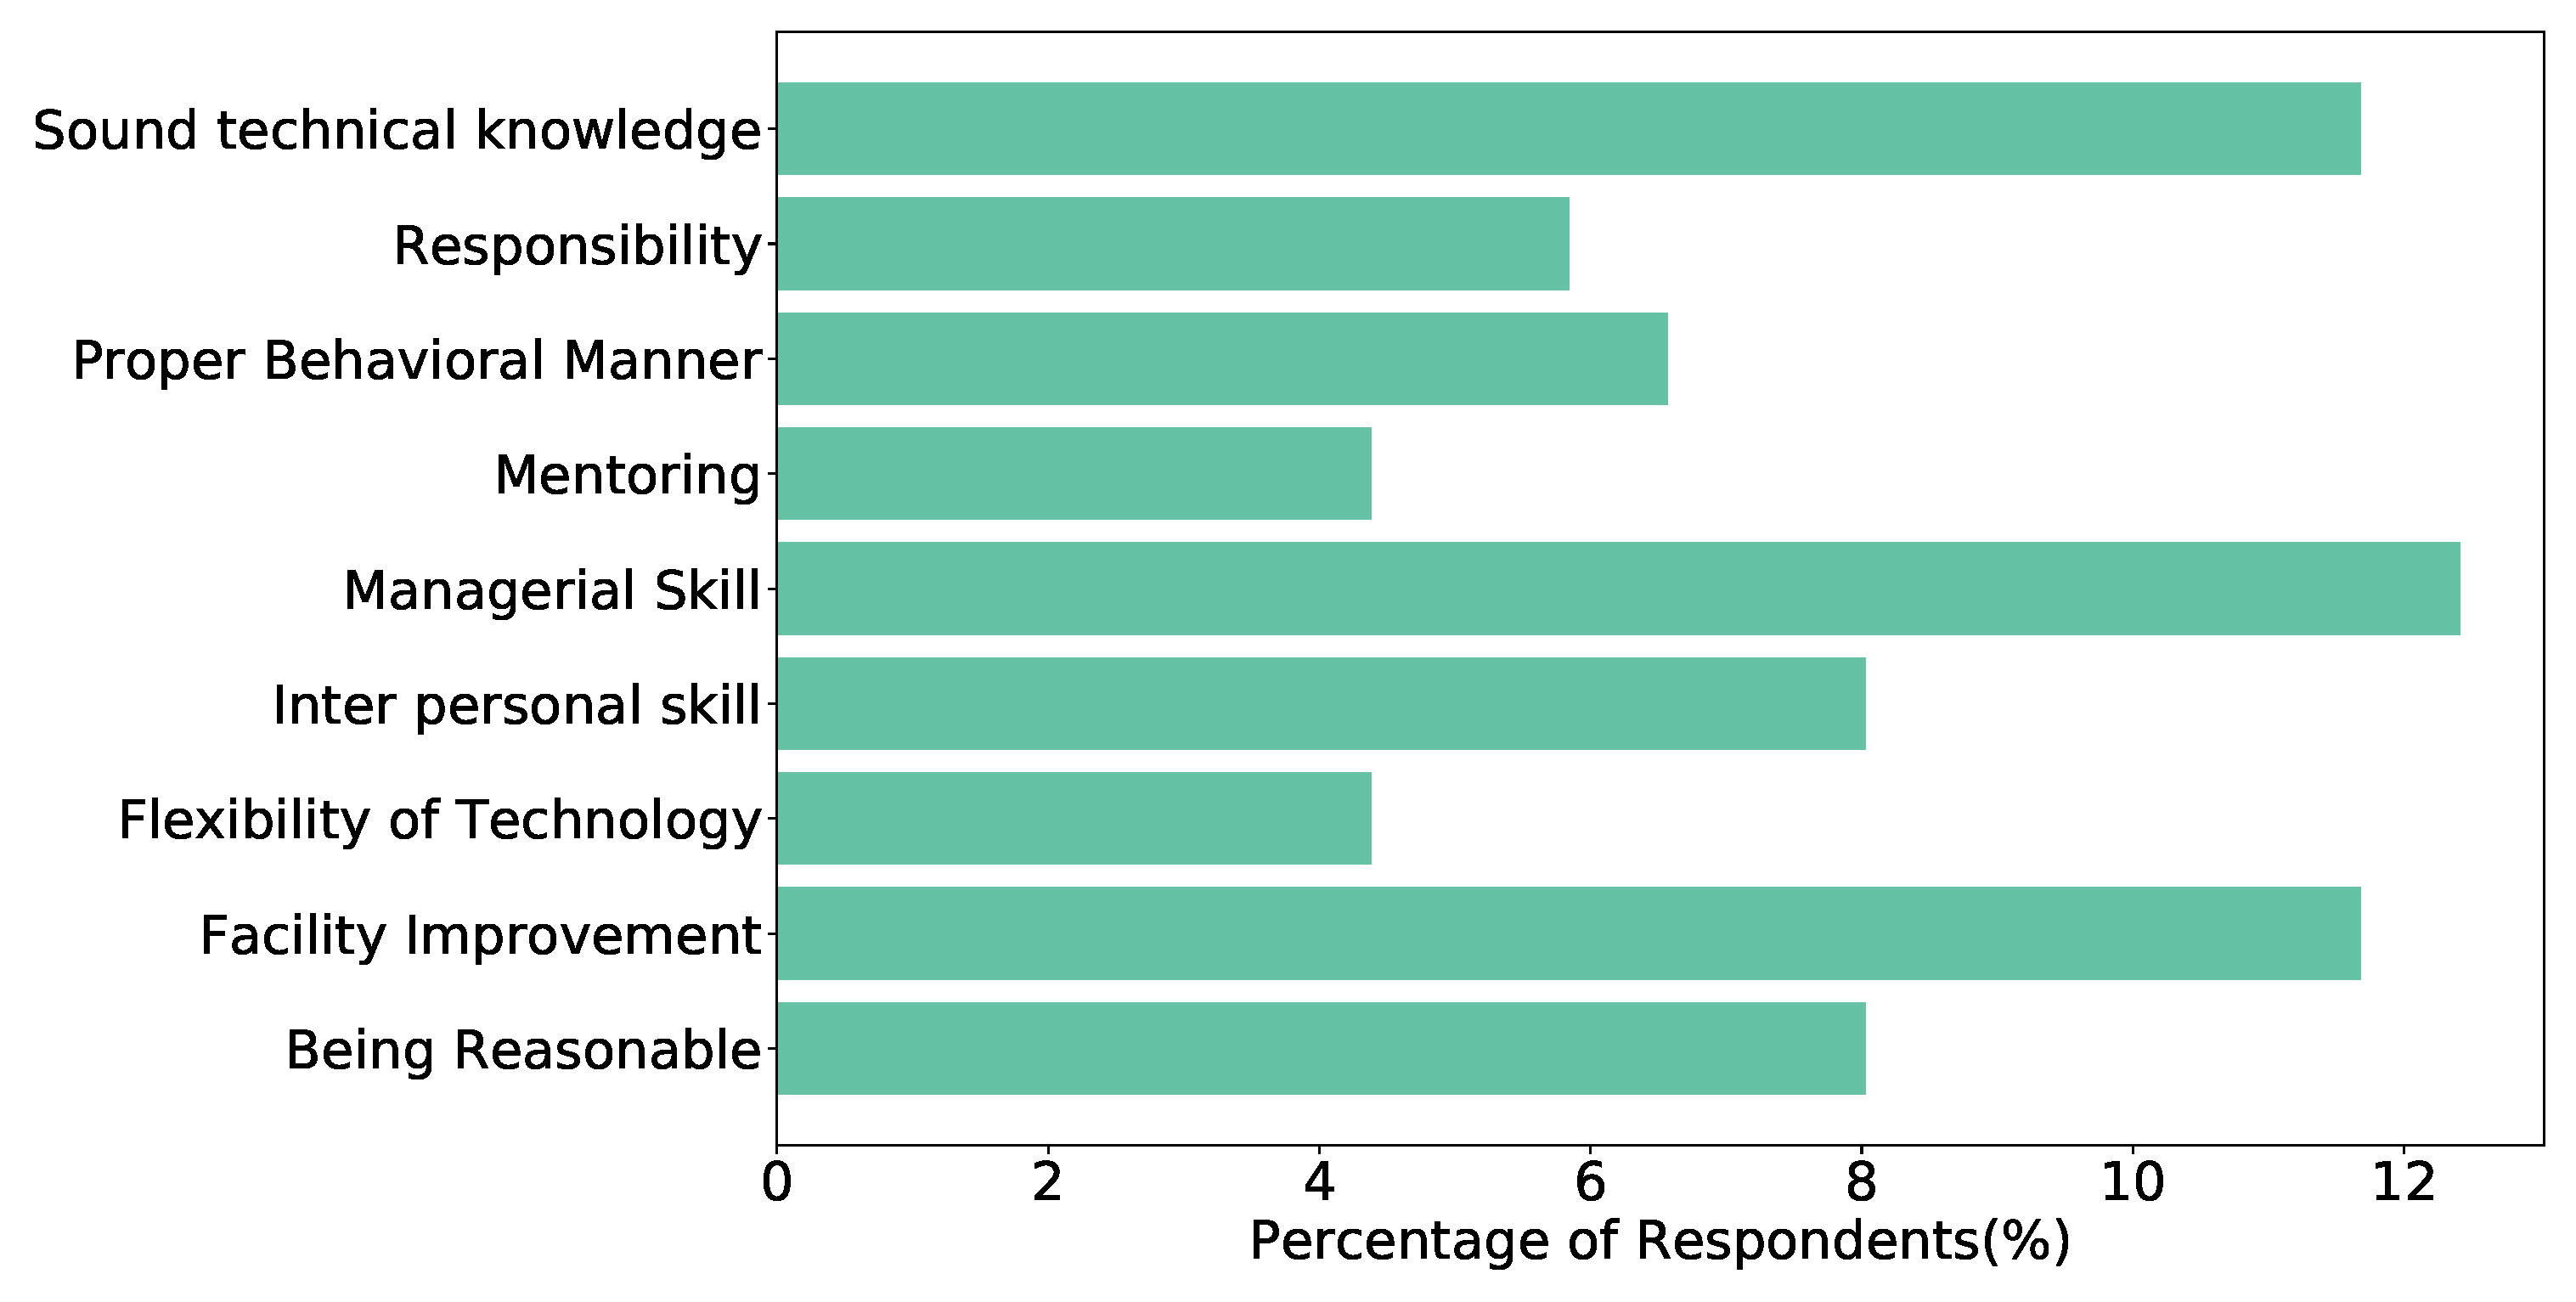
\includegraphics[scale=0.28]{Figures/Managers_Expectation.eps} 
\caption{Respondents expectation from managers}
\label{fig:managers expectation}
\end{figure}

\begin{enumerate}
    \item \textbf{Proper behavioural manner}: 6.57\% respondents expect well behaviour from management. It is clear from survey responses employees hates micro-management the most.
     \surveyquote{Well Behaved and Proper Project Timeline}{28}
    
    
    \item \textbf{Being Reasonable}:  The managers should be reasonable in decision making. In order to get acquainted with the needs and necessities of the employees, managers should have a wide open view towards their desire. About 8.03\% of the respondents have expressed in this way.
    \surveyquote{Give reasonable time for a task and do proper comment on that task}{38}
    
    
    \item \textbf{Flexibility of Technology}: It is very important for the managers to be up-to-date with the latest technology. Managers without a strong background of technical knowledge are really difficult to work with. 4.38\% of total respondents have demanded for a manager with sufficient technical knowledge. 
    \surveyquote{Allow to use latest technologies and good practice to ensure company and their employee are updated with the current world. And also honor according to knowledge and quality works. In the company should have knowledge sharing, training sessions}{48}
    
    
    
    \item \textbf{Responsibility}: Managers should take the responsibility for the works being done. A responsible manager can inspire the employees under him to a great extent. About 5.84\% of the total respondents aspire for a responsible manager to work with.
    \surveyquote{Take responsibility}{82}
    
    
    \item\textbf{Facility Improvement}: 11.68\% respondents mentioned that they look for facility improvements from managers. These facilities include increased remuneration, good working environments, team building events, positive recognition, yearly evaluation etc.
    \surveyquote{Ensuring an environment where positive criticisms regarding code and people can be done.}{57}
    
    
    \item\textbf{Inter Personal Skill}: 8.03\% respondents expects inter personal skills among managers. The skills include proactive, leadership attitude, good communication skill and empathy.
    \surveyquote{Ownership, Proactiveness, Leadership attitude, Good inter-personal and communication skills}{42}
    
    
    \item\textbf{Managerial Skill}: The managers should have solid technical knowledge. He/she must be farsighted. One of the most important part of this post is management of requirements. He should have clear  understanding of required manpower and resources. Respondents marked that timeline management is another managerial skill they expect from managers.
    \surveyquote{1. Strong grasp on the requirements before assigning me to a project 2. Maintain informed and feasible deadlines}{8}
    
    
    \item \textbf{Mentoring}: Respondents also look  a mentor character in manager. They expect direction, advice and opportunity from managers for their career growth.
    \surveyquote{To supervise and to advise to follow specific career plan}{9}
    
    
    \item\textbf{Sound Technical Knowledge}: 11.68\% respondents emphasizes on technical knowledge among managers.
    \surveyquote{Should be technically active}{14}

\end{enumerate}


\subsubsection{Expectation from Employees}
\label{Expectation from Employees}
\begin{figure}[htbp]
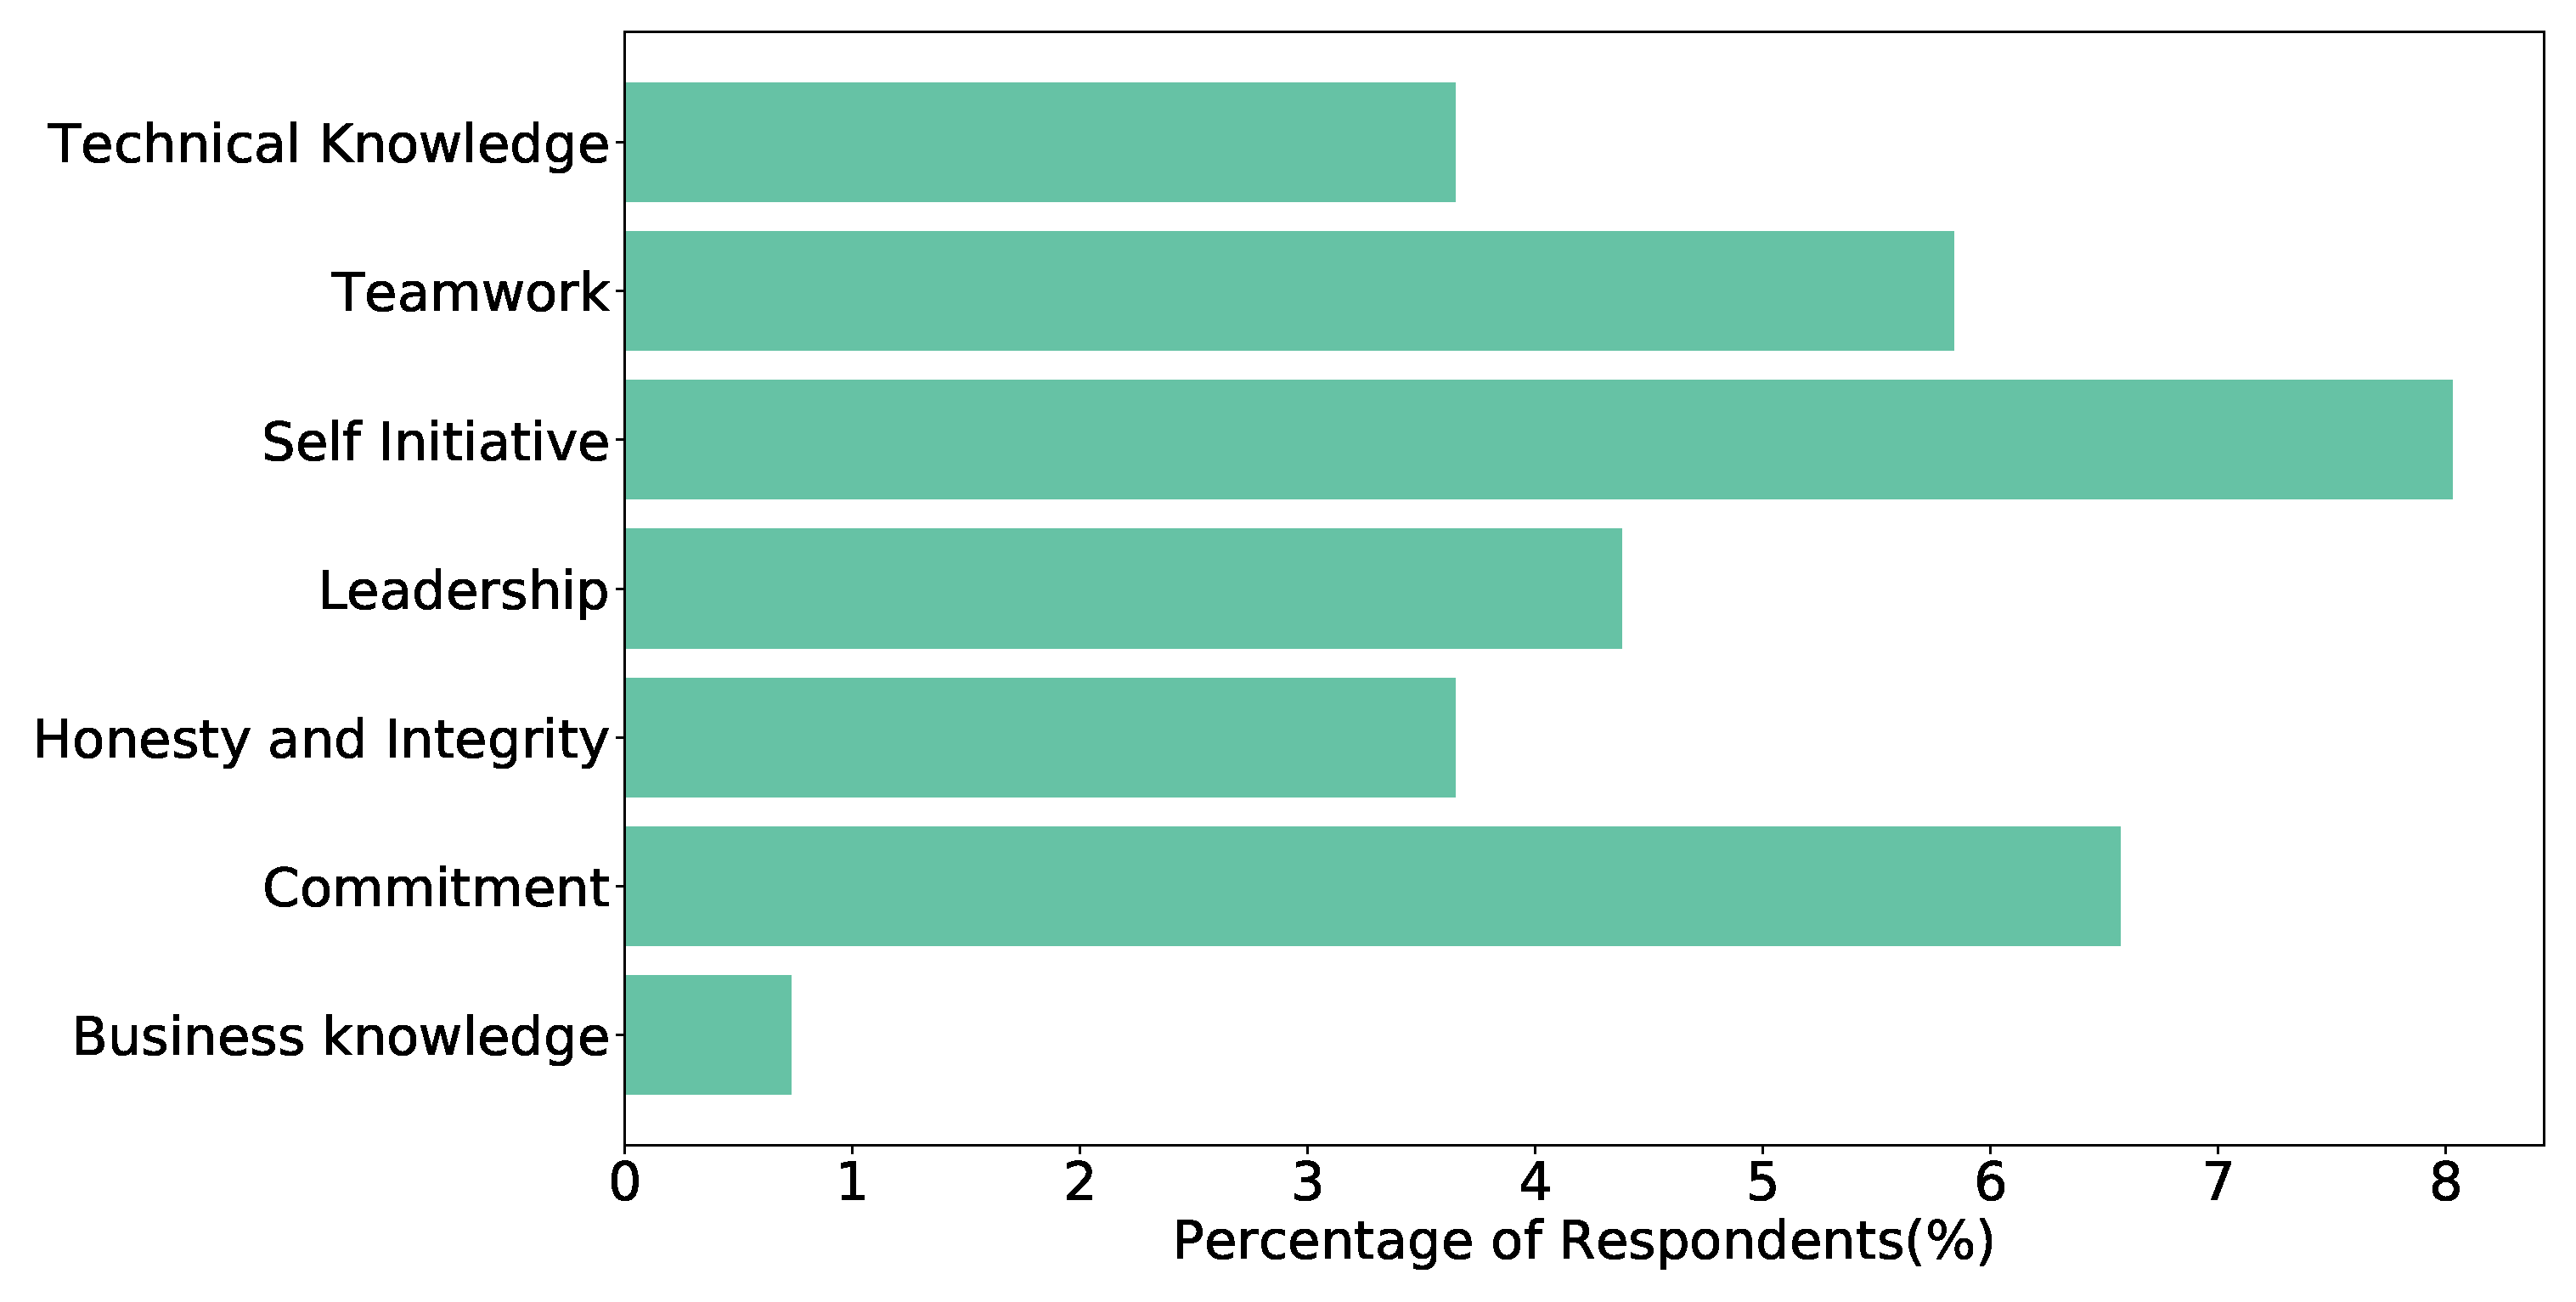
\includegraphics[scale=0.28]{Figures/EmployeeExpectation.eps} 
\caption{Respondents expectation from employees}
\label{fig:employees expectation}
\end{figure}

\begin{enumerate}

    \item \textbf{Technical Knowledge}: 3.65\% respondents look for solid technical knowledge and clean codes from employees.
    \surveyquote{Code in a way that is a delight to read}{49}
    
    
    
    \item \textbf{Teamwork}:It is very obvious to be expected. In a software industry, not a single product is created single-handedly. A bunch of people from various sectors work on the product, and to make a good product, team work between these members is very important. 5.84\% of the managers responded desired this behaviour from the employees.
    \surveyquote{Employees should be cooperative and share knowledge with each other and work together like family member}{51}
    
    
    \item \textbf{Self Initiative}: An employee should learn in his own interest. In industry, everyone is occupied with himself. There is no space to be spoon-fed. A self-initiative worker will find his way even if there are many obstacles.8.03\% people have appraised self-initiative attitude.
    \surveyquote{Clean code which creates less error. Coming up with optimization proposals on features developed earlier. Documentation in a timely manner}{10}


    \item \textbf{Leadership}: 4.38\% respondents look for leadership attitude like ownership of work, proactive and adaptiveness among employees.
    \surveyquote{Sincere, Feel owner ship of project/product and good teamplayer}{107}
    
    \item \textbf{Honesty and Integrity}: Not only coding and academic knowledge, but also behavioural manner plays a great role in deciding about a employee’s career. 3.65\% people want a well behaved and mannered employee to work with.
    \surveyquote{honesty, integrity, self initiative and clear communication}{35}
    
    
    \item \textbf{Commitment}: 6.57\% managers have demanded commitment from their employees. A more committed employee will give better performance than a less committed employee, as he does not give full attention to the job.
    \surveyquote{They will stay for long term and perform up to expectations, learn from mistakes}{114}
    
    
    \item \textbf{Business Knowledge}:  It is important to have knowledge of business domain when designing a solution or dealing with a customer. Thus respondents look for business knowledge like negotiation among employees.
    \surveyquote{Understanding the business, end user and user stories}{82}


\end{enumerate}


\subsubsection{Expectation from Potential Candidates}
\label{Expectation from Potential Candidates}
\begin{figure}[htbp]
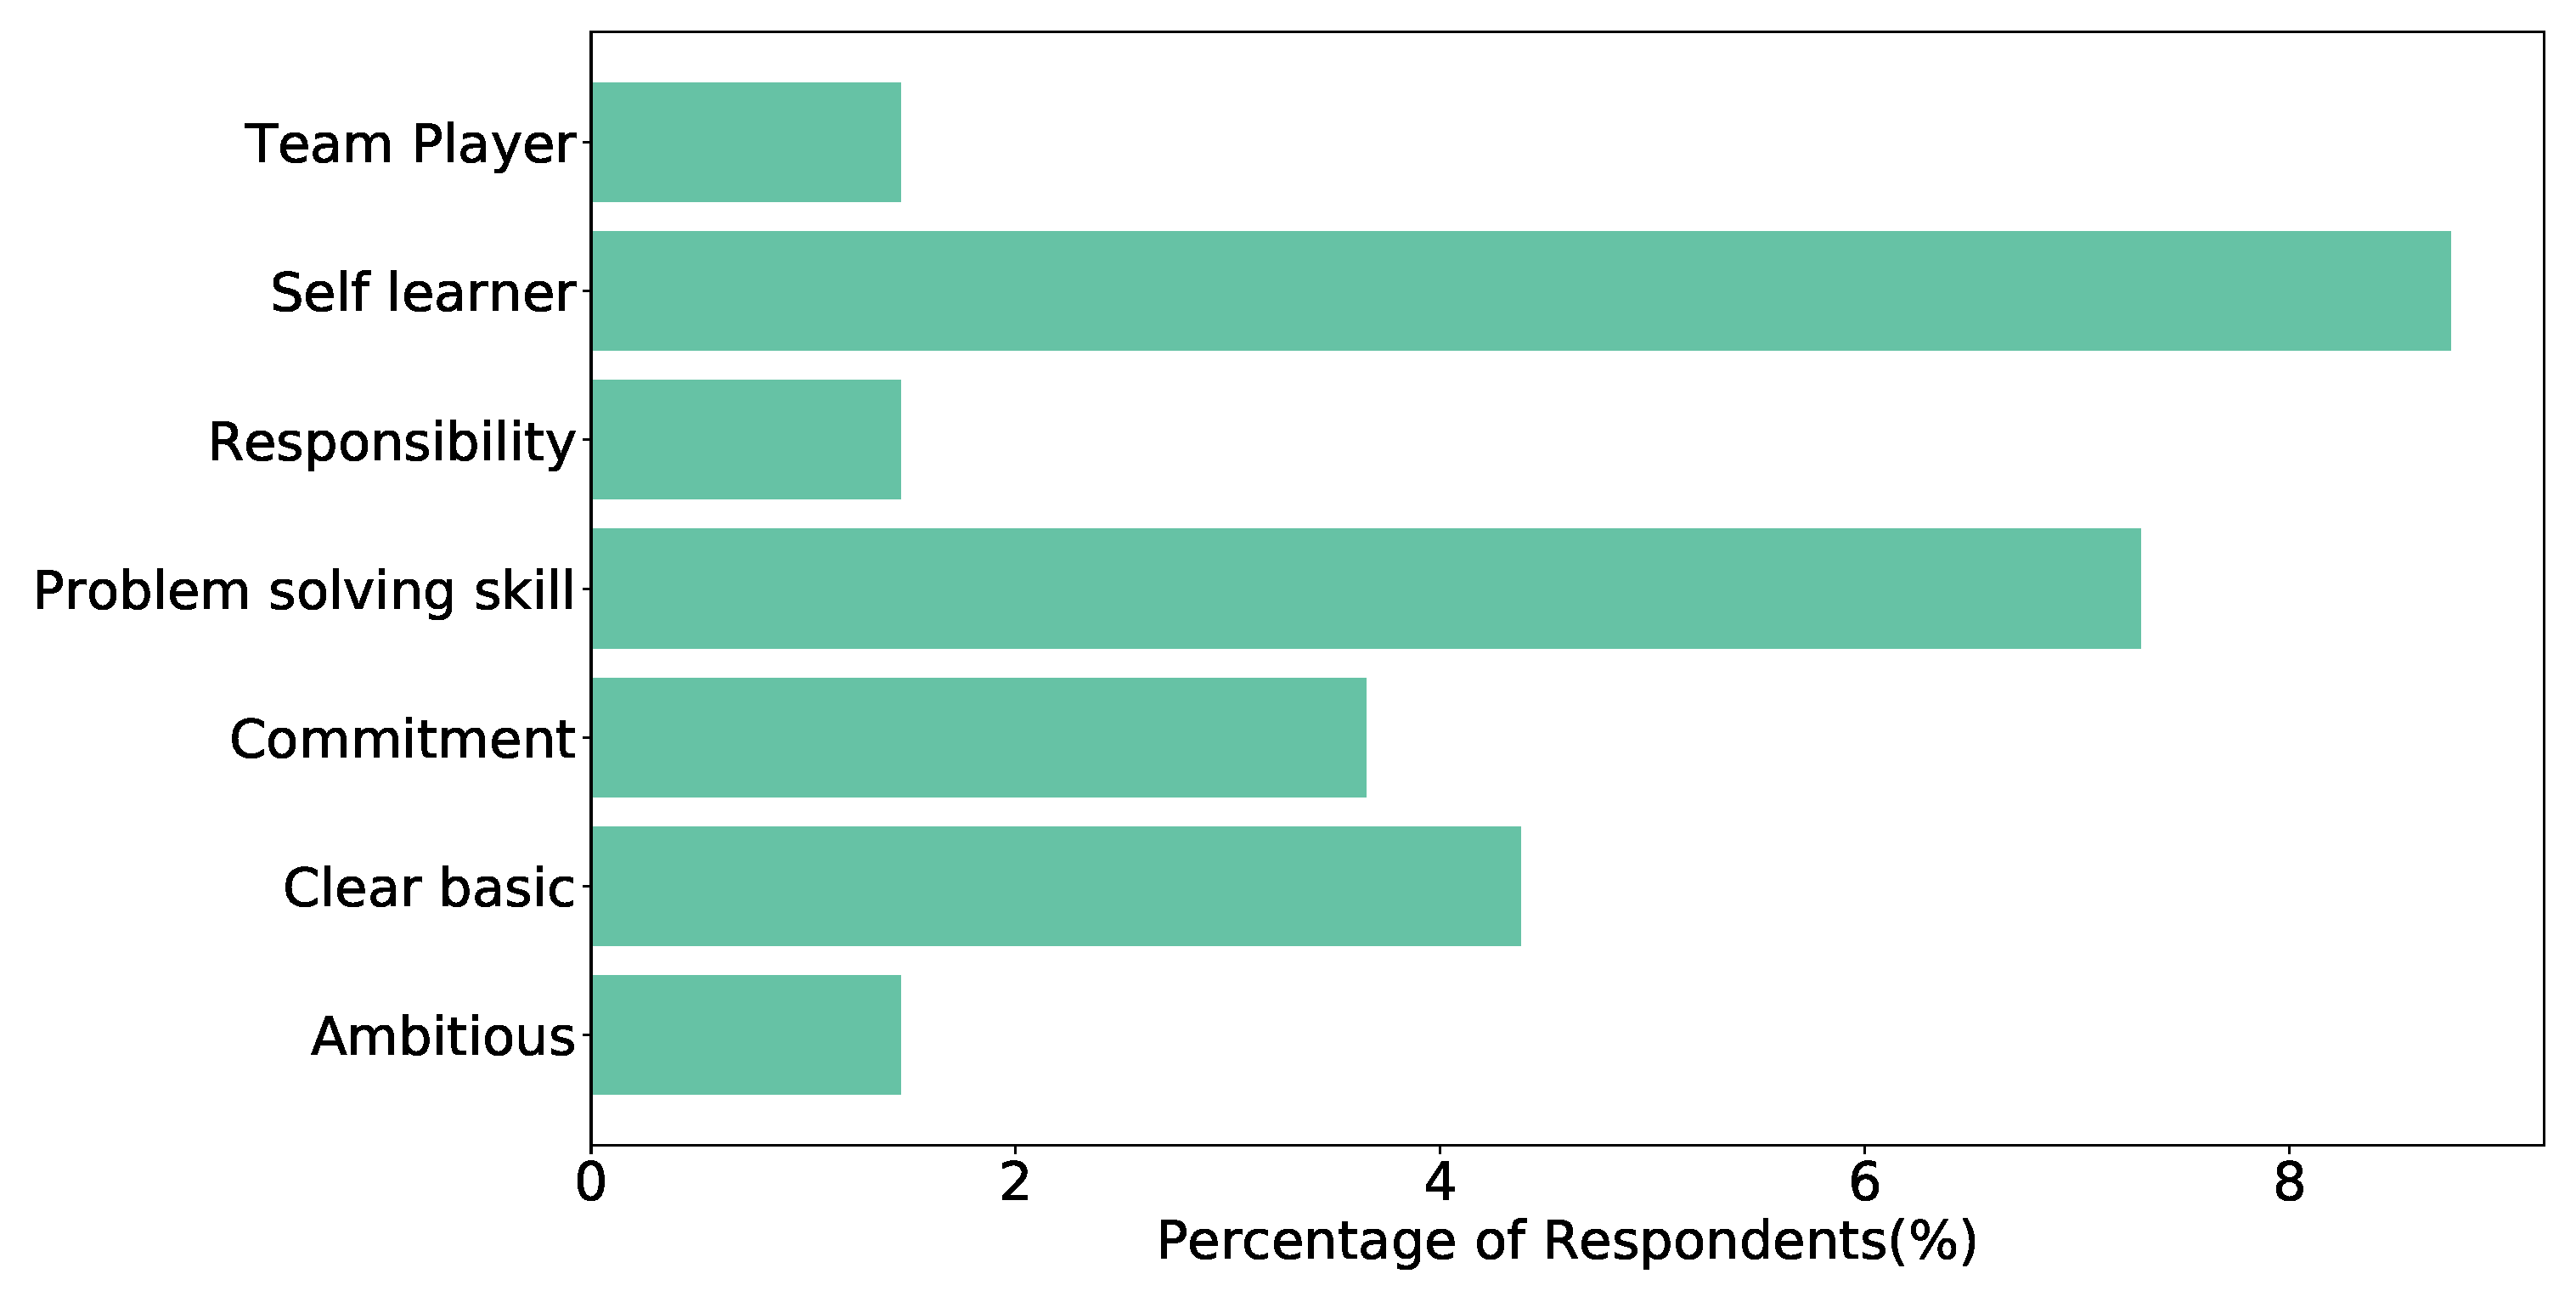
\includegraphics[scale=0.28]{Figures/CandidatesExpectation.eps} 
\caption{Respondents expectation from potential candidates}
\label{fig:candidate expectation}
\end{figure}

\begin{enumerate}
    \item \textbf{Team-player}:Team work plays the most significant role for success in a specific product in any industry. Every potential job candidate should be prepared to work together with a group of people to fulfill the production of a software. 1.46\% wanted to hire a team player than an individual talent.
    \surveyquote{Enthusiastic, Self-learner, Team player}{5}
    
    
    \item\textbf{Self-learner}: Most of the software companies does not have luxury to arrange training or to assign mentor. Thus employers look for self-learning capability among candidates.
    \surveyquote{Self learner, Know well what you know}{53}
    
    \item\textbf{Responsibility}: 1.46\% respondents look for ownership of work or sense of responsibility among potential candidates.
    \surveyquote{taking ownership of responsibility}{66}
    
    
    \item\textbf{Problem-solving Skill}: Problem solving skill distinguishes a potential candidate from others. A candidate with good problem solving capability can adapt to any team. Problem-solving skill is desired by 7.3\% of the total respondents.
    \surveyquote{I am assuming that the potential candidates refer to the freshers in this question. I expect freshers to be very good with problem solving with strong analytical ability. Good university projects are plus}{10}
    
    \item\textbf{Commitment}: 3.65\% of the respondents want commitment from the freshers who are willing to enter into the software industry. He should give his best to attain the goal.
    \surveyquote{Commitment and dedication}{114}
    
    \item \textbf{Clear basic}: Every company want that freshers will have a clear understanding about the basic knowledge. They do not want knowledge about industry, they want clear knowledge about things like programming language, data structures and algorithm. 4.38\% of the respondents want clear basics form the candidates.
    \surveyquote{Professionalism and clear understanding of technologies what they know}{85}
    
    \item\textbf{Ambitious}: 1.46\% respondents prefer ambitious candidates. They look for enthusiasm and hunger for success among candidates.
    \surveyquote{ Knowing what he/she knows and what not, honesty, good problem solving capacities, team-man, absolutely no ego or arrogance, can get things done, ambitious, sincerity, discipline}{42}
\end{enumerate}


\subsubsection{Expectation from University}

\label{Expectation from University}
\begin{figure}[htbp]
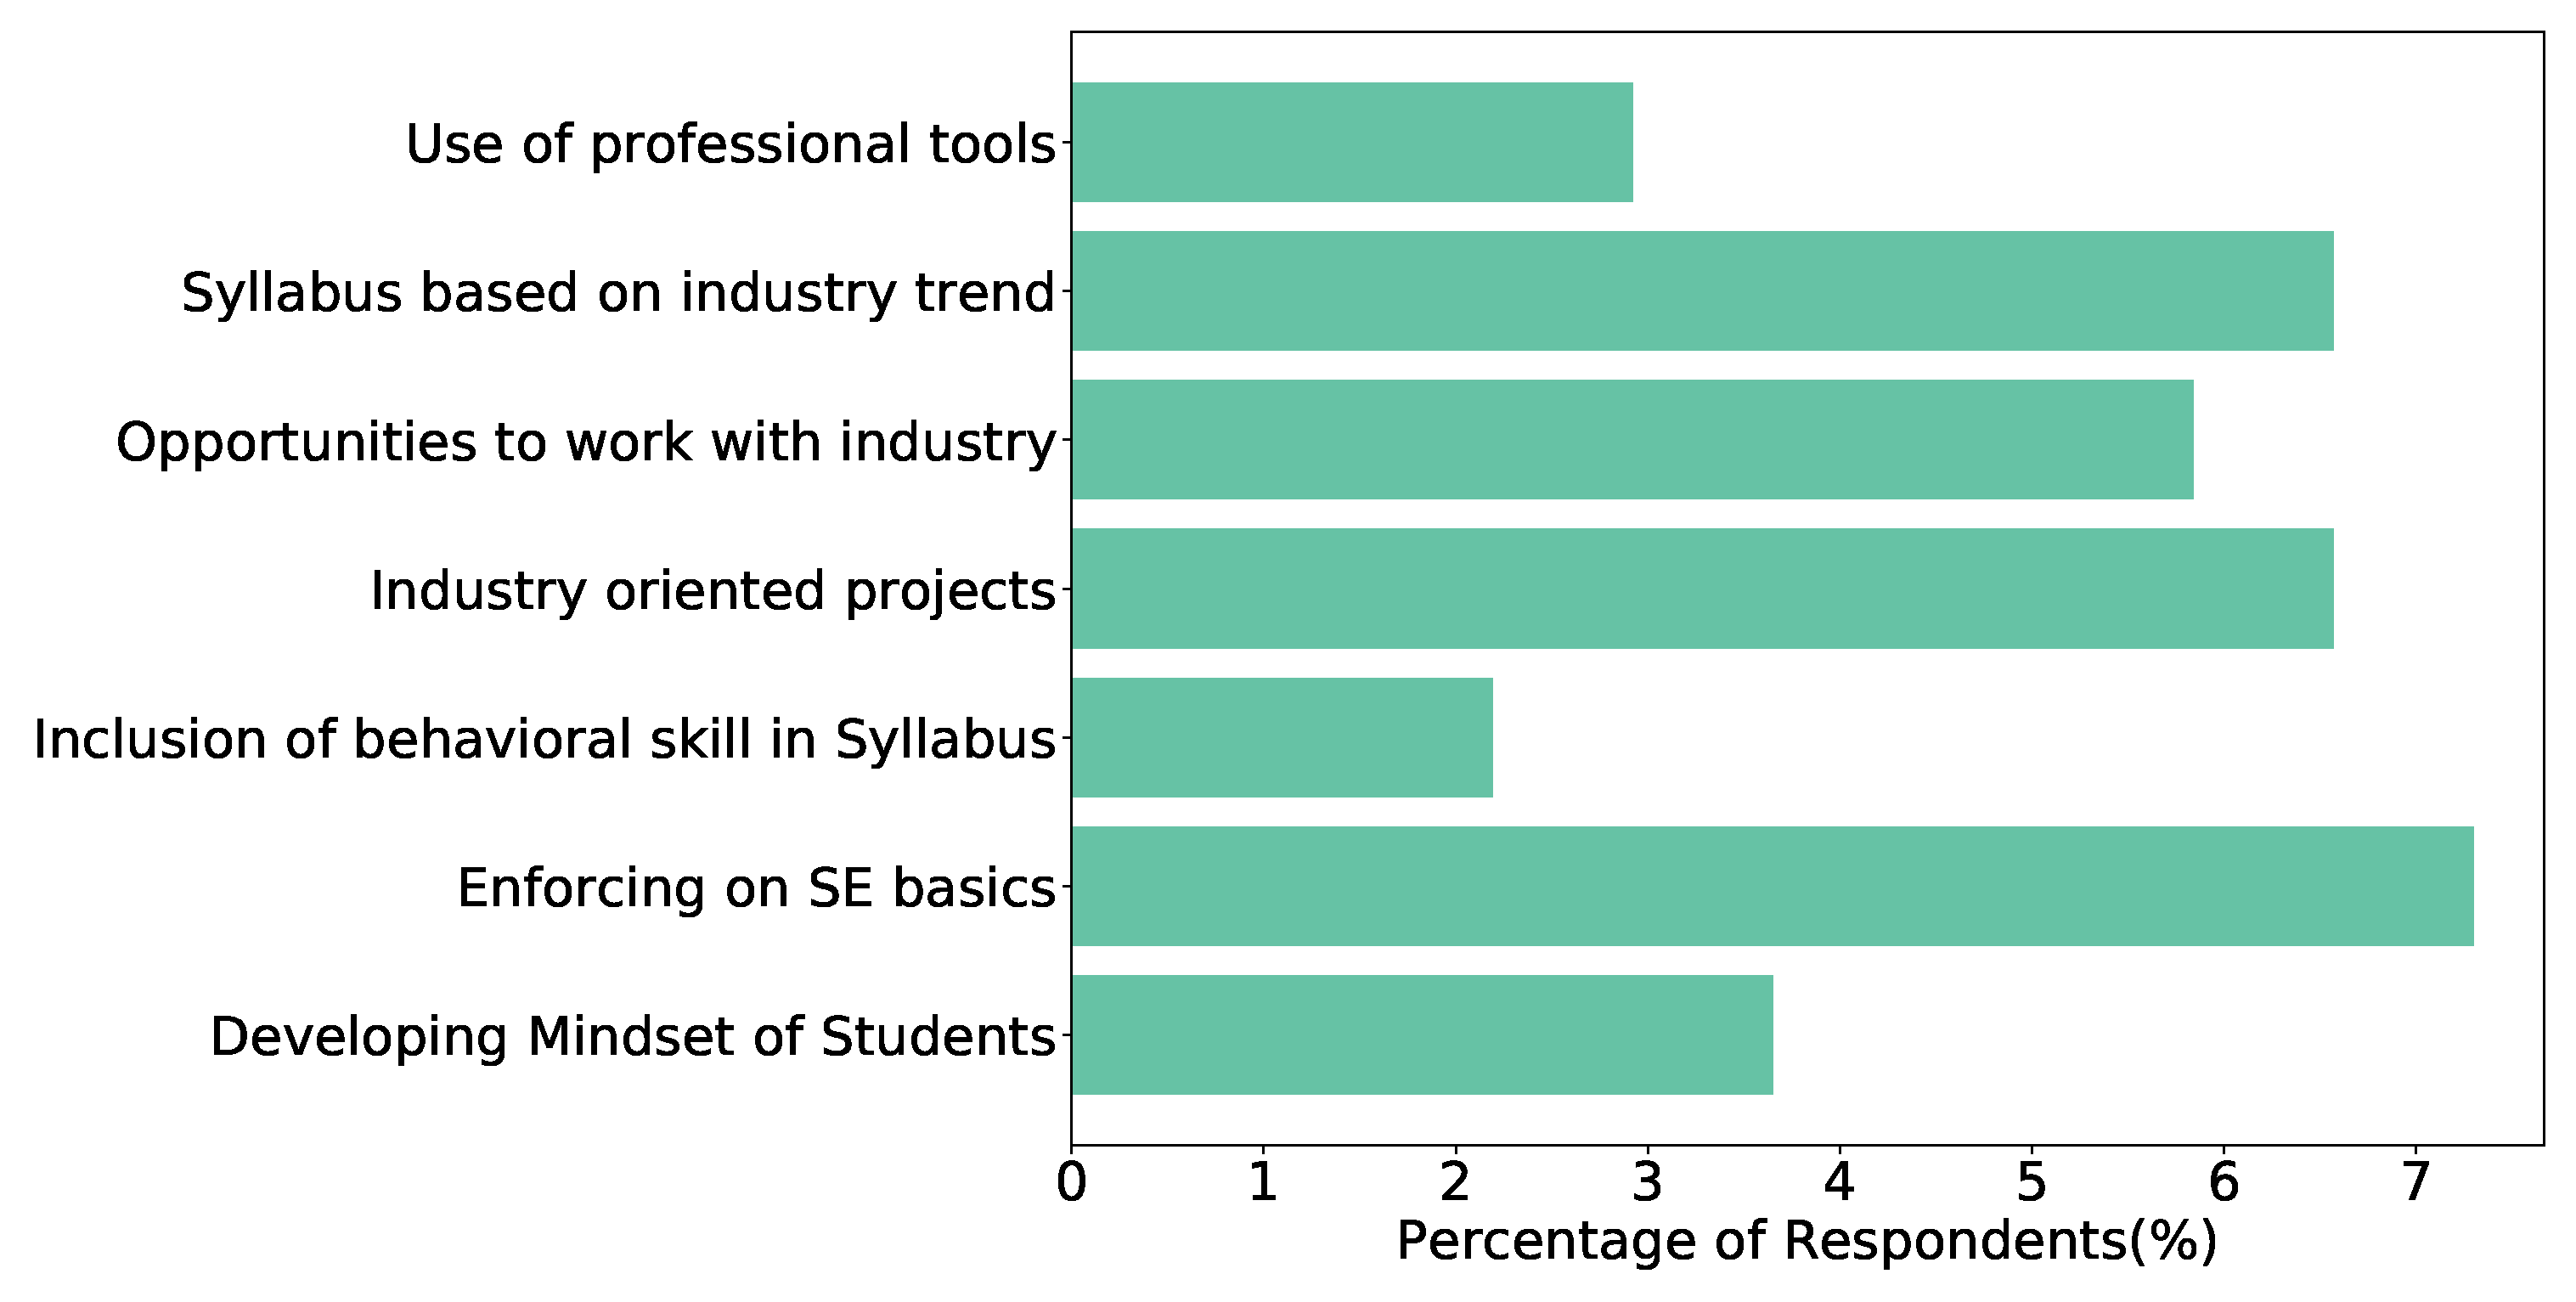
\includegraphics[scale=0.28]{Figures/UniversityExpectation.eps} 
\caption{Respondents expectation from university}
\label{fig:university expectation}
\end{figure}
\hfill\\
To have a vibrant SE industry and to maintain a steady workforce for the industry it is important that universities meet the expectation from the industry. As seen in Figure \ref{fig:university expectation}, industry owners/experts expect emphasis on SE basic and on current trends, they also seek for the opportunity to collaborate with the universities. The result coincides with  a study conducted by Radermacher et al. \cite{Radermacher2013}. According to their study, SE basic (Project Management, Software Tools, Testing) is the second area where graduate students are deficient in knowledge\cite{Radermacher2013}. Though behavioral skill or soft skill enables faster integration and happier teams only 2.19\% respondents emphasize on inclusion of behavioral skill in syllabus, the scenario is quite different in New Zealand. In a survey conducted by Stevens et al.\cite{Stevens2016} it is found that industry experts emphasize on behavioral skills after technical skill. They also found that those skills are un-trainable in work place. Thus it is the duty of university to train graduates with required skill set.
\begin{enumerate}
    
    
    \item \textbf{Inclusion of behavioral skill in Syllabus}: Being a good coder is difficult, but being a good human being is much more difficult. In industry, a person has to meet a large variety of personalities, and only a well behaved individual will find it easy to work with them. About 2.19\% people have implied about it.
    \surveyquote{Teach students Professional Ethics and Practices, Tie-up with Industry Practices and Problems, Solutions or Research Paper for any specific or generic Technical/Administrative problems}{108}
    
    
    
    \item \textbf{Syllabus based on industry trend}:It is seen in some universities in our country that they are teaching on a syllabus which was designed a very very long time ago. Since then software industry has advanced a long way. 6.57\% of our respondents think that these age-old academic curriculum should be changed and new latest topic should be added.
    \surveyquote{Concentrate on applied science with theory. Change syllabus based on current trend each year. Apply internship to relevant organisations}{5}
    
    
    
    \item \textbf{Opportunity to work with industry}:  As many students will be joining the industry after graduation, it will be very convenient for everyone if they are acquainted with the industry in their varsity life. 5.84\% respondents have felt the necessity of industry-academia correlation.
    \surveyquote{Create opportunities to work with industry solving the problems we are facing in the industry. Sometimes we are so busy with developing features that we lack the opportunity to run some researches about our tasks. University projects can be subjected to s...}{10}
    
    
    
    \item \textbf{Industry oriented projects}: 6.57\% respondents wants that in university student should engage in projects which is relevant to industry.
    \surveyquote{Connection with industry, realistic teaching, internship arrangement for students}{59}
    
    
    
    \item \textbf{Enforcing on SE basics}: 7.3\% respondents emphasized on SE  basics. They want prioritization of SE basic in university syllabus. The respondents mentioned design and delivery system, testing tools and design pattern in their response.
    \surveyquote{University should train student some basic knowledge of industry practice. Research on industry SDLC.}{115}
    
    
    
    \item \textbf{Developing mindset of students}: To have a keen interest to learn new technological knowledge is a must for every students. This mindset will not be developed in a day. They have to practise it for a long time. 3.65\% respondents feel that teachers as well as universities can help them to achieve it.
    \surveyquote{Develop mind set of student so that they love challenges, enjoy taking initiatives , never fear a problem and always ready to learn. It should teach students basic behavioral skills like honesty, integrity, accept failure and criticism positively , respect...}{35}
    
    
    
    \item \textbf{Use of professional tools}: 2.92\% respondents expects that university should make their student acquainted with professional software engineering tools like version controlling system, testing suits etc.
    \surveyquote{They should introduce students to version controlling. Code quality can be also an important thing}{57}
    
\end{enumerate}

\subsubsection{Expectation from Government}
\label{Expectation from Government}
\begin{figure}[htbp]
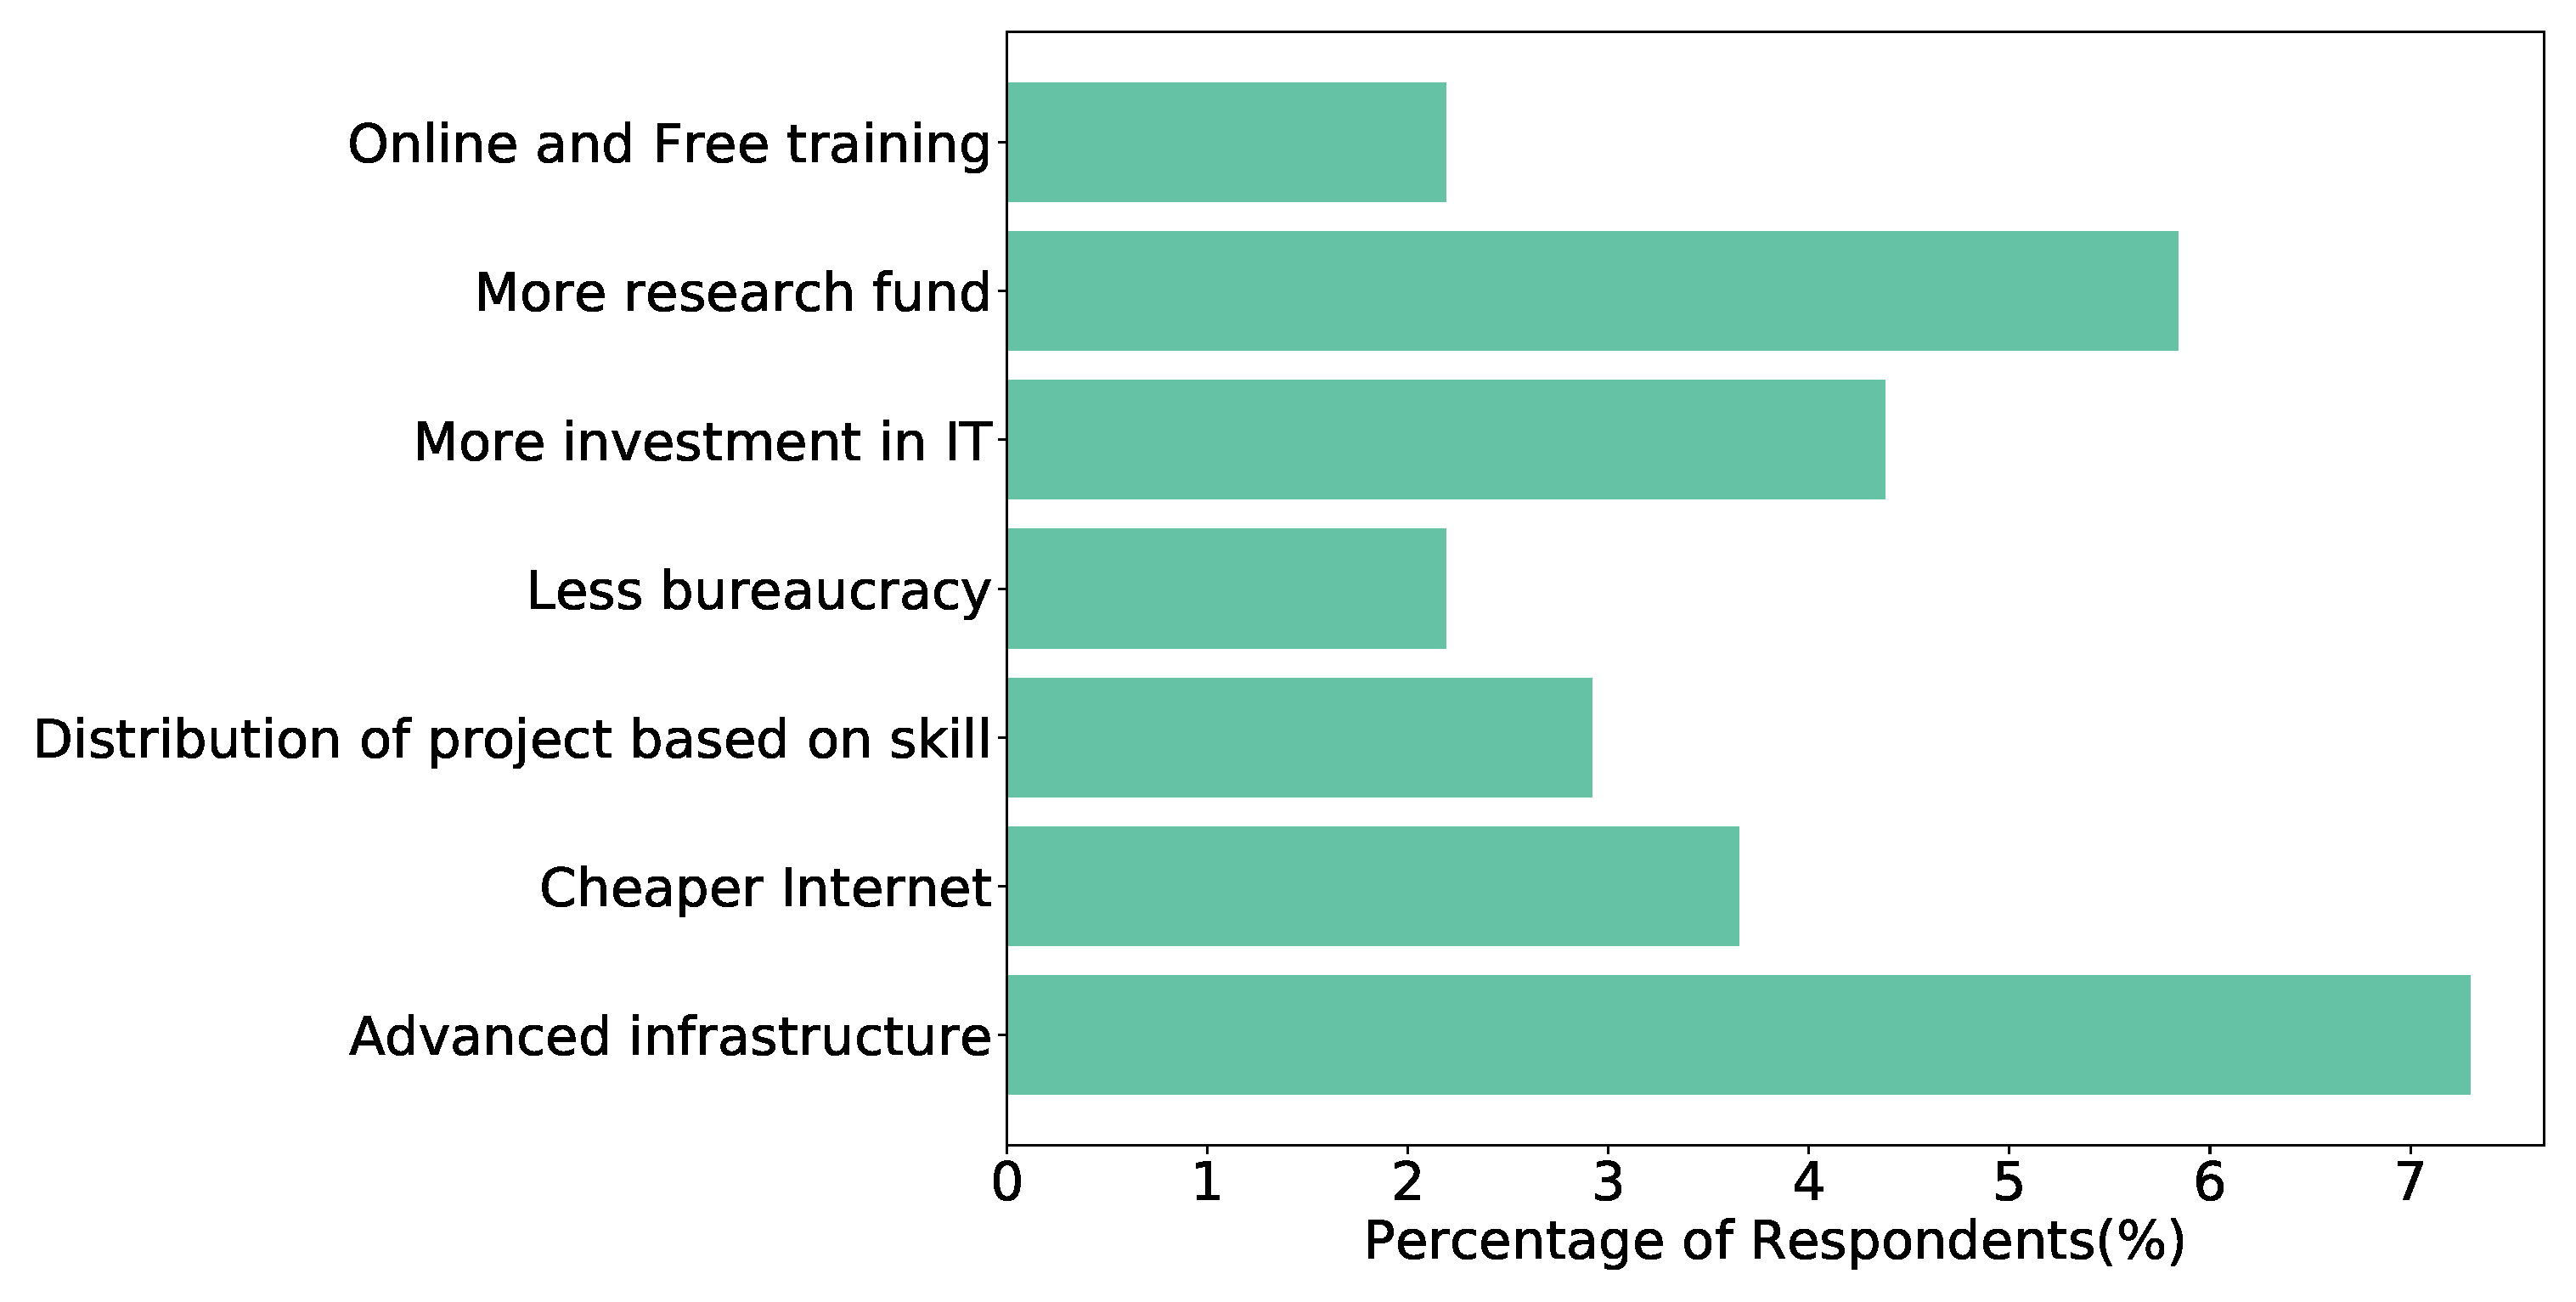
\includegraphics[scale=0.28]{Figures/GovernmentExpectation.eps} 
\caption{Respondents expectation from governmentt}
\label{fig:government expectation}
\end{figure}
\hfill\\
Government policies shapes the future SE industry. Tessler et al.\cite{Tessler2003} completed a study to rank the possible action for government for boosting the IT industry. They have ranked infrastructure and telecommunication as the first two action for government. The result is similar to our study where the 7.3\% respondents  expects  better infrastructure from government.
\begin{enumerate}
    \item \textbf{Online and free training}: If government arranges free and online training, the professionals can learn a lot more alongside with the private training. 2.19\% of our respondents have demanded for free online workshop.
    \surveyquote{1.online Free training center for easy learning it from Advance level (industry level) , Not basic level}{128}
    
    \item\textbf{More research fund}: In our country, research funds issued by government is really really less than expected. If we want to emerge as a country of developed software industry, government have to issue more money on research on this sector. 5.84\% respondents think that it is very hard to develop software industry with such little funds.
    \surveyquote{Issuing research funds to the universities to run researches. Government should emphasize in automation in every possible sector}{10}
    
    \item\textbf{More investment in IT}: 4.38\% respondents wants more investment  in IT sector from the govern met. Respondents mention steps like tax waiver and creating opportunities for domestic companies in government projects.
    \surveyquote{Tax benefits, infrastructure}{66}
    
    \item\textbf{Less bureaucracy}: 2.19\% of respondents want the removal of red tape from the administrative process as it prevents the development of the IT industry.
    \surveyquote{get yourself out of corruption. and let yourself put in liability}{133}
    
    \item\textbf{Distribution of project based on skill}: It is frequently seen in our country that less expert and less eligible persons are getting priority than more eligible persons because of nepotism. 2.92\% of our respondents think that it should be eliminated as soon as possible for the sake of industry development.
    \surveyquote{Proper maintenance with previous projects and follow up. Plan next years with long vision through solid IT-specialists. Distribute projects based on skills than links. Remove bureaucratic process for small companies to contribute more for country}{5}
    
    \item\textbf{Cheaper internet}: In this age, it is difficult to spend a single day without internet. As it is also a great source of learning as well as earning, government should remove tax from internet charge and give internet in exchange of a very lower rate. Some people have also asked for 5G.
    \surveyquote{faster and cheaper internet infrastructure}{74}
    
    \item\textbf{Advanced infrastructure}: 7.3\% respondents expects advanced infrastructure like IT/software parks, data center from government.
    \surveyquote{Improved transport system, Software development zone with competitive rent}{85}
    
\end{enumerate}

\subsubsection{Training provide by Companies}
\label{Training provide by Companies}
\begin{figure}[htbp]
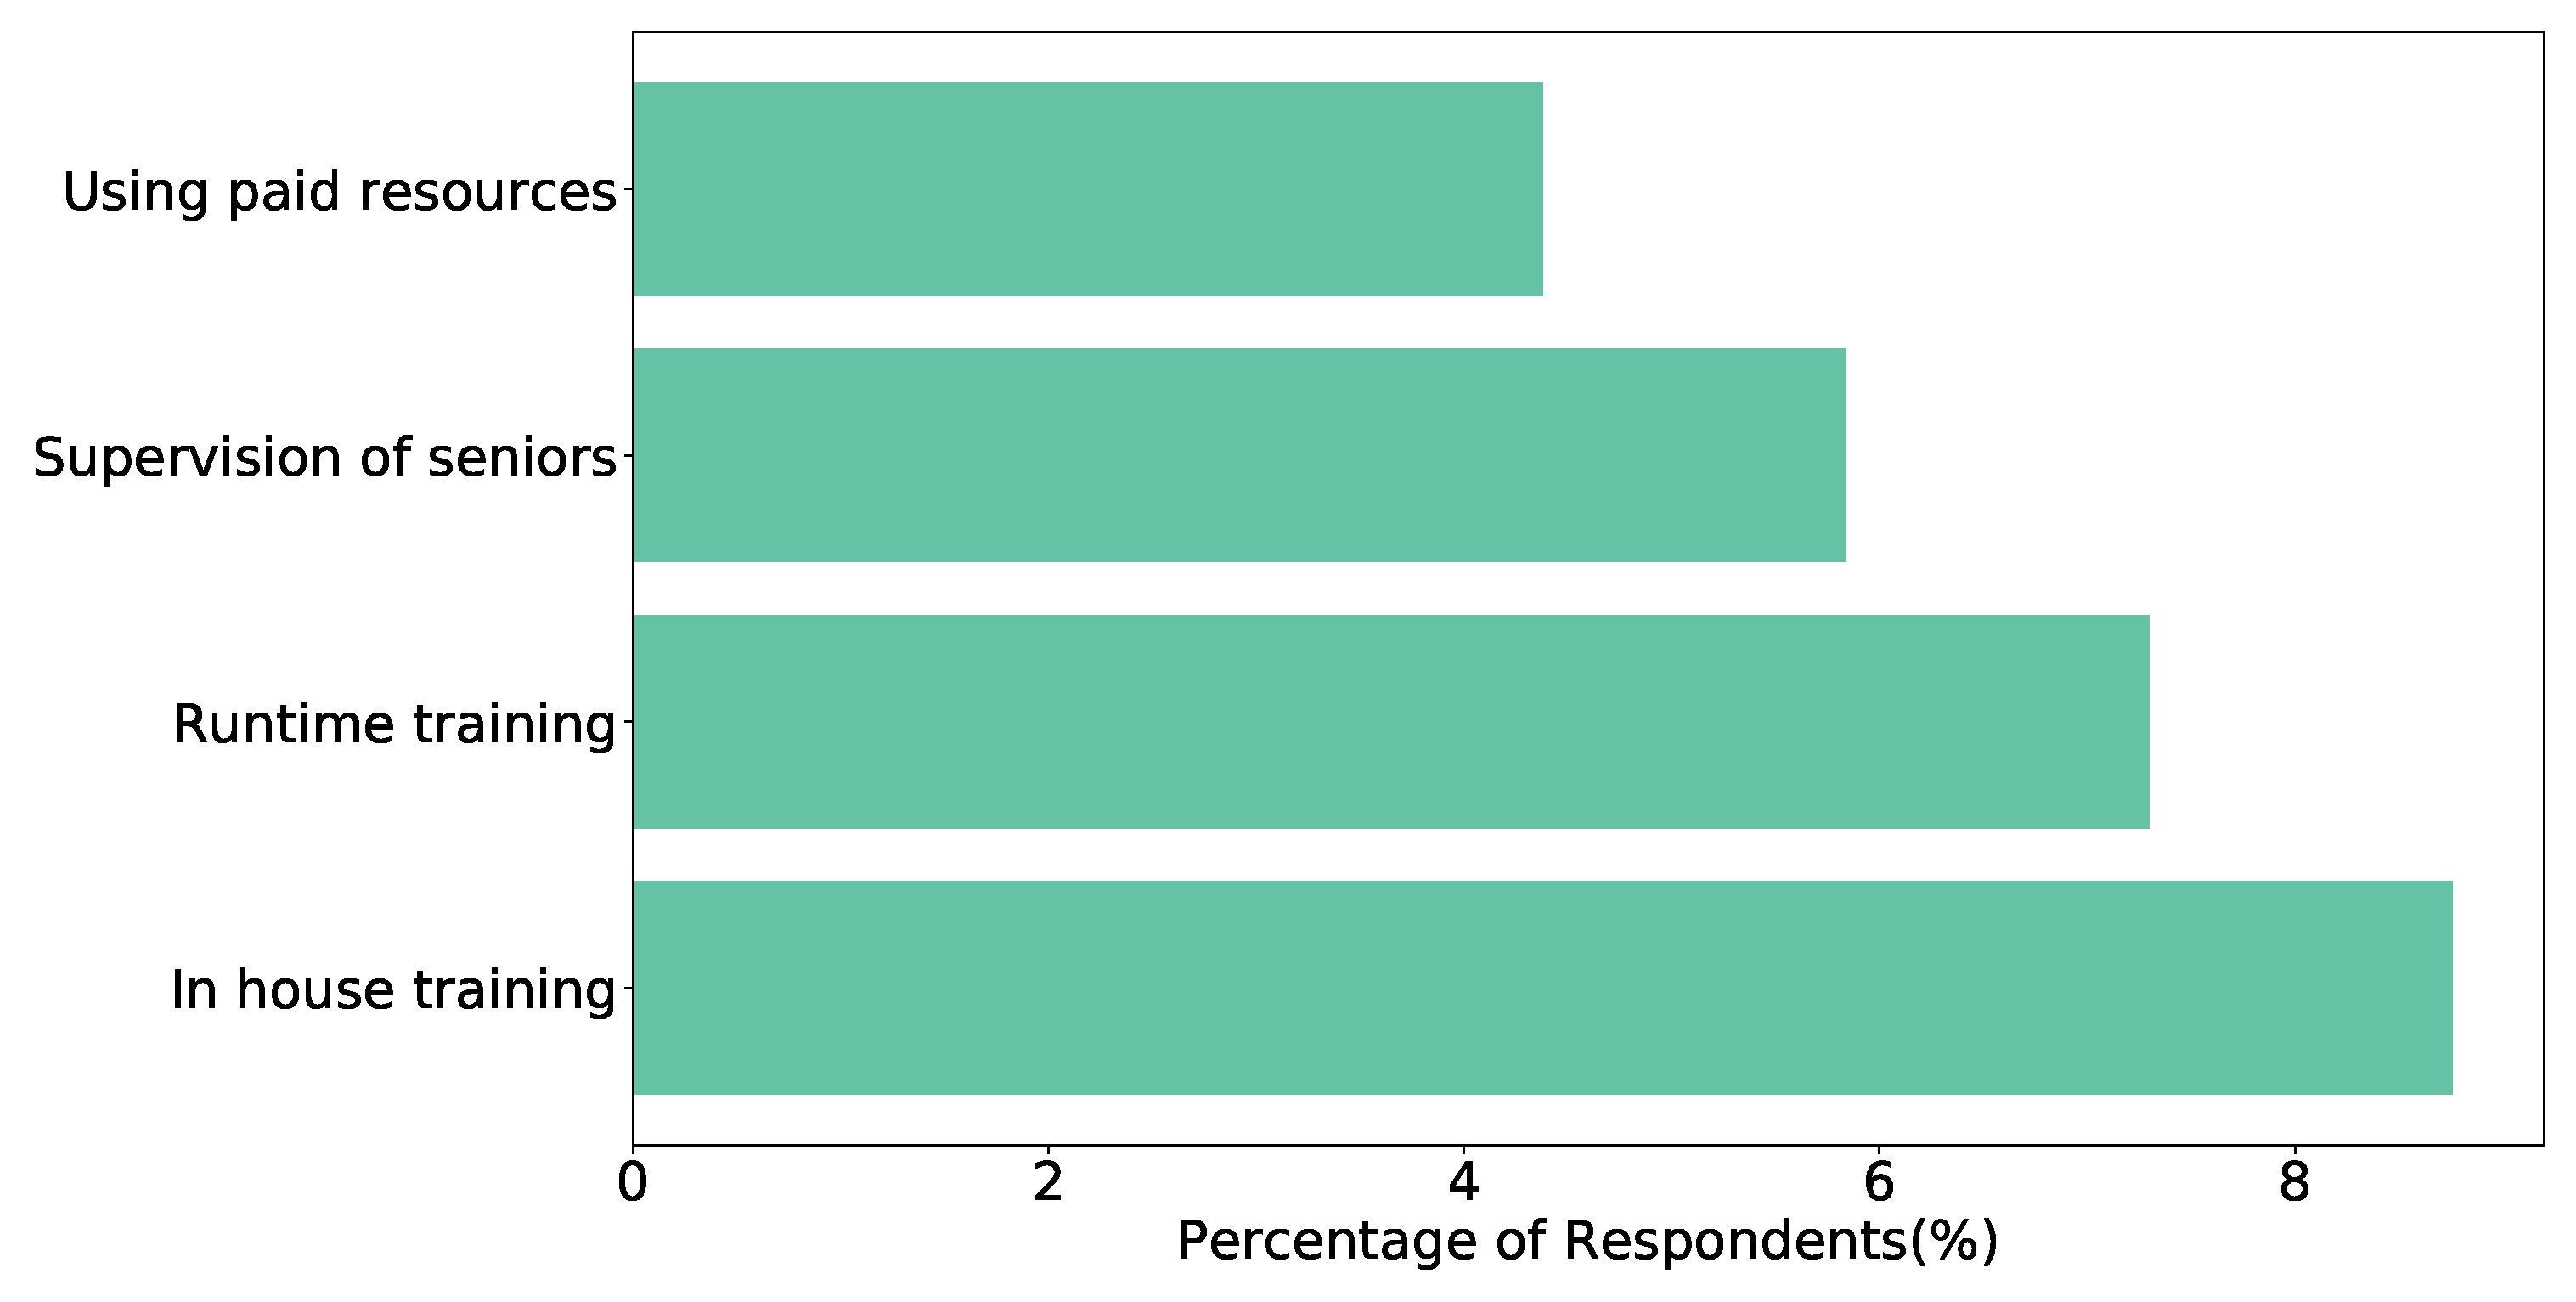
\includegraphics[scale=0.28]{Figures/Training.eps} 
\caption{Respondents expectation from government}
\label{fig:company training}
\end{figure}
\hfill\\
In order to adapt to the new technologies and drive new employees, staff training sessions are required in SE firms. From the survey, it is clear that in house training is the most popular form of training in the SE industry in Bangladesh. In the Australian \cite{Ng2004} and Hong Kong\cite{Chan2005} SE industry , the scenario is different where the most popular form of training is commercial courses and then in house training.  The difference in popularity can be linked to economic conditions. As the SE industry of Bangladesh is not mature, it is clear that SE companies will not be able to spend money on paid training courses.

\begin{enumerate}
    \item \textbf{Using paid resources}: 4.38\% respondents mentioned that they use online paid resources or certification courses to train their employees.
    \surveyquote{We have pluralsight account and we perform bimonthly technical session}{57}
    
    \item\textbf{Supervision of seniors}: Being supervised by the seniors is the best way of training. They can teach us from their experience and experience teaches a lot.
    \surveyquote{mentoring}{74}
    
    \item\textbf{Runtime training}: About 7.3\% people have said that they provide their employees with runtime training.
    \surveyquote{Run time training through small scale project and supervision of seniors}{5}
    
    \item\textbf{In house training}: Companies also provide their employees with tutorials and books so that they can read at their home and get used to the practices followed.
    \surveyquote{Internal knowledge sharing sessions}{53}
    
\end{enumerate}



% \input{Sections/Implication}
% \section{Threats to Validity}
\label{validity}

\subsection{Construct Validity}
% Construct validity threats concern the relation between theory and
% observations. 
Construct validity is mainly concerned with the extent to which the
study objectives truly represent the theory behind the study\cite{Wohlin2012}. In our study, we have used open coding strategy to label the survey responses. The nature of this coding strategy may introduce researcher bias into coded labels. To mitigate the issue, the labels have been coded by two individuals, and the codes are accepted when there is a reasonable agreement among the coders. Another issue can be whether our data actually represents real-world SE practices. This study counted the votes and made statistical inference, which is common in survey-based studies. It is believed that voting data can, to a certain extent, reflect the opinions of the majority. It was previously observed\cite{Garousi2015} \anindya {where observed? cite?}\partha{added} that people tend to form their answers close to expected answers when evaluated. To mitigate the threat, before the survey, we informed participants that our motive in this survey was to get a decent understanding of current practices, and we do not intend to collect any personally identifiable data. Construct threats may also be introduced by a misleading interpretation of the survey questions. We conducted a preliminary survey and interview session with some participants to rule out any ambiguity from survey questions and thus tried to reduce such risk.

\subsection{Internal Validity}
% Threats to internal validity refer to how well the research is
% conducted.
Internal validity is a property of scientific studies that refers to how well a study has been conducted. A threat to internal validity in this study is inherent in the participant selection bias. We used several social platforms, personal connections to reach as many participants as possible. Another threat could arise from the placement of the options in a multiple-choice question. It is often observed that survey participants often show bias towards the first option in any multiple-choice question\cite{Uddin2019} \anindya{Can you cite?}\partha{added}. However, in one of the multiple-choice questions (Q9), the `Web' option was placed at the bottom of the list. Despite this placement, we observed most of the participants selected `Web' as a technology platform. But practically, from the personal experience of the authors, there is no bias in this opinion.


\subsection{External Validity}
% Threats to external validity compromise the confidence in stating
% whether the study results apply to other groups.
External validity is concerned with the generalization of the study result. In our study, we have participants from almost all the groups of the Bangladesh software industry. However, it is difficult to claim the statistical generalizability of our findings, given that our sample included 137 respondents where there 1100+ companies and 3,00,000 IT professionals\cite{BASIS2018} in the software industry of Bangladesh \anindya{make it consistent with intro.}\partha{updated}. Moreover, emerging IT industries share a common trend of challenges\cite{Sison2006, lloyd2020}. Thus, our findings are also applicable to other emerging software industries across the globe.
% \section{Conclusion}
\label{sec:conclusion}
Thanks to the results of this survey, we have observed that software industry in Bangladesh is
spirited, growing and competitive that many software teams are eager for adopting state-of-theart software engineering practices and approaches.Awareness and knowledge about these practices and approaches are rising in the industry, that many organizations have been establishing
them within their development operations. We have also observed that the industry needs to
improve on using well-established requirements engineering and testing related practices.These
two areas are where most displeasure is stated about. Also we observed that practitioners have
a tendency to avoid formal or relatively complex best practices (e.g.TDD, formal languages,
pair programming, automation testing and metric usage) in general, but especially in these two
areas. We suggest organizations to invest in improvement and training efforts for increasing
the awareness and knowledge about these software disciplines.In this study, we have seen that
social aspects are important as well that many practitioners have expressed their discontent and
difficulties on issues like communication, collaboration, and team structure.


\bibliographystyle{ACM-Reference-Format}

\bibliography{bibliography}

\pagebreak
\appendix

    
\end{document}